\documentclass{book}
\usepackage{graphicx} % Required for inserting images
\usepackage{svg}
\usepackage{pifont}
\usepackage[T1]{fontenc}
\usepackage[final]{microtype}
\usepackage[hidelinks]{hyperref}
\usepackage{tabularx}
\emergencystretch=1em

% Fancy enumerations for our letter-number references like requirements, protection goals and more
% From: https://tex.stackexchange.com/questions/1230/reference-name-of-description-list-item-in-latex
\usepackage{enumitem, hyperref}
\makeatletter
\def\namedlabel#1#2{\begingroup
    #2%
    \def\@currentlabel{#2}%
    \phantomsection\label{#1}\endgroup
}
\makeatother

% Listings (unknown source)
\usepackage{listings}
\definecolor{codegreen}{rgb}{0,0.6,0}
\definecolor{codegray}{rgb}{0.5,0.5,0.5}
\definecolor{codepurple}{rgb}{0.58,0,0.82}
\definecolor{backcolour}{rgb}{0.95,0.95,0.92}

\lstdefinestyle{codestyle}{
	backgroundcolor=\color{backcolour},
	commentstyle=\color{codegreen},
	keywordstyle=\color{magenta},
	numberstyle=\tiny\color{codegray},
	stringstyle=\color{codepurple},
	basicstyle=\ttfamily\footnotesize,
	breakatwhitespace=false,
	breaklines=true,
	captionpos=b,
	keepspaces=true,
	numbers=left,
	numbersep=5pt,
	showspaces=false,
	showstringspaces=false,
	showtabs=false,
	tabsize=2,
    xleftmargin=2em,
    framexleftmargin=1.5em
}

\lstset{style=codestyle}

% Longtable
\usepackage{longtable}

% -- for comments
\usepackage{xcolor}
\usepackage{soul}
\newcommand{\cgn}[1]{\textcolor{brown}{[GN]: #1}}
\newcommand{\cts}[1]{\textcolor{red}{[TS]: #1}}
\newcommand{\cfw}[1]{\textcolor{blue}{[FW]: #1}}

\usepackage[defernumbers=true]{biblatex}
\addbibresource{bibliographies/1_introduction.bib}
\addbibresource{bibliographies/2_background.bib}
\addbibresource{bibliographies/3_related_work.bib}
\addbibresource{bibliographies/4_methodology.bib}
% \addbibresource{bibliographies/5_design.bib}
\addbibresource{bibliographies/6_implementation.bib}

\title{Thesis}
\author{Fritz Windisch}
\date{September 2023}

\begin{document}

\maketitle
\chapter*{\centering Abstract}
In the current world of IoT a lot of small devices flood our networks that are prone to vulnerabilities due to infrequent updates and critical vulnerabilities shipped from factory. Due to this, network engineers are challenged with a new level of threats on their networks, calling for a zero trust approach of all participating devices. Network slicing is an integral part of protection against these threats, as it provides the necessary isolation required for a zero trust approach. There is however currently a lack of network slicing solutions that span multiple domains and have investigated security aspects thoroughly enough for deployment in mission critical contexts. In this thesis we thus wish to build a network slicing architecture spanning multiple domains with a focus on security and resilience.
% Content source: https://tu-dresden.de/ing/elektrotechnik/iee/hpsn/ressourcen/dateien/Statement_of_Authorship.pdf?lang=en

% TODO: Swap with computer science text

\chapter*{Statement of Authorship}

I hereby declare that I have written this thesis independently and have listed all used
sources and aids. I am submitting this thesis for the first time as part of an examination. I
understand that attempted deceit will result in the failing grade „not sufficient“ (5.0).\\[4ex]

\renewcommand{\arraystretch}{0}
\begin{table}[h]
    \begin{tabularx}{\textwidth}{ llX }
        Dresden, on the 09/13/2023 & \hspace{40pt} & \hrule                                             \\
        &               & \begin{flushright}
                              Fritz Windisch
        \end{flushright} \\
    \end{tabularx}
\end{table}
\renewcommand{\arraystretch}{1}

\tableofcontents

\chapter{Introduction}
\begin{itemize}
    \item Motivation $\rightarrow$ With threats
    \begin{itemize}
        \item Focus on the current IoT domain and the existence of critical communication channels
        \item Provide example of remote surgery
        \item State some threats to this communication channel (CIA) - those will be picked up and formalized in the related work chapter
    \end{itemize}

    \item Objective
    \begin{itemize}
        \item
    \end{itemize}

    \item Structure
\end{itemize}

\chapter{Background}
\label{background}

Considering our remote surgery example and the threats we face, we now want to establish protections against these threats. To provide accurate protections we first have to analyze our domain. To do this, we will talk a bit about network security and edge computing in general. We will then focus on common concepts that can help us secure our communication, investigating quality of service (\acrshort{qos}) and network slicing. After this we will have a closer look on technologies that can help us along the way to realize the aforementioned concepts.
%In this chapter we will establish some common terms concerning the technical background of this thesis. First we will describe our domain of network security and edge computing, before introducing key technologies that have been used such as software defined networks (\acrshort{sdn}), network function virtualization (\acrshort{nfv}), service function chaining (SFC), virtual private networks (\acrshort{vpn}) and multi protocol label switching (\acrshort{mpls}). Lastly we will focus on concepts like quality of service (\acrshort{qos}) and network slicing.

%\cgn{The current content of the background already contain good building blocks. However, it is hard to see the coherent connections between the blocks. I suggest a different order of writing: \begin{enumerate}
%    \item Use case: Human-Machine (or robot) interaction -- HCI (?) -- because networks are built for a purpose. And the purpose here is real-time communication between humans and robots, requiring multiple modalities (video, video, control, haptics, etc.). Multiple modalities with different requirements on \gls{bandwidth}s, delay, jitter, etc. raise the need for \acrshort{qos} and slicing.
%    \item Network domains and edge computing: to enable low-\gls{latency} communication with direct edge-to-edge connections via autonomous systems. This sections, therefore, includes enabling technologies, such as \acrshort{nfv}/\acrshort{sdn}
%    \item \acrshort{mpls} (for tunneling / routing between AS) and \acrshort{vpn}
%    \item Service differentiation (\acrshort{qos}, slicing)
%    \item (Network) Security, especially for mission critical use cases. At this point, it is natural to discuss the (security) requirements for the systems or networks you will discuss in Related work.
%\end{enumerate}
%By the way, I am unsure about the role of \acrshort{2pcp} and SFC in this thesis. However, it is possible that I didn't read it through. Therefore, as long as you can find a logical order for them, it should be good.
%}
%\cfw{I tried to spin the order by the three categories I used, structuring the content by the similarity of role in this thesis. Maybe the story reference could be placed in the beginning of the background and I could introduce the story as motivation in the introduction. I guess I could still spin the story in a way that it makes sense to begin with network security though, because consequences of failure could have been averted by designing the network with security in mind, introducing our domain. Then we can go to edge-computing to understand in which domain we are working. ("But to understand how we can secure our communications in the future, we must first understand or domain...") Then I could move up the concepts to say "this is how we could have had more security" and then state the building blocks (enabling technologies) that will help us build a better solution. This way I could connect all the blocks with a story by stating their relevance in the beginning and providing some links. Does that sound like a good idea? :) }


\section{Domain}
Considering our domain we locate ourselves in the network security context. We will thus first shed some light on this topic, because without knowing what security is we can not claim that something is secure. Afterwards we will focus on our general network architecture that we wish to secure communications on, which is edge computing.

\subsection{Network Security}
In order to secure communications in a network, we have to first define what network security is. According to \cite{netsec}, network security can be viewed as a subset of computer security, focusing on network-perimeter and computer system security. Some means to achieve this include, but are not limited to, computer intrusion detection, traffic analysis and network monitoring. Computer intrusion detection can be realized by installing intrusion detection software on systems that should be protected or by deploying honeypots \cite{honeypot}. Honeypots are systems that are supposed to be targeted by attackers in order to detect and distract them. By using honeypots one can learn what the attacker is going to try and ideally deploy protective measures before the attacker reaches a real system that needs to be protected. Traffic analysis on the other hand can be used to detect attacks based on traffic shapes that are unusual compared to normal operation. The same applies to network monitoring which instead focuses on events in the network.

Another view on network security can be from the cryptographical standpoint \cite{netsec}. Cryptography plays a key role in network security, because it can be used to achieve four of the major goals of security in network contexts: confidentiality, integrity, authentication and non-repudiation \cite{cryptography}. In this context security-games are often played to define what an attacker may know or does not know at a certain point of a secure protocol, e.g. a key exchange, and what the attacker can possibly guess \cite{games}. The assumption generally is, that while some parties are honest and behaving according to protocol, some malicious actors will participate in the protocol. These malicious actors should (hopefully) never reach their goal concerning the protection goals from above.

So while the two views presented so far are of different nature, what combines them is the set of major protection goals on a network. Here are some of the most noteworthy \cite{goals}:

\paragraph{Confidentiality} Information that is only meant to be viewed by certain parties must not be disclosed to other parties.

\paragraph{Integrity} Unauthorized modification or forgery of information has to be detected.

%Information has to be protected against modification or forgery by malicious actors. \cts{I think protecting it is difficult, but we have to provide functionality to detect if transmitted data has been tampered with, or forged.}

\paragraph{Availability} Provided services should be reachable and functional at all times without interruption.

%Information has to be available according to the service specifications. \cts{Authorized parties should be able to use services at all specified times without interruption.}

\paragraph{Controlled access} Actors must not be able to perform actions on objects they are not permitted to.

\paragraph{Non-repudiation} Actors must not be able to claim that they did not take part in an action.

%\cts{one could argue that authentication is less of a goal than a service, but controlled access would be a goal (note the Schaefer/Rossberg book, which picks the five of CIA + controlled access + non-rep ;)}
%\cfw{I did some research on the book and adapted the protection goals accordingly, while swapping out the source :)}
%\cts{looks good}

\paragraph{} Apart from this there also exist other security services, such as \textit{authentication} (The claimed identity of all entities can be verified) and \textit{authorization} (Entities have a set of permissions that can be managed by privileged entities and are encoded in a policy), which are required to implement confidentiality, integrity, controlled access and non-repudiation.

%\cts{well I'm not sure if they're requirements as such, but they are required to be able to implement integrity, controlled access and confidentiality (can't check if the source of a message is legit if you can't verify the identity of the source...}

%\cfw{Are these descriptions accurate?}

\subsubsection{Resilience}
Furthermore, resilience of networks can be an important goal \cite{resilience}. According to Trivedi et al. \cite{resilience}, resilience of a network or computer system is the combination of trustworthiness and tolerance.

\paragraph{Trustworthiness} consists of:
\begin{itemize}
    \item Dependability (How reliable is the system?)
    \item Security (Which risks does a system have?)
    \item Performability (How capable is a system?)
\end{itemize}

\paragraph{Tolerance} consists of:
\begin{itemize}
    \item Survivability (How likely will a system survive when target of an attack?)
    \item Disruption tolerance (How well does the system handle service disruptions?)
    \item Traffic tolerance (How much traffic can the system handle?)
\end{itemize}

\paragraph{}When one of the six components of resilience is impeded, the major protection goals might be compromised. This is why resilience should play a key role when designing networks and services.

\paragraph{}So as one can see, network security is a relatively complex topic with many different approaches, view angles and goals. But while different approaches exist, it is of critical importance today to design networks with security in mind. Network outages can cause a lot of damage to property or infrastructure, prompting for security-aware solutions in the current world of digitalization. In our example of a surgery, the outcome could even be worse than just monetary damage.
%\cts{sounds good. You have a weird way of using paragraphs, why not simply end the paragraph with an empty line, or if you need more space end the last line of the previous paragraph with a double back-slash?}

\subsection{Edge Computing}
In our use case, we wish to communicate between two networks that are connected via multiple other networks. This means that opposed to the centralized approach of communicating from a remote client to a centralized server, we are communicating from one remote client to another remote client. This offloads computation from central servers to the edges of the networks.

Edge computing \cite{edgecomputing} refers to this relatively new approach, performing computations at the network edges, closer to the end user. As previously mentioned, the internet of today still follows a mostly centralized approach with servers clustered in data centers while users remain at the edges of the network.

This provides some challenges to the network though, because the traffic has to be transported over long distances. This has significant impact on \gls{latency}, \gls{bandwidth} at central hubs, security and privacy. By moving the computational resources (e.g. servers) closer to the user at the network edge, we can reply to requests from the user with less delay, with less transportation distance (and thus cost) and with more security and privacy in mind due to decentralization.

This also reduces the possible single points of failure because there is no central infrastructure anymore that could render a service unusable for all users. Edge computing has gained additional traction in recent developments due to the emergence of \acrshort{iot} in our everyday lifes. With a lot of data being collected by \acrshort{iot} devices, edge computing can be used to bundle all traffic generated by a users \acrshort{iot} devices closer to their origin, reducing the overall load of networks and thus their operational cost.


\section{Concepts}
\label{bg_concepts}
Next, we will focus on the central concepts that we can use to secure our communications in the edge computing context. For this, we need to know what a good and stable communications channel is compared to a bad one. Therefore we will introduce quality of service (\acrshort{qos}) and different metrics associated with it. Afterwards we are going to establish network slicing as a concept to help us guarantee meeting certain \acrshort{qos} parameters for our communications, which will help us eliminate our threats later.

\subsection{Quality of Service (QoS)}
% TODO: Maybe find a better base source for this chapter? --> It is hard to find a good source for such an old and basic term, thus the IP has been included for intial references of \gls{latency} (delay), throughput and \gls{lossrate} (high-reliability). The main qos source mentions the 4 terms below (as many other papers do).
For now, we just talked about securing our communications to always have an usable connection. But so far we have not talked about how a connection can be guaranteed to remain usable at all times. For this, the concept of quality of service (\acrshort{qos}) has been created.

Quality of service \cite{qos, rfc791} refers to assigning traffic to flows for which certain guarantees are to be upheld. These guarantees are usually measured in different metrics, of which the major four are outlined here:

\paragraph{Latency} The two-way delay for a packet travelling from flow start to finish and back.

\paragraph{Jitter} The mean deviation of \gls{latency} from the mean \gls{latency} (standard deviation).

\paragraph{Throughput} The number of bits transferable in one direction via the traffic flow in a certain time.

\paragraph{Loss rate} The number of lost packets divided by the total amount of packets. The \gls{lossrate} is especially relevant in contexts where data needs to be transmitted again when lost, because the lost data will then need to be requested again and will be delivered delayed, thus at least doubling the \gls{latency}.

\paragraph{}Securing these guarantees is an important task in network security, as violation of them could result in service level agreements (\acrshort{sla}s) being broken and violation of availability as one of our main goals.

To determine the flow for a certain packet, two main approaches exist \cite{serv}:

\paragraph{\acrshort{intserv}} Integrated Services \cite{rfc1633} negotiate flows beforehand with all participating network nodes. Packets are then assigned to flows based on pre-negotiated parameters. The advantage of this approach is that \gls{bandwidth} and other assigned guarantees can be planned by the participating network providers in advance.

\paragraph{\acrshort{diffserv}} Differentiated Services \cite{rfc2474} on the other hand match quality of service on a per packet basis, normally by using the \acrshort{ipv4}/\acrshort{ipv6} differentiated services (DS) header field. The advantage of this approach is that it provides flexibility to the sender of packets who can assign priorities per packet. The disadvantage is of course that network operators can not plan ahead accurately before packets arrive and providing guarantees will be challenging.

\subsection{Network Slicing}
Now that we know what we can guarantee to a communication flow, we still have to technically be able to realize these guarantees. This is where the concept of network slicing comes into play.

Network Slicing \cite{slicing} refers to partitioning part of the resources of a network to new virtual networks. Partitioned resources can include network resources, computational resources and storage resources. The result are multiple virtual networks that each have a slice of the resources of the underlying network available and guaranteed to them. In order to guarantee these resources to the owners of a slice, the slices need to be isolated from a resource perspective.

The latest developments in the field are part of the 5G standard, where applications can request slices of network resources to leverage uninterrupted communication afterwards. Apart from 5G also other applications leverage this approach already, for example by partitioning network links on nodes with multiple virtual machines.


\section{Enabling technologies}
In our concepts (section \ref{bg_concepts}) we stated that we want to isolate communication flows by performing network slicing. But in order to create network slices, we need technologies supporting us at this task. We will first focus on how we can orchestrate such a dynamic network, focusing on software defined networking (\acrshort{sdn}), network function virtualization (\acrshort{nfv}) and synchronization paradigms such as the two-phase commit protocol (\acrshort{2pcp}). Afterwards we will discuss some means to provide private and resource isolated communications through multiple networks in the form of virtual private networks (\acrshort{vpn}).

\subsection{Software Defined Networking (SDN)}
When building network topologies, software defined networking \cite{sdn} has emerged as one of the most valuable tools to build networks dynamically and with lower cost.
While traditionally specialized hardware was deployed for every use case, \acrshort{sdn} provides a number of abstractions to build arbitrary virtual topologies on top of real-world topologies.
To achieve this, software defined networking partitions the network into three major planes:
%\cts{is the notion of 'higher' and 'lower' layers useful in the context of \acrshort{sdn} (Giang?)? For me when it comes to networking higher layers are those closer to the application and lower layers those closer to the medium (iso/osi, tcp/ip models). Not sure..}
%\cfw{Ah, most likely not. But I can simply omit "lowest" like I now did below :)}
%\cgn{\acrshort{sdn} usually uses plane instead of layer}
%\cfw{I changed "layer" to "part of the infrastructure" below - hopefully now everything is correct :)}

\begin{figure}[h]
    \centering
    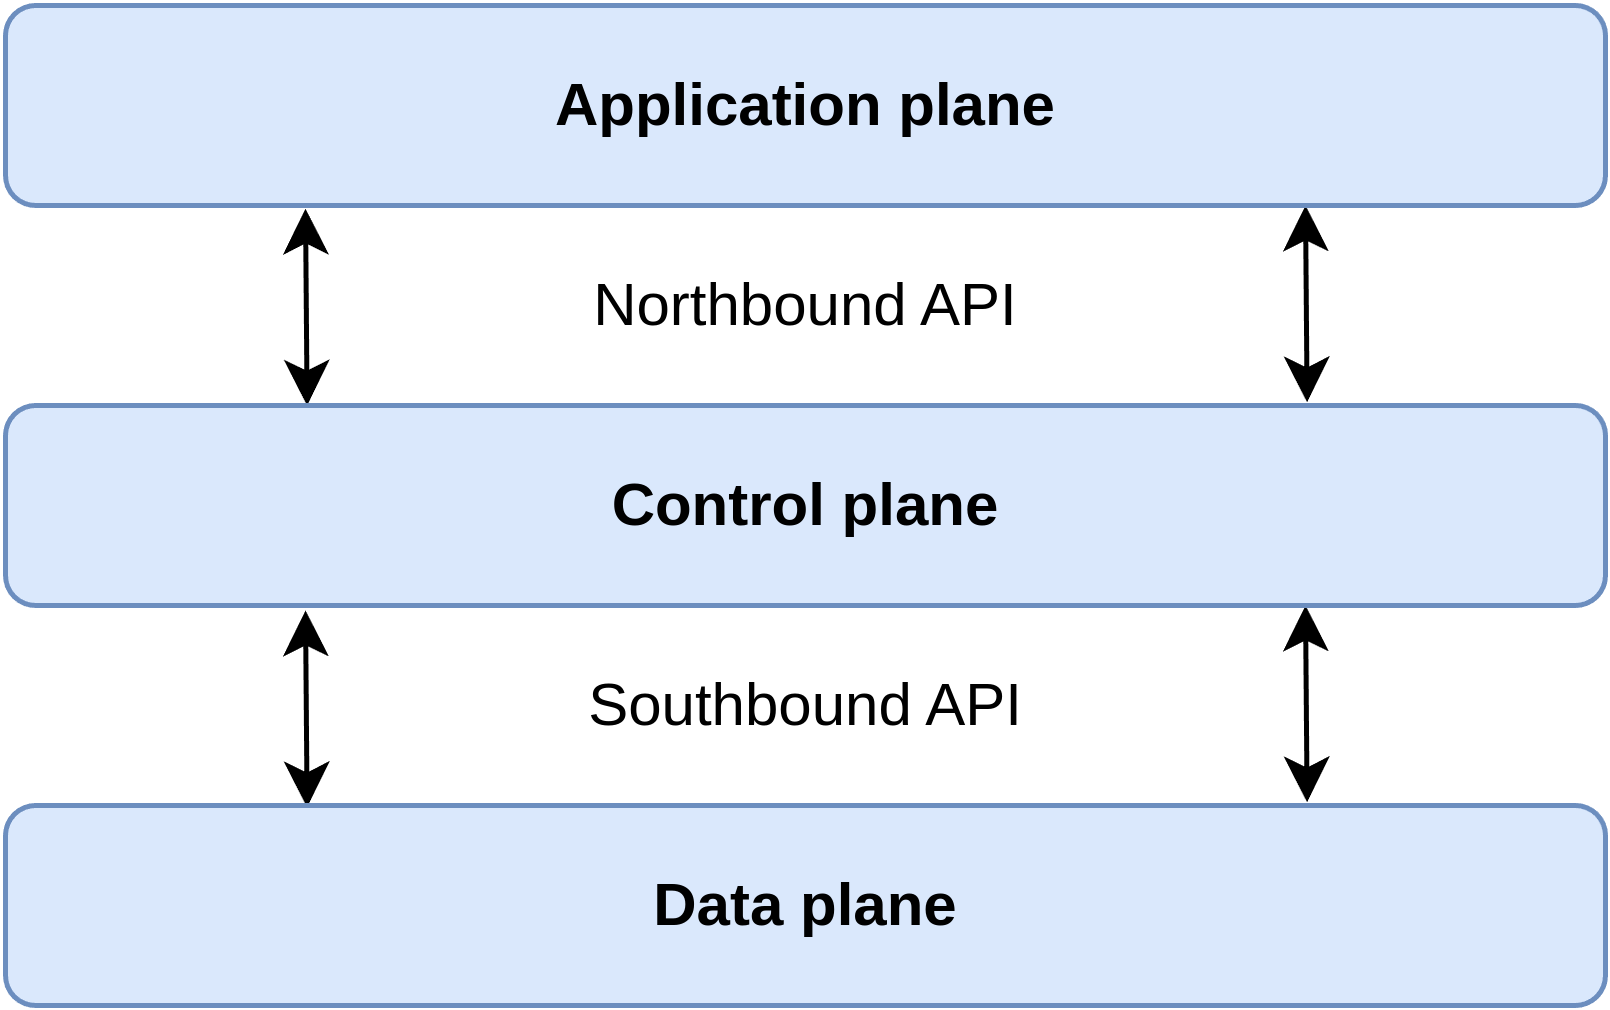
\includegraphics[width=5cm]{images/chapter_2/sdn.png}
    \caption[Software defined networking (\acrshort{sdn})]{The three planes of software defined networks: application plane, control plane and data plane. Application and control plane are connected via northbound \acrshort{api}s, while control and data plane are connected via southbound \acrshort{api}s like \Gls{openflow}.}
    \label{fig:sdn}
\end{figure}
%\cts{the figures are *very* large. As a rule of thumb, the text in a figure should never be as large as the text of the surrounding environment (rather smaller)}

\paragraph{Data plane} This is the part of the infrastructure actually performing the work on the data to be transmitted. It is usually being realized by switches or other hardware that is used to perform work on the network traffic itself.

\paragraph{Control plane} The control plane consists of \acrshort{sdn} controllers that instruct the data plane components on how to handle data via a southbound \acrshort{api}. The data plane components will also contact the control plane when instructions for a certain type of traffic are needed that no rules have been defined for yet.

A commonly used protocol and the defacto standard for this southbound \acrshort{api} is called \Gls{openflow} \cite{openflow} and is currently supported by a wide range of \acrshort{sdn} capable switches. With OpenFlow, traffic is being classified into flows via flow matching tables. After traffic has been assigned to a flow, the actions that have been defined for this flow will be applied on the traffic by the data plane components. Actions include dropping traffic, queuing traffic, outputting traffic on a specific port and modifying traffic in various ways.

\paragraph{Application plane} This plane is used to configure the \acrshort{sdn} controllers via a northbound \acrshort{api}. This can include end applications and users that want to manage and monitor the network.

\paragraph{}These three planes can also be seen in figure \ref{fig:sdn}.

\subsection{Network Function Virtualization (NFV)}
Closely related to \acrshort{sdn} is the concept of network function virtualization \cite{nfv}. Network functions are components taking a specific role in a network, such as a switch which would forward or reshape traffic. Originally a lot of proprietary network functions were used to create larger networks. This resulted in a difficulty to manage the resulting networks. The proposed solution proposed for this is virtualization, so that individual network functions are decoupled from their hardware and executed in a virtual environment. The resulting network functions are called virtual network functions (\acrshort{vnf}s) and can be orchestrated with ease to build complex topologies and integrations on a network level. Virtual network functions can thus be used as building blocks for software defined networks.

%\subsection{Service Function Chaining (SFC)}
%In order to interconnect our virtual network functions mentioned previously, service function chaining \cite{sfc} has emerged to connect different network functions to each other. According to Bhamare et al. \cite{sfc}, it is thus a key enabler for network function virtualization. The problem without service function chaining is, that network functions need to be linked to each other statically by providers. This provides significant effort to the network administrator to configure each connection manually in a static environment. With service function chaining, a virtualized software defined infrastructure is created connecting one network function to another, effectively forming a chain of service functions. To achieve the connections, a service function chaining architecture is used, of which multiple approaches and implementations currently exist. A common approach suggested by RFC 7665 \cite{rfc7665} is to encapsulate packets with an additional header (or additional information) that specifies the service function that the traffic should be steered towards. This header can either be added by a service function that is aware of the chain, or if the service function is not chain-aware it can be added after leaving the service function by the next network device the packet traverses to achieve easier routing of traffic. The standard also warns though (in section 5.6), that this could lead to a decrease in the maximum transmission unit (MTU), the maximum size the content of a packet may have on the network.

%\cts{two things: (1) are we using service function chaining later? I wouldn't introduce it otherwise.
%(2) mini English writing primer: text is structured in sentences, paragraphs, subsections, sections, and chapters. Each sentence should contain exactly one (and no more) statement. Each paragraph should group the statements that explain/discuss one (and no more) atomic concept/thought/idea. (Sub)sections group the paragraphs that discuss/explain one complex concept/thought. The abstraction layer throughout all paragraphs of one section should be identical (abstract vs technical vs detailed vs formal-with-variables/equations).
%The paragraph in 2.2.3 is too complex as it discusses different aspects of SFC. If we keep it, it should be cut to several paragraphs. ((2) is relevant for the entire thesis, of course ;-p)}

%\cfw{I will split the topic up, if we keep it. We currently use parallel structures to SFC in our thesis, so it is really only mentioned in one sentence in the design. All the \acrshort{vnf}s from the application are usually adressed directly without SFC. But on the data layer, the \acrshort{mpls} tag with slice id and tunnel id can be viewed as service function chaning, as the slice id specifies which starting \acrshort{vpn} gateway and which host the packet should be routed towards, while the tunnel id specifies which ending \acrshort{vpn} gateway a packet should be routed towards. So in a sense we are building a service function chain with every slice, but maybe this can already be encompassed by the \acrshort{mpls} label paragraph and we can remove SFCs all together. I just wanted to mention them for reference, but am also not an expert on this topic. So in this sense, do you think it makes sense to keep it here or should I remove it all together?}

\subsection{Two-phase commit protocol (2PCP)}
Now that we know how we can orchestrate our network components by using software defined networking (\acrshort{sdn}) and virtual network functions (\acrshort{nfv}s), we can focus on synchronization between our networks. In our example of a remote surgery we need to have multiple networks working together in order to secure our communications. We will thus need to find a way to synchronize a network slice across all participating networks. For this, the two-phase commit protocol (\acrshort{2pcp}) can be used.

The two-phase commit protocol \cite{2pcp} is a protocol used to synchronize state across transactions between multiple different participants.

The participant initiating a transaction is called the coordinator. The coordinator will send a change request to all participants of a transaction, which will take note of the changes and confirm whether their application is possible. This is also referred to as the voting phase.

Now the coordinator will proceed to the completion phase and can observe two different outcomes. The first possibility is that every participant responded that the change is possible. If so, the coordinator will send a commit message to all participants that will then apply the changes. This concludes the transaction. When the coordinator receives one failure or no reply from one of the participants though, the coordinator will abort the transaction and send rollback messages to all participants. All participants will then discard the changes, failing the transaction.

The two-phase commit protocol can not recover from a failure of the coordinator during the entire transaction or a participant during the commit phase, making it possible that an invalid state is left after a failure. We will talk about how we can secure this later in the thesis.

\subsection{Virtual Private Networks (VPN)}
In order to isolate our communications and guarantee our network resources, we will use virtual private networks (\acrshort{vpn}s).

A virtual private network \cite{vpn} is a virtual network overlayed on top of a real-world network providing private communication channels between their participants. With a lot of \acrshort{vpn} approaches and implementations in existence, they can still be distinguished by classifying them per network layer. For example there are optical \acrshort{vpn} on the physical network layer, tunnels like multi protocol label switching (\acrshort{mpls}, see section \ref{mpls}) on the ethernet layer and tunnels like \gls{wireguard} \cite{wireguard} on the IP layer. While some only participate in routing (e.g. \acrshort{mpls}), others may also encrypt traffic (e.g. \gls{wireguard}). Which \acrshort{vpn} is the correct choice thus heavily depends on the use case.

\paragraph{Wireguard} One of the most prominent \acrshort{vpn} solutions used today is \gls{wireguard} \cite{wireguard}. \Gls{wireguard} builds a tunnel between multiple participants which then form a new virtual network. The participants can then communicate via the encrypted channels established by \gls{wireguard}, which can thus traverse untrusted terrain without the fear of someone obtaining confidential information \cite{wireguard}.

Furthermore \gls{wireguard} also provides protections against attacks on integrity of data according to their whitepaper \cite{wireguard}. An attacker may not produce ciphertext themselves, because traffic is encrypted and guessing valid ciphertext that will successfully decrypt "has a negligible probability" \cite{wireguardcrypto}. To achieve protection against replaying of packets, they use nonces that are never reused but accepted in a historical window of about 2000 entries \cite{wireguardproto}. When a packet has already been received, subsequent packets are thus dropped. An attacker may however drop certain packets if he chooses to do so, which the tunnel can of course not recover.

\paragraph{\Gls{openvpn}} Another commonly used implementation is \Gls{openvpn} \cite{openvpn}, which uses a slightly different approach. While \Gls{openvpn} also encrypts traffic, it can be used to connect to a remote network securely and reach nodes on this remote network. For this, \Gls{openvpn} uses a more traditional client server approach, where the server would expose devices on his network to the client, announcing routes to the client and forwarding traffic.

\paragraph{Multi Protocol Label Switching (\acrshort{mpls})}
\label{mpls}
Multi protocol label switching \cite{rfc3031} was created to facilitate routing decisions within a network faster. Without \acrshort{mpls} each router in a network will form a routing decision based on a number of parameters from multiple packet headers by forming a longest match over addresses and comparing other header values before forwarding the packet. This deep inspection and matching of a packet can be omitted by labeling packets on the first hop. By assigning an \acrshort{mpls} label, encapsulating the original packet in an \acrshort{mpls} header, the following routers can perform their routing decision by simply investigating the label and forwarding the packet along the already well-known path. Stacking these labels is also supported, so one packet may be encapsulated multiple times. \acrshort{mpls} also creates the possibility to infer the class of traffic from a label by a router and thus perform decisions like precedence of a packet or discard thresholds. While this could also be performed by inspecting the packet headers closely in some cases, establishing a traffic class from a label is way less complex than a deep inspection of a packet, saving valuable computational time on core routers of a network.

\chapter{Related Work}
\label{related_work}
\iffalse
\begin{itemize}
    \item Fundamental
    \begin{itemize}
        \item IEEE8021Q: VLAN (IEEE 802.1Q - https://standards.ieee.org/ieee/802.1Q/10323/), VXLAN (RFC 7348 - https://www.rfc-editor.org/info/rfc7348), Cisco System's Private VLAN (https://datatracker.ietf.org/doc/html/rfc5517) and other traffic segmentation methods (e.g. tunnels like GRE (RFC 2784 - https://www.rfc-editor.org/info/rfc2784)) as the original way to isolate multiple virtual networks over a real one. But: Not a real isolation due to resource sharing. --> network slicing
        \item 3gpp28.530: 3GPP TS 28.530: https://portal.3gpp.org/desktopmodules/Specifications/SpecificationDetails.aspx?specificationId=3273
        \item 5G1: The Isolation Concept in the 5G Network Slicing (https://ieeexplore.ieee.org/abstract/document/9200939): Concept of isolation of resource provisions in 5G
        \item 5G2: An Overview of Network Slicing for 5G (https://ieeexplore.ieee.org/abstract/document/8685766): Survey on 5G network slicing with focus on enabling technologies and the 3GPP standardization of slicing
        \item 5G3: Network Slicing in 5G: Survey and Challenges (https://ieeexplore.ieee.org/abstract/document/7926923): Yet another survey
        \item 5G4: A Comprehensive Survey on the E2E 5G Network Slicing Model (https://ieeexplore.ieee.org/abstract/document/9295415): Another survey
        \item 5GSDN1: 5G network slicing using SDN and NFV: A survey of taxonomy, architectures and future challenges (https://www.sciencedirect.com/science/article/pii/S1389128619304773): General information on 5G and slicing on SDN/NFV - maybe the best item for this paragraph
        \item 5GSDN2: Network Slicing for 5G with SDN/NFV: Concepts, Architectures, and Challenges (https://ieeexplore.ieee.org/abstract/document/7926921): Another 5G NFV survey focusing on the SDN architecture proposed by ONF (Open Networking Foundation)
    \end{itemize}
    \item Single-Domain slicing
    \begin{itemize}
        \item SD1: Network Slicing Based 5G and Future Mobile Networks: Mobility, Resource Management, and Challenges (https://ieeexplore.ieee.org/abstract/document/8004168): Slicing in 5G networks and handover of slices to other networks (focus on individual network supporting these characteristics).
        \item SD2: Survey on Network Slicing for Internet of Things Realization in 5G Networks (https://ieeexplore.ieee.org/abstract/document/9382385): Survey for IoT devices in 5G networks - discuss applications of network slicing for IoT
        \item SD3: A Resource Allocation Framework for Network Slicing (https://ieeexplore.ieee.org/abstract/document/8486303): Discuss resource allocation strategies for network slices combating inefficient resource allocations and present a new framework to perform better allocations.
    \end{itemize}
    \item Multi-Domain slicing
    \begin{itemize}
        \item MD1: Towards 5G Network Slicing over Multiple-Domains (https://search.ieice.org/bin/summary.php?id=e100-b%5F11%5F1992): Create a network slicing framework over multiple domains in the 5G context. No focus on QoS guarantees or validation
        \item MD2: On Multi-Domain Network Slicing Orchestration Architecture and Federated Resource Control (https://ieeexplore.ieee.org/abstract/document/8758980): Focusses on resource slicing (also storage, computing, and more) in the 5G context. No focus on QoS guarantees or validation
        \item MD3: SliceNet: End-to-End Cognitive Network Slicing and Slice Management Framework in Virtualised Multi-Domain, Multi-Tenant 5G Networks (https://ieeexplore.ieee.org/abstract/document/8436800): A project aiming to provide a slicing implementation for 5G networks
        \item MD4: Cross-Domain Network Slicing for Industrial Applications (https://ieeexplore.ieee.org/abstract/document/8443241): Cross-domain QoS slicing for a wind turbine network. With a central QoS orchestrator managing resource allocations.
        \item MD5: Multi-Domain Network Slicing With Latency Equalization (https://ieeexplore.ieee.org/abstract/document/9136770): Explore means of routing packets across different paths according to their delay to achieve network slicing with less packets arriving late when latency is constrained (latency limits, better utilization of resources due to multiple paths)
    \end{itemize}
    \item Security in network slicing
    \begin{itemize}
        \item SE1: Network slicing security: Challenges and directions (https://onlinelibrary.wiley.com/doi/full/10.1002/itl2.125): Isolation as a core requirement, alongside formal security requirements for network slicing (CIA)
        %\item ML-Based 5G Network Slicing Security: A Comprehensive Survey (https://www.mdpi.com/1999-5903/14/4/116): Use a ML-based approach to design, implement and secure slices. (Not sure if this should make it in the text - seems to be offtopic even though it partially investigates security with ML)
        \item SE2: 5G Network Slicing: A Security Overview (https://uis.brage.unit.no/uis-xmlui/handle/11250/2682454): Discusses new security challenges (life-cycle security, intra-slice security, and inter-slice security) and privacy concerns (exposing information by API or inter-slice communications) for network slicing -> use these terms
        \item SE3: Network Slicing Security Controls and Assurance for Verticals (https://www.mdpi.com/2079-9292/11/2/222): Propose different security controls that enforce security policies in specific areas of a network, which can thus be used in network slicing to secure a slice with otherwise weak isolation.
        \item SE4: Securing cross-domain links using end-to-end network slicing (N. Fuhrberg): Investigating network slicing security in a SDN network slicing context. Propose distributed architecture and validate in a local setting.
    \end{itemize}
    \item Our contribution: Extend and redesign the topology proposed by N. Fuhrberg to a fully distributed setting with distributed trust among network coordinators, attempt to combat previous drawbacks (slice QoS failure with large traffic ingress on switches => full slice isolation), provide a distributed implementation that is able to integrate real-world hardware forming a mesh of networks/autonomous systems and perform validation in both a local test case for reference and a distributed test case. (=> Requirement list)
\end{itemize}
\fi

\cgn{I suggest to start this chapter with a high level paragraph introducing key approaches. Subsequently paragraphs or subsections discuss each of the approaches in more detail.}
\cfw{I added an inital paragraph, although it is not complete - needs to wait for restructuring}

\cgn{The general ideas is to start with broader topics and then narrow it down. I might start with two key approaches: detection vs. prevention. Your thesis fits more the prevention, doesn't it?}
\cfw{While I researched this topic, I found out that it comes more from an intrusion detection and prevention pov. The problem here is that the literature defines detection of attacks as a base requirement to prevent attacks. We however do not detect attacks, we try to eliminate them in the first point. So I sadly was not able to find any good literature in this context. I thus set the focus on isolation in the related concepts.}

\cgn{This paragraph seems to focus on Isolation requirement. If so, please be more explicit about it, e.g., "This section discusses state-of-the-art isolation schemes..." -- This kind of topic sentences help reader's digest.}
\cfw{I tried to implement this into the paragraph in the related concepts}

In the preceding chapter, we successfully investigated some literature background on our domain, concepts and building blocks for a secure communication solution that will solve our problems. In this chapter we will now present our goals and requirements for a slicing solution, before narrowing the field of research down to related slicing solutions. For this we will discuss state-of-the-art isolation schemes, introducing VLANs and VXLANs, network tunnels and network slicing. For network slicing we will then present single and multi-domain slicing schemes, before focusing on security in slicing networks. Lastly we are going to present our own contribution.

\section{Requirements}
\label{related_work_requirements}
In this thesis we wish to build a topology with a distributed control plane and management to create a network slicing testbed based on SDN, NFV and VPNs. We will attempt to build a solution to reach full network isolation of slices from one another, as well as distributed trust among the different participating administrative domains. This also includes the synchronization of state among the domains. We furthermore want to be able to deploy our solution to real-world networks apart from emulated network testbeds.
To achieve these goals, we impose the following requirements:

\begin{description}[style=multiline, labelwidth=0.7cm]
    \item[\namedlabel{R1}{R1}] \textbf{Slice isolation} We want our slices to be fully isolated concerning network resources. Adversaries (see section \ref{adversaries}) should not be able to violate our protection goals (see section \ref{protection_goals}).
    \item[\namedlabel{R2}{R2}] \textbf{Distributed coordination} We want to build a slicing network that spans multiple domains that are administered by multiple parties. We require this to be able to establish slicing communication over participating third party networks such as the DFN (German Research Network) without requiring to trust the 3rd-party networks apart from respecting their SLA (service level agreement). This includes a fully distributed control and data plane.
    \item[\namedlabel{R3}{R3}] \textbf{Compatibility} We want our solution to be able to run on real-world networks to be able to obtain real-world results apart from small local testbenches. This is also important to be able to evaluate our QoS requirements on specialized hardware like real-world switches that can leverage hardware acceleration.
    \item[\namedlabel{R4}{R4}] \textbf{Flexibility} We want to be able to create slices from an arbitrary amount of networks to an arbitrary amount of other networks. While one slice must only connect two networks, other networks should be reachable as well, as most modern applications wish to reach out to multiple parties in multiple destinations.
\end{description}

\section{Related concepts}
To begin with, we locate ourselves in the context of isolation of communication channels. We will thus focus our research on network protection schemes that can be used to isolate multiple devices on a network. For this, two main related concepts to slicing exist: VLAN technologies and network tunnels.

\paragraph{VLAN and VXLAN} When thinking about partitioning or slicing a part of a network, traditionally VLANs (virtual local area network) \cite{IEEE8021Q} or VXLANs (virtual extended local area network) \cite{rfc7348} come to mind. The goal of VLAN and VXLAN is to annotate packets with an id to distinguish certain traffic from other traffic.

As the name suggests a virtual LAN will act as an emulated LAN on top of a real-world LAN, partitioning a switch or other network hardware. This is achieved by maintaining different routing tables based on the specific VLAN, enabling network administrators to specify where packets from a certain VLAN may or may not go.

VLANs can be distinguished by tagged and untagged VLANs \cite[25.2]{IEEE8021Q}. Originally only untagged (also called port based) VLANs were available, where a specific switch port is assigned to a specific VLAN, binding this port statically \cite[25.3]{IEEE8021Q}. It was thus a full hardware separation but on the other hand also quite inflexible with the static port binding.

To combat this issue, tagged VLANs were developed. Tagged VLANs use information stored within the network packet headers to assign a VLAN id to each packet \cite{IEEE8021Q}. While this creates a small overhead on the network, it allows to share one port between multiple VLANs. For example, the IEEE 802.1 Q standard defines a commonly used VLAN solution that encapsulates the original packet in a VLAN header, including a 12-bit VLAN id.

As networks evolved however, more than 4096 VLAN ids were needed and other means of tagged VLANs were implemented, such as Cisco Systems' Private VLAN (RFC 5517) \cite{rfc5517} or VXLAN (RFC 7348). VXLAN for example uses 24-bit ids and can thus provide a way bigger value space than the header of IEEE 802.1 Q.

All these VLAN based solutions have in common however that they do not provide any means to guarantee certain resources to specific participants. This violates our isolation requirement \ref{R1} however, as we do not want our communications to be impacted by attackers in any way. We will thus need to look further.

\paragraph{Network tunnels} Another way to achieve the kind of functionality of VLANs is by using tunnels through a certain part of the network. A common approach to use are for example GRE tunnels \cite{rfc2784}, which enable the network administrator to send arbitrary network protocols over another arbitrary protocol, differentiated by an optional key found in the GRE packet header. Another example for such a tunnel is wireguard \cite{wireguard}, that even offers encryption or multi protocol label switching (MPLS).

All these technologies on their own however still can not provide the network resource isolation requested by \ref{R1} however, still failing this requirement.

\section{Slicing networks}
In order to be able to guarantee resources and meet our isolation requirement \ref{R1} we will thus need to resort to a slicing approach.

In the modern context of 5G networks, the term slicing has been established to provide a slice of network, computational or storage resources from a certain network that are guaranteed to be available to an application after their reservation \cite{5G1,5G2,5G3} and that isolate components resource wise. Slicing has the advantage over the previously mentioned VLANs and tunnels, that slices can also provide resource guarantees, while for example in a traditional VLAN setup all VLANs share the same resource pool (without any additional configuration). The same applies to network tunnels. Furthermore 5G network slices can be requested live by users and applications following for example the 3GPP 5G network slicing specification (TS 28.530) \cite{3gpp28.530} that is currently still under development, while VLANs and tunnels are set up by network administrators in advance and do not dynamically change.

A network slicing solution thus seems fitting to our requirements. So next we will present some related works that already presented network slicing solutions and compare them to our requirements. We will begin with single-domain network slicing solutions before investigating multi-domain network slicing as the closest matching projects to our solution.

\subsection{Single-domain network slicing} In general there are many approaches that focus on slicing on a single, local administrative domain (a network managed by one system administrator/team) \cite{SD1,SD2,SD3}. Examples for this are the resource allocation framework proposed by Mathieu Leconte et al. \cite{SD3} focussing on the resource management of 5G slicing on local domains, the mobile handover strategies discussed by Haijun Zhang et al. \cite{SD1} for future mobile networks and slicing of local domains in the context of IoT \cite{SD2}.

These approaches are all focused on a single domain though, violating our requirement of distributed coordination in our edge-computing domain \ref{R2}. We will thus need to continue our investigation into multi-domain network slicing architectures.

\subsection{Multi-domain network slicing} There exist also many projects that create slices over multiple domains \cite{MD1,MD2,MD3,MD4,MD5}, such as the network slicing framework proposed by Ibrahim Afolabi et al. \cite{MD1} building around a "Dynamic Adaption Stack" offering services such as provisioning, accounting and more. Another such framework is SliceNet \cite{MD3}, which aims to provide an initial implementation of slicing in 5G networks and is a project of the EU 5G Infrastructure Public Private Partnership (5G PPP). Others are investigating the role of QoS in cross-domain slicing, such as Vasileios Theodorou et al. \cite{MD4} in their network of wind turbines in Denmark, while Ivana Kovacevic et al. \cite{MD5} aim to route slice traffic among multiple routes based on their estimated time of arrival to provide a network with more stable latency. These solutions often use NFV to manage, orchestrate and deploy the slicing network, as NFV provides excellent flexibility to build network topologies in a SDN context \cite{5GSDN1,5GSDN2}.

While many approaches are interesting and do match our requirements, no security evaluations have been performed on all of these solutions, or these evaluations could not be found as of august 2023. While some of the solutions claim to be secure, they fail to deliver empirical data showing this behaviour. We can thus not confidently state that our protection goals required by our isolation requirement \ref{R1} can be met by any of these solutions. But in order to secure our communications, we would like to build a solution that can confidently state that it is secure by evaluating security characteristics under attack. We will thus look further into security centered approaches.
\cfw{Is this argumentation solid enough? What I want to state here is that while most of the approaches mention security, there is not much documentation and evaluation about the actual security available. Maybe I am searchin wrong, but even for SliceNet I cant seem to find a security evaluation of the slice isolations.}

\subsection{Security in slicing networks}
Gladly other works aim more at the security aspects of network slicing. Network slicing is an amazing opportunity to face many application demands and security concerns with modern IoT devices by isolating them from other network participants, following a zero trust approach where no participant on the network is trusted \cite{zerotrust}. Network slicing can provide the micro-segmentation and encryption that is one of the key approaches to realize this zero trust model. In micro-segmentation a lot of small segmentations are performed on a given network to isolate all tenant devices according to their communication requirements \cite{zerotrust}.

There are however also security concerns of attackers jeopardizing network slicing in such a network, resulting in QoS decrease, outages and spying attempts on possibly all applications within \cite{SE1}. To combat these threats, Vitor A. Cunha et al. \cite{SE1} have formerly described the well established protection goals of confidentiality, availability, integrity, authentication and authorization for slicing applications. Their results are as follows:
\paragraph{Confidentiality} The slice contents must not be disclosed outside of the end devices and authorized devices participating in the slice.
\paragraph{Availability} The system must perform correctly under the specific service level agreement and all VNFs within a slice must be available at all times. There is however no guarantee that new slices may always be able to be established when resource availability does not permit it.
\paragraph{Integrity} There may be no side channels to slices (all data must go through the slice and not through other interfaces) and all participants of a slice may not be under influence of attackers that could tamper with data or replace functionality in an undetected way.
\paragraph{Authentication} All human and device participants must be identifiable at all times to perform actions of any kind on slices or the underlying infrastructure.
\paragraph{Authorization/Controlled access} To perform actions on specific slices or infrastructure, the specific user must be allowed to do so, for example by having ownership of the slice.
\cfw{As far as I always understood it, authorization (providing the policy) + policy enforcement = controlled access. Cunha et al. talk about the following under their point named authorization: "[Authorization] must determine whether an attempted interaction is allowed to go through. End users, slice owners, infrastructure providers, and elements such as the NSM or NFs have different capabilities within the system. End users may only be allowed to interact with slices that the slice owners have granted access to. ..." But is this not rather access control than authorization? Access control checks whether an action may go through while authorization provides a policy as a service. I would thus like to rename the point above to access control only. Does that seem reasonable?}

\paragraph{}Ruxandra Olimid et. al \cite{SE2} try a different approach of classifying threats as either life-cycle, inter-slice or intra-slice security concerns. Life-cycle threats are threats to the bootstrapping or removal of slices, threatening their existence. Inter-slice threats are threats like side-channel attacks or information disclosure, that take place when two different isolated parties have means to communicate with each other or obtain information about one another without being part of the same slice. Information disclosure can also happen when one participant is part of multiple slices and shares information that was only meant for one slice. The intra-slice threats are then threats within the slice itself, such as a malicious participant.

To protect slicing implementations against these threats and to reach protection goals, Tomasz Wichary et al. \cite{SE3} suggested different security controls to isolate certain parts of networks that are otherwise only weakly isolated. They reach their goals by employing security policies to certain parts of the slicing network to achieve good resource isolation on multiple layers while utilizing vendor specific and vendor independent tools. While the authors perform a security centered approach they do not validate their claims of security of a slice under attack however. But as previously mentioned, we would like to validate our architecture  under attack with empirical data to be confident about the sufficiency of our protection schemes.

Fuhrberg et al. \cite{SE4} on the other hand investigated QoS degradation in their NFV based slicing topology that spanned multiple virtual domains with a single administrative entity called ESMF (edge slice management function). They validated their topology in a local testbed using Mininet \cite{mininet} (a network emulator) reaching the result that an adversary attacking a switch from multiple angles can still overload the switch and reach considerate QoS degradation in their example of controlling a remote robot.

While Fuhrberg et. al \cite{SE4} attempt to investigate their slice isolation in a local setup and thus perform the validation we have been looking for, sadly their isolation seemed to fail under denial of service (DoS) on a switch when sending traffic flows from multiple attackers located around a transport switch of the slice. It thus seems that our isolation requirement \ref{R1} is violated. Furthermore, their coordination is centralized on one domain by using one central coordinator that will then instruct the other domains to directly deploy the slices, raising trust issues for our distributed coordination requirement \ref{R2}. Due to being bound to mininet \cite{mininet} as an emulator, the integration of real-world hardware is not possible, violating our compatibility requirement \ref{R3}. Lastly due to the central coordinator and the implementation, it is not possible to manage multiple slices that have different origin and destination networks, limiting the flexibility required by requirement \ref{R4}.

\section{Our contribution}
In this thesis we will redesign the solution suggested by Fuhrberg et al. \cite{SE4} to match our requirements and to be able to obtain a validation of security in our network slicing solution. This way we can be confident about our suggested solution and meet our isolation requirement \ref{R1} by employing fitting security policies and evaluating security similar to their approach. The other requirements will be addressed in the redesign of the topology in chapter \ref{design}. The resulting solution should then be fit to isolate communications and guarantee resources in our networks.


%\cgn{How about positioning the requirement up front in this chapter and justify them? After that you can describe and criticize related work against the set of requirements.}
%\cfw{I will move the requirements up and deduct them from the story. Then this paragraph will simply state that we want to build a solution which is a redesigned solution from Niklas, that will match our requirements. Sounds good?}
%In this thesis we wish to build a topology with a distributed control plane and management to create a network slicing testbed based on NFV and SFC. We will attempt to redesign the topology by Fuhrberg et al. to reach full network isolation of slices from one another, as well as distributed trust among the different participating administrative domains. This also includes the synchronization of state among the domains. We furthermore want to be able to deploy our solution to real-world networks apart from emulated network testbeds.


%Question 1: Are the requirements good like this? I provide requirements here with an additional reference to our attackers and protection goals so that we can a) use R2, R3 and R4 to distinguish our new solution from Niklas' solution passively (no active comparison) and b) use R1 to validate our protection goals later. With this we can later validate our solution using the requirement list with embedded protection goals, which would be a good solution in my opinion (to not validate everything separately). We will of course argue that R2-4 are by design. Are any requirements missing in your opinion? \cgn{Try to have one keyword for each of the requirement, e.g., R1: Traffic/Slice Isolation -- for reader's digest.} \cfw{I added some labels to the requirements. I will also roll out this change for the protection goals and attackers.}

%Question 2: Is Niklas' thesis appropriately mentioned? I stated our solution as a redesign of his, because even though all the VNFs are completely redesigned and reimplemented (sometimes even in their base concepts of operation, like by which means things are communicated and deployed), the basic concept of a chain of ESMF->DSMF is almost the same. Our components are different of course (for example the role of the ESMF for other networks, the synchronization, the ryu controller as way to deploy the flows, and also the isolation itself). Should Niklas' thesis be mentioned later on? I do not currently think that comparing the works more than above is needed, as I already mentioned a core difference above (the role of the ESMF ["with a single administrative entity called ESMF"]). I would thus like to continue with the upcoming chapters without further referencing it. Is that a good approach or would it be ideal to further mention it? \cgn{Since your thesis is closely related to Niklas thesis, you can use one separate paragraph describing and discussing pros and cons of his approach -- according to the requirement list, of course. Naturally, one would expect that your thesis address all of the cons of Niklas one.} \cfw{Alright, I guess there should be no issue comparing Niklas' solution to the requirements once I move them up :)}

%Question 3: Is the presented related work relevant in your opinion or should I explore a certain field more? \cgn{You already discussed the most related ones, which is okay for now. I would expect to re-arrange the order of related work, starting from the least related ones, and narrowing it down to the most related ones -- similar to a funnel.} \cfw{Can you give an example where the related work is not following a funnel? Would you swap the tunnels and VLANs? They both follow some characteristics of slicing, but only partially. Afterwards when mentioning slicing I first discuss single-domain slicing (as unrelated topic), then multi-domain slicing, which I focus on. Then I focus on security to restrict the topic even more, then on Niklas thesis and then on our contribution. What would you like me to change?}
\chapter{Methodology}
\label{methodology}

%\cgn{Is it more logical to move this Methodology after Implementation chapter and before Validation one? Naturally, after discussing the related work and discussing their limitation, one would expect to see the proposed solution (with Design and Implementation).}
%\cfw{This chapter is basically split in two parts: Everything until 4.4 covers content that is needed for design and implementation. 4.5 to 4.7 then cover our validation methods. I thus see this chapter as more of a chronological order on how the solution was created and evaluated, before actually performing these actions. The role of the chapter is thus more directed at "what did we do after our research" for me rather than what is immediatly up next in the thesis. Maybe we can discuss this tomorrow in our meeting. It would sure be possible to move 4.5 to 4.7 to the beginning of chapter 7 without many issues.}
To be able to accurately design, implement and validate our solution we will need to specify our methodology first. To achieve our goal we will use requirement validation as an overall strategy. Initially we defined our requirements as stated in Section \ref{related_work_requirements}.

In this chapter we will thus define a network model, our protection goals and attackers. Our validation methodology is stated later in Section \ref{validation_methodology}.


\section{Network model}
In the context of our networks, we will establish two different kinds of networks.

\begin{figure}[ht]
    \centering
    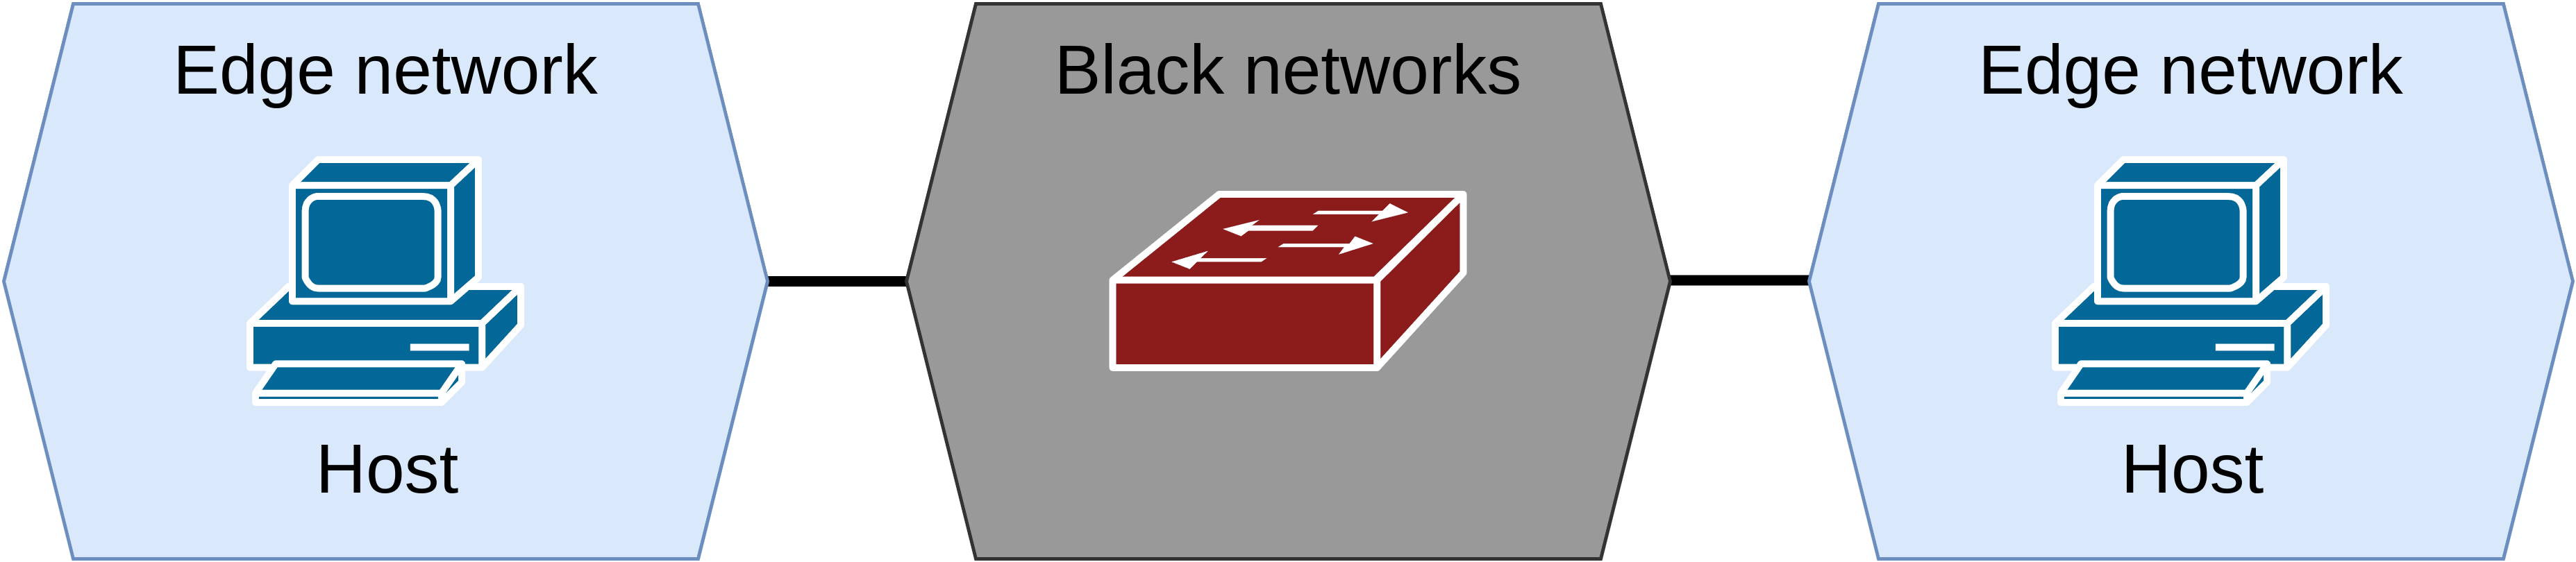
\includegraphics[width=8cm]{images/chapter_4/network_model.png}
    \caption[Network model]{Our network model showing the separation of trusted \gls{edgenetwork}s and semi-trusted \gls{blacknetwork}s. While \gls{edgenetwork}s are the source and target of our network slice traffic, \gls{blacknetwork}s act as transit networks. There can be multiple \gls{blacknetwork}s between our \gls{edgenetwork}s, but for simplicity reasons only one of them is indicated in the figure.}
    \label{fig:network_model}
\end{figure}

\paragraph{Edge networks}
are the origin and target of one specific network slice. Each \gls{edgenetwork} is partially trusted by us, because we or another trusted party operate the core infrastructure. We only expect threats from adversaries outside of our switches or slicing architecture following a \gls{zerotrust} approach, for example as a host established within our \gls{edgenetwork}.

\paragraph{Black networks}
lie between the \gls{edgenetwork}s and are operating under a service level agreement (\acrshort{sla}). There may be any number of \gls{blacknetwork}s between two edges, including none. A \gls{blacknetwork} acts as a transit network to us and is semi-trusted because the infrastructure is not operated by us. We do trust that the \gls{blacknetwork} will act according to protocol, but it might be interested in breaking confidentiality or even integrity. As with our \gls{edgenetwork}s, we expect attackers to be established outside of the switching and slicing architecture following a \gls{zerotrust} approach, apart from potential eavesdropping or integrity violation attempts by the transport infrastructure of the \gls{blacknetwork}.

Please note that one specific network may play different roles for different network slices. One slice may pass through a \gls{blacknetwork} that is also the origin (and thus \gls{edgenetwork}) of another slice.

Our network model can also be seen in Figure \ref{fig:network_model}.


\section{Protection Goals}
\label{protection_goals}
The next question we posed was what we actually desire to protect from our attackers. In general we strive to protect the communication from one host to another and provide certain guarantees to the hosts. These guarantees include \gls{bandwidth}, \gls{latency}, \gls{jitter}, \gls{lossrate} and of course availability. Furthermore we want to protect traffic from modification or information disclosure in networks between our \gls{edgenetwork}s. We do not require this protection on our \gls{edgenetwork}s, since we trust our self-managed infrastructure to a certain degree. Our protection goals are thus:
\begin{description}[style=multiline, labelwidth=0.7cm]
    \item[\namedlabel{P1}{P1}] \textbf{Confidentiality} Traffic needs to be protected from disclosure outside of the \gls{edgenetwork}s.
    \item[\namedlabel{P2}{P2}] \textbf{Integrity} Traffic needs to be protected from modification by attackers outside of our path on the \gls{edgenetwork}s and from attackers on the \gls{blacknetwork}.
    \item[\namedlabel{P3}{P3}] \textbf{Availability} Slices need to be available for communication and deliver packets to the recipient at all times during their lifespan.
    \item[\namedlabel{P4}{P4}] \textbf{Resilience} Slices need to provide their guaranteed network resources with their specified \gls{bandwidth}, \gls{latency}, \gls{jitter} and \gls{lossrate}, even when the network is under attack.
\end{description}


\section{Threats and Attackers}
\label{adversaries}
Now that we specified our protection goals, the attackers should be designed.

As previously mentioned, Ruxandra Olimid et. al \cite{SE2} classified threats to network slicing as either life-cycle threats, inter-slice threats or intra-slice threats. We will present our attackers for these threats below.

\paragraph{Inter-slice threats} For inter-slice threats we will create an attacker utilizing a lot of resources within another slice to overload the network and potentially create artifacts in our slice that should be prevented. We do not consider side-channel attacks on our slicing implementation to test the isolation between slices as it heavily depends on the used components while we will try to support a variety of components (e.g. the implementation of queues in the linux kernel vs a hardware switch).

\paragraph{Life-cycle threats} For life-cycle threats we will introduce two attackers, one spamming our application plane with arbitrary requests and one spamming our slice coordinators with valid requests. We hope to achieve denial of service for new slice registrations with the first attacker and an overload of network resources by the second attacker.

\paragraph{Intra-slice threats} As the last two attackers we will consider attackers attempting to eavesdrop or violate integrity within one of the \gls{blacknetwork}s between our two \gls{edgenetwork}s. The eavesdropping attacker will only observe traffic attempting to break confidentiality. The integrity attacker will however try to replay and craft new messages (including sending modified packets additionally). Dropping and modifying packets should not be supported by the attacker, as we can not compensate for the subsequently lost packets while only using a single path without resending packets, potentially violating resource guarantees. Eavesdroppers and integrity attackers are not expected on our \gls{edgenetwork}s, as we trust our local environment infrastructure (but not all tenants).

\paragraph{Exclusions} As it has already been the case with the attacker on integrity, we do not consider active in-path attackers (apart from the integrity attacker), as they could disrupt communication at any time. If resilience against these kinds of attacks is needed, the solution would need to be extended to include multiple paths. This is however out of scope for this thesis. Apart from all components and links used by the network slice, in-path attackers contain our entire application plane, as any component of the application plane that participates in a slice could instruct other components to disrupt the connection or disrupt the connection themselves. To compensate this, routing via multiple alternative paths would be required, introducing redundancy to the network.

We also do not include attackers on confidentiality and integrity on the application plane here, as this could be easily solved by using transport layer security (TLS) enabled protocols for communication in the future, which is however also currently out of scope for this thesis. The same applies to a proper authentication scheme on the application plane.

There are also no attackers on our control plane, because all control plane components are in-path (as stated above) and are not directly reachable by tenant devices of our networks that we distrust.

\paragraph{} Our attacker definitions are thus as follows:
\begin{description}[style=multiline, labelwidth=0.7cm]
    \item[\namedlabel{A1}{A1}] \textbf{Slice availability and resilience} Overloads the network by sending a lot of traffic through another slice that has shared components and network links with our slice that should be protected. Attacks protection goals \ref{P3} (availability) and \ref{P4} (resilience).
    \item[\namedlabel{A2}{A2}] \textbf{Application plane availability and resilience (1)} Spams invalid slice requests on the exposed application plane components attempting to disrupt the creation of new slices. Attacks protection goals \ref{P3} (availability) and \ref{P4} (resilience).
    \item[\namedlabel{A3}{A3}] \textbf{Application plane availability and resilience (2)} Spams valid authenticated slice requests on the exposed application plane components attempting to overload the network by capacity or frequent slice creation and removal. Attacks protection goals \ref{P3} (availability) and \ref{P4} (resilience).
    \item[\namedlabel{A4}{A4}] \textbf{Slice confidentiality} Attempts to eavesdrop within one of the \gls{blacknetwork}s. Attacks protection goal \ref{P1} (confidentiality).
    \item[\namedlabel{A5}{A5}] \textbf{Slice integrity} Attempts to modify contents of a slice within one of the \gls{blacknetwork}s by replaying or sending additional packets. Will not modify or drop packets, but may send modified packets as additional packets. Attacks protection goal \ref{P2} (integrity).
\end{description}

Our attackers can also be seen in Figure \ref{fig:attacker_model}.

%\begin{landscape}
    \begin{figure}[h]
        \centering
        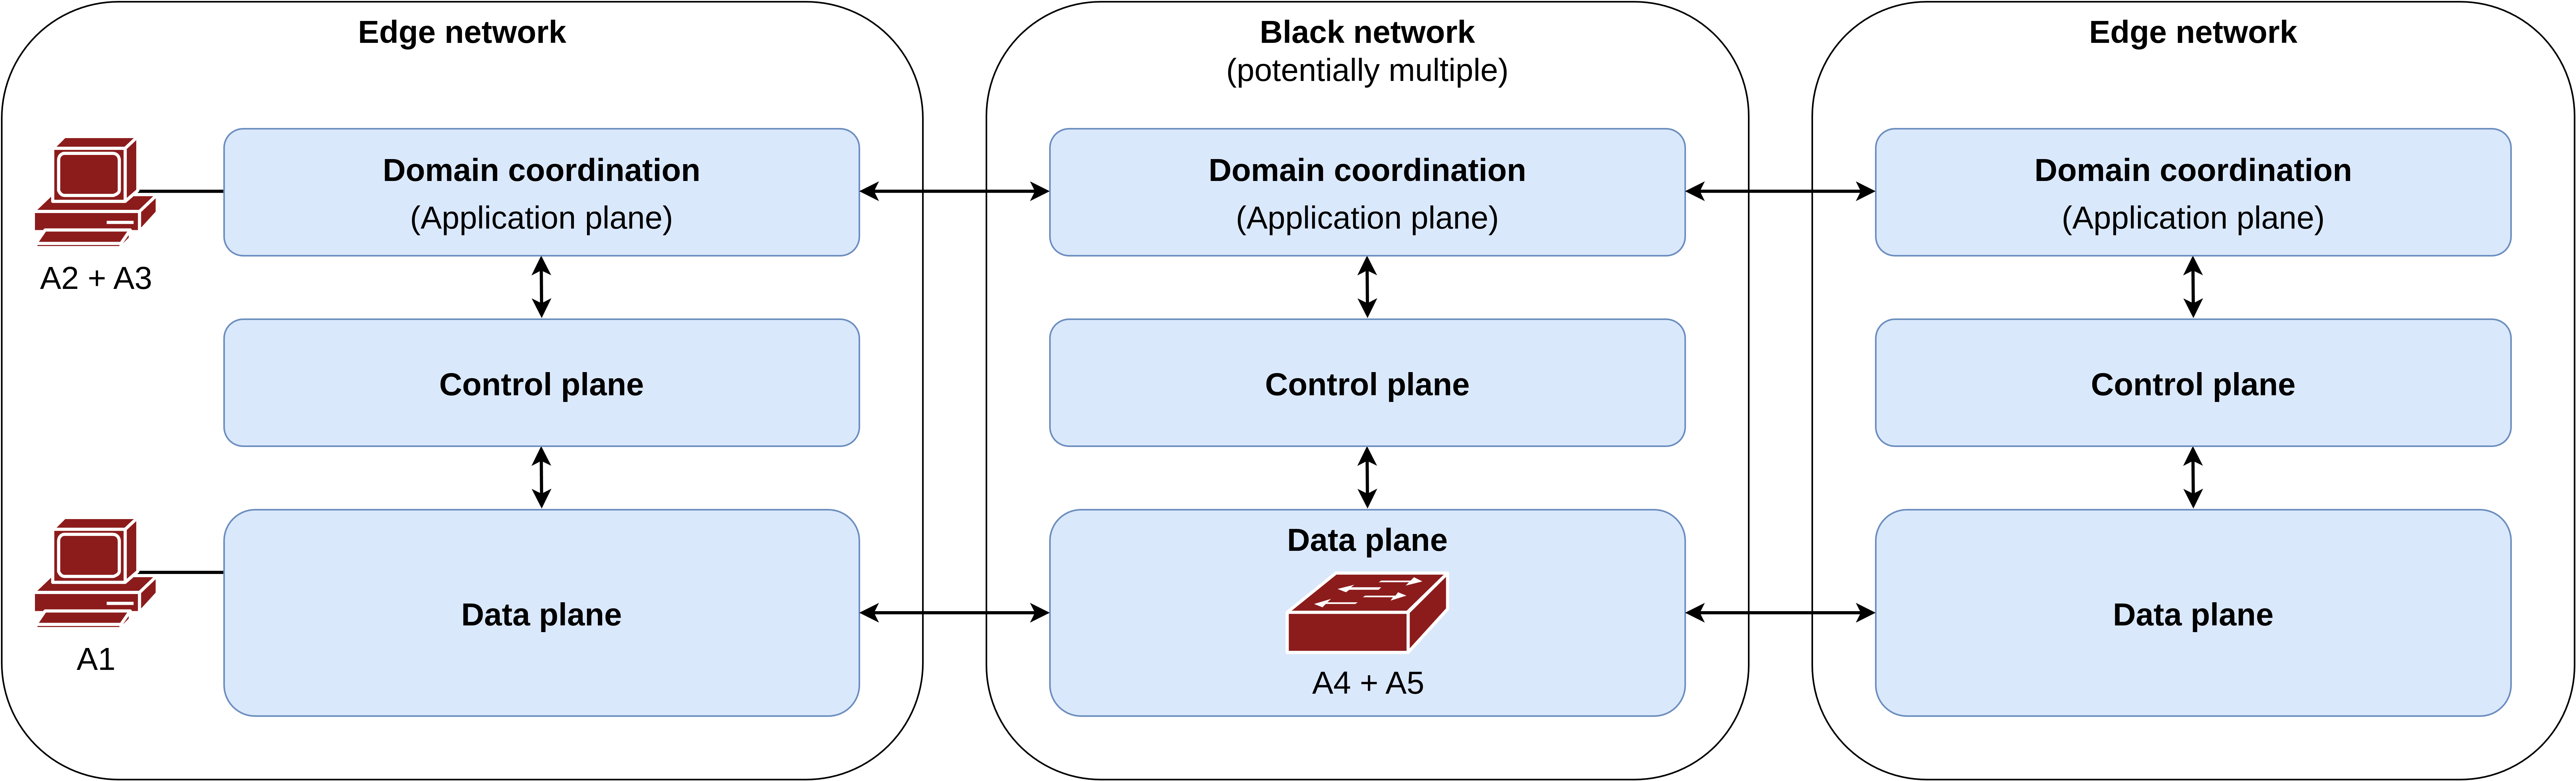
\includegraphics[width=\linewidth]{images/chapter_4/attacker_model.png}
        \caption[Attacker model]{Our attacker model indicating their location per domain and \acrshort{sdn} plane.}
        \label{fig:attacker_model}
    \end{figure}
%\end{landscape}
\chapter{Design}
\label{design}
\iffalse
\begin{itemize}
    \item Components
    \begin{itemize}
        \item Overview
        \item ESMF \& CTMF
        \item DSMF \& DTMF
        \item Controller
        \item SDN Switch
        \item VPN Gateway
    \end{itemize}
    \item Concepts
    \begin{itemize}
        \item Distributed trust and authority
        \item State synchronization (2PCP)
        \item Strict separation of SDN layers
    \end{itemize}
\end{itemize}
\fi
This chapter is centered around the components and concepts embodied in our network slicing architecture. We will first give an overview over our components and then present some concepts that will need to be implemented by our implementation.

\section{Components}
In order to present our components to achieve a network slicing architecture, we will group them by SDN layer. We will begin by inspecting the data plane, followed by the control plane and conclude with the application plane. In figure [LINK] you can already see the final result of our suggested topology, where the links that are used by the slice are marked green. Please note that other network architectures are possible as well and this is only an example topology. The focus is on the application and control plane components per network domain. All components below are virtual network functions (VNFs).

The presented components are partially sourced from Fuhrberg et al. \cite{SE4}. Our contribution is the addition of specialized components for the black network, the redesign of logic on each of the components for our new distributed slice management approach and for the other concepts introduced in section \ref{design_concepts}.

\subsection{Data plane}
The job of the data plane is to transport traffic, so in our use case it will need to achieve the network resource isolation we require from our slices (protection goal \hyperref[P4]{P4}). To configure this isolation we need a way to assign traffic to QoS flows that span from one edge to another, traversing all required black networks in the process. Furthermore we need to limit third party traffic so it may not impede our resource allocations. In order to perform easier routing decisions along our path, we wish to label traffic traversing a network slice according to the MPLS scheme. As a last data plane measure we require traffic to be encrypted and protected against modification while traversing the black networks (protection goal \hyperref[P1]{P1} and \hyperref[P2]{P2}).

To deploy the QoS flows and secure them against third party traffic (protection goal \hyperref[P4]{P4}), we will need to make use of SDN switches. The switches will forward the packets from source to destination. While the first switch will tag the packets with an MPLS label to facilitate easier routing and perform authentication of slice traffic along the entire path, the last switch will finally remove the MPLS label again. All switches will discard MPLS traffic from different ports than expected and drop packets with MPLS labels not expected to be found on a port. This way we can prevent third party traffic entering our slice, protecting the integrity of our slice [LINK].

The switches also have to limit traffic from other participants to guarantee the slice resources, which can be realised by creating a "default slice" for all non-slice traffic on the network. This can lead to underprovisioning of network resources however. The default slice should be shrunk when new slices are created to accommodate the new slices or have a relatively small size to not be able to disturb our slices. The slice resources can be guaranteed by setting up queues for all slices and the default slice to limit the overall possible outgoing traffic per port. For ingress traffic on ports, port ingress limits should be set up so that the switch may not be overloaded by the sheer amount of traffic from all sides.

For the encryption along the black networks we will use VPN gateways that encrypt traffic (protection goal \hyperref[P1]{P1}). The VPN gateways will only ever see traffic from slices and should be shielded from all other traffic to limit the surface of attack. To connect to a remote end, VPN gateways will use tunnels that need to be cryptographically secure to not disclose information and have protection against data manipulation to protect our data integrity (protection goal \ref{P2}). In order to limit the effect of information disclosure by the sheer existence of a slice through the black networks, we will bundle multiple slices through one single tunnel. Packets from the tunnel will be tagged with another tunnel MPLS label by the first switch and the label will be removed again by the final tunnel switch due to the same reasons as with the original slice packets (integrity). A packet is assigned to a specific tunnel by examining the slice id in the MPLS label from the first slice switch.

%By tagging the packets with an MPLS label again and using the changing MPLS labels for routing, we effectively build a service function chain (SFC) to the destination host (via the two VPN gateways), which partially anonymizes the recipient to the black networks.

When a packet is traversing the tunnel, the unified guarantees for the individual slices should apply, meaning a sum of the individual bandwidths and the lowest values for latency, jitter and loss.

% TODO: Mention that tunnel needs integrity protection above with protection goal 1 -> add 2 - maybe mention wireguard already?

The last required components on the data plane are the hosts that wish to send or receive data via the slices. One of these hosts should contact the application plane to create a new slice before initiating communications with the remote host.

% TODO - Figure for only the data plane components?

\subsection{Control plane}
The control plane should mainly support deploying our rules to our devices. Creating the flows is supported by using OpenFlow through a standard SDN controller. For our queues and ingress limits we will need a separate service realizing them on the switches though, as these features are not currently supported by OpenFlow. We suggest implementing them via a service running on the SDN switches. For the VPN gateways we require another service running on the specialized VPN gateway hosts allowing us to register, resize and delete tunnels, as well as assigning slices to tunnels.

% TODO - Figure for only the control plane components?

\subsection{Application plane}
The application plane will then care about defining the rules that should be deployed. In order to instruct the control plane, we will create one infrastructure coordinator per domain that will carry out all infrastructure tasks. This service that we will call a domain slice management function (DSMF) will know about the entire topology and will have the routing information to other domains. It will set up domains and tunnels on the local infrastructure if requested and specify upfront whether resources can be guaranteed or not. This service thus follows an IntServ pattern to realize network slices.

Apart from this infrastructure service we will need to establish a domain coordination service, called an edge slice management function (ESMF). The ESMF will be used to coordinate the deployment of slices and tunnels across multiple domains. Apart from the coordination role it should also be the main endpoint for participants from the local domain to request slices through the network. By contacting other domains and the local infrastructure service the coordination service can evaluate whether a slice request from a participant is currently possible or not. For isolation purposes, only the coordination service of a domain (ESMF) will be allowed to contact the infrastructure service (DSMF) of the same domain. The ESMFs will only talk between each other and with tenants of their own domain.

While ESMF and DSMF allow the creation of slices and tunnels on their respective domain, versions of them also exist with reduced functionality for black networks that do not wish to offer their tenants slice support. The ESMF will be replaced with a core tunnel management function (CTMF) and the DSMF will be replaced with a domain tunnel management function (DTMF). A CTMF will never initiate a new tunnel but rather receive tunnel requests from coordinating ESMFs. Also a CTMF will never accept slice requests from tenants of their domain. They will thus only talk to an ESMF of another domain to coordinate new tunnels or with their own DTMF to deploy tunnels to their infrastructure and to check for resource availability. A CTMF may only talk to a DTMF and an ESMF may only talk to a DSMF, depending on the network role. CTMF and DTMF may only be deployed on black networks that are exclusively black networks, requiring their network domain to never be the beginning nor the end of a slice.

% TODO - Figure for only the application plane components?

\paragraph{} After joining the different SDN layers we thus reach our design topology (see figure [LINK]) that has the separation of different virtual network functions (VNFs) in mind.

% TODO - Figure of all layers

\section{Concepts}
\label{design_concepts}
After we presented our components we now want to mention our concepts behind certain design decisions, beginning with our concept of distributed trust and authority, our state synchronization and the strict separation of SDN layers.

\subsection{Distributed trust and authority}
Distributed trust and authority is one of our core requirements (see \hyperref[R2]{requirement R2}). While wanting to lend resources to participants of our and other networks participating in our slicing architecture and guaranteeing those resources to them, we do not want others taking deployment or infrastructure decisions for our local domain. This is why we separated the coordination across all domains and only expose the coordinators to the other domains. This way another domain can ask us to allocate resources for a new slice but we may deny the creation at any point in time. Still other domains can request slices and tunnels this way without having direct access or knowledge about our infrastructure.

\subsection{State synchronization}
In order to be able to coordinate slices and tunnels across multiple domains we need to synchronize a partial global state across them. Without this synchronization slices could potentially be deployed only in part, violating our requirement of the basic availability of a slice (see requirement \hyperref[R1]{R1} and protection goal \hyperref[P3]{P3}) when traffic can not pass all domains along the slice. We thus require to synchronize a global state for each slice between the coordinators.

We will realize this by leveraging the two-phase commit protocol (2PCP) \cite{2pcp}. This way tunnel and slices will first be reserved throughout the network and if all reservations succeeded they can then be deployed. A failure of the coordinating ESMF or a participant during the commit phase is no critical issue to us, as the host will not get a positive reply for the slice registration then. We do not guarantee the creation of slices to our tenants, but rather guarantee that a registered slice performs according to specification. Of course the issue could arise, that partially created slices persist on the network this way, but those dangling components could also be removed afterwards, when the system recovers from a failure.

\subsection{Strict separation of SDN layers}
In order to reach our goal to be relatively hardware independent (requirement \hyperref[R3]{R3}) we want to clearly structure our services according to our SDN layers. Of course this may not always be possible because for example our switch queue and ingress limit service will be vendor specific due to no unified API being available at this point to manage these characteristics. For all other services, the design has been separated according to the SDN layers to be able to swap out different components of the SDN environment with ease. For example to use a switch of a different vendor, only the switch queue and ingress limit service will need to be implemented for this vendor while the rest of the components can remain in use. This includes the integration of hardware switches or servers, enabling our topology to be executed outside of testbench scenarios.
\chapter{Implementation}
\label{implementation}

In this chapter we are going to be more specific about the details of our implementation that we produced from our design. At first, we will state our virtual network function (\acrshort{vnf}) specifications, before describing some details about our components, the realization of our previously mentioned concepts and challenges we faced while implementing.


\section{Specification}
\label{impl_specification}
In this section we will focus on our specifications. First we will present our protocol specifications for each \acrshort{vnf}, before providing communication examples to create and remove a slice.

\subsection{OpenAPI specifications}
To interconnect our \acrshort{vnf}s, we use multiple \acrshort{rest} \acrshort{api}s. Our \acrshort{rest} protocol specifications are conveniently provided via \Gls{openapi} descriptions \cite{openapi}. \Gls{openapi} is a project unifying the specification of web protocols by providing protocol descriptions in either JSON or YAML format. This way, our and future implementations of our protocols can auto-generate code to communicate with our services by using the \Gls{openapi} generator project \cite{openapi-generator}. \Gls{openapi} generators take a protocol description and convert them to something else. This can be client or server implementations written in various programming languages. There are also other projects providing support to present the specifications in human-readable form to developers, such as SwaggerUI \cite{swaggerui} or Redocly \cite{redocly}.

We provide \Gls{openapi} specifications for each service required by our design. The specifications can be found at the end of this thesis (see Appendix \ref{specifications}) in human-readable form, or in the accompanying sources in JSON format. We chose to unify the implementations of \acrshort{esmf} and \acrshort{ctmf}, as well as the implementations of \acrshort{dsmf} and \acrshort{dtmf} though, because their implementations are identical apart from enabling or disabling certain functionality.

The basic endpoints of each component can be seen in the tables \ref{table:esmf} through \ref{table:vpn_gateway}. Further details on parameters and responses can be found at the end of this thesis in Appendix \ref{specifications}.

All \acrshort{vnf}s provide endpoints for authentication (apart from the \acrshort{sdn} controller). This is currently just a placeholder to establish a real authentication scheme later. In the current specification the authentication endpoint takes no parameters and returns a predefined token. All the other endpoints then take this token to authorize requests. The details on how these endpoints work together can then be seen in Section \ref{impl_communication}, where we take a closer look on the creation and removal of a slice.

\begin{table}[htp]
    \begin{tabularx}{\textwidth}{ |l|X| }
        \hline
        \textbf{Endpoint}       & \textbf{Description}                                                                                \\
        \hline
        /v1/auth                & Endpoint that can be contacted by all parties to authenticate and obtain a new authentication token \\
        /v1/configuration       & Endpoint to configure this service                                                                  \\
        \hline
        /v1/slice               & Endpoint that can be contacted by hosts to submit new slice requests                                \\
        \hline
        /v1/slice\_reservation  & Endpoint used by other \acrshort{esmf}s to reserve a slice                                          \\
        /v1/slice\_deployment   & Endpoint used by other \acrshort{esmf}s to deploy a slice                                           \\
        /v1/tunnel\_reservation & Endpoint used by other \acrshort{esmf}s to reserve a tunnel                                         \\
        /v1/tunnel\_deployment  & Endpoint used by other \acrshort{esmf}s to deploy a tunnel                                          \\
        \hline
    \end{tabularx}
    \caption[\acrshort{esmf} endpoints]{The endpoints of our \acrshort{esmf} implementation alongside their functionality.}
    \label{table:esmf}
\end{table}

\begin{table}[htp]
    \begin{tabularx}{\textwidth}{ |l|X| }
        \hline
        \textbf{Endpoint}       & \textbf{Description}                                                                                \\
        \hline
        /v1/auth                & Endpoint that can be contacted by all parties to authenticate and obtain a new authentication token \\
        /v1/configuration       & Endpoint to configure this service                                                                  \\
        \hline
        /v1/tunnel\_reservation & Endpoint used by \acrshort{esmf}s to reserve a tunnel                                               \\
        /v1/tunnel\_deployment  & Endpoint used by \acrshort{esmf}s to deploy a tunnel                                                \\
        \hline
    \end{tabularx}
    \caption[\acrshort{ctmf} endpoints]{The endpoints of our \acrshort{ctmf} implementation alongside their functionality. Includes a subset of the \acrshort{esmf} endpoints.}
    \label{table:ctmf}
\end{table}

\begin{table}[htp]
    \begin{tabularx}{\textwidth}{ |l|X| }
        \hline
        \textbf{Endpoint}       & \textbf{Description}                                                                                \\
        \hline
        /v1/auth                & Endpoint that can be contacted by all parties to authenticate and obtain a new authentication token \\
        /v1/configuration       & Endpoint to configure this service                                                                  \\
        \hline
        /v1/slice\_reservation  & Endpoint used by our \acrshort{esmf} to reserve a slice                                             \\
        /v1/slice\_deployment   & Endpoint used by our \acrshort{esmf} to deploy a slice                                              \\
        /v1/tunnel\_reservation & Endpoint used by our \acrshort{esmf} to reserve a tunnel                                            \\
        /v1/tunnel\_deployment  & Endpoint used by our \acrshort{esmf} to deploy a tunnel                                             \\
        \hline
    \end{tabularx}
    \caption[\acrshort{dsmf} endpoints]{The endpoints of our \acrshort{dsmf} implementation alongside their functionality.}
    \label{table:dsmf}
\end{table}

\begin{table}[htp]
    \begin{tabularx}{\textwidth}{ |l|X| }
        \hline
        \textbf{Endpoint}       & \textbf{Description}                                                                                \\
        \hline
        /v1/auth                & Endpoint that can be contacted by all parties to authenticate and obtain a new authentication token \\
        /v1/configuration       & Endpoint to configure this service                                                                  \\
        \hline
        /v1/tunnel\_reservation & Endpoint used by our \acrshort{esmf} to reserve a tunnel                                            \\
        /v1/tunnel\_deployment  & Endpoint used by our \acrshort{esmf} to deploy a tunnel                                             \\
        \hline
    \end{tabularx}
    \caption[\acrshort{dtmf} endpoints]{The endpoints of our \acrshort{dtmf} implementation alongside their functionality. Includes a subset of the \acrshort{dsmf} endpoints.}
    \label{table:dtmf}
\end{table}

\begin{table}[htp]
    \begin{tabularx}{\textwidth}{ |l|X| }
        \hline
        \textbf{Endpoint} & \textbf{Description}                                                                                \\
        \hline
        /v1/auth          & Endpoint that can be contacted by all parties to authenticate and obtain a new authentication token \\
        \hline
        /v1/queue         & Endpoint used to manage \acrshort{qos} queues on this switch                                        \\
        /v1/policy        & Endpoint used to manage traffic shaping on ingress ports of this switch                             \\
        \hline
    \end{tabularx}
    \caption[Switch endpoints]{The endpoints of our switch implementation alongside their functionality.}
    \label{table:switch}
\end{table}

\begin{table}[htp]
    \begin{tabularx}{\textwidth}{ |l|X| }
        \hline
        \textbf{Endpoint}    & \textbf{Description}                                                           \\
        \hline
        /stats/switches      & Endpoint used to list all switches connected to the \acrshort{sdn} controller. \\
        /stats/desc          & Endpoint used to obtain information on a specific switch                       \\
        \hline
        /stats/flow          & Endpoint used to fetch flow stats from a specific switch                       \\
        /stats/flowentry     & Endpoint used to manage flows on a switch                                      \\
        /stats/tablefeatures & Endpoint used to retrieve details and all features of a flow table on a switch \\
        /stats/portdesc      & Endpoint used to obtain port lists and descriptions of a switch                \\
        /stats/queue         & Endpoint used to view available queues on a switch                             \\
        \hline
    \end{tabularx}
    \caption[Controller endpoints]{The endpoints of our \acrshort{sdn} controller implementation. Some endpoints contain additional sub-endpoints under their path that have been left out for simplicity. Please refer to the specification at the end of this thesis for additional details. This \acrshort{api} is a subset of the RYU \acrshort{rest} \acrshort{api} \cite{ryu-rest}.}
    \label{table:controller}
\end{table}

\begin{table}[htp]
    \begin{tabularx}{\textwidth}{ |l|X| }
        \hline
        \textbf{Endpoint} & \textbf{Description}                                                                                \\
        \hline
        /v1/auth          & Endpoint that can be contacted by all parties to authenticate and obtain a new authentication token \\
        \hline
        /v1/tunnel\_entry & Endpoint used to manage tunnel entries on this \acrshort{vpn} gateway                               \\
        \hline
    \end{tabularx}
    \caption[\acrshort{vpn} gateway endpoints]{The endpoints of our \acrshort{vpn} gateway implementation alongside their functionality.}
    \label{table:vpn_gateway}
\end{table}

\subsection{Communication}
\label{impl_communication}
In this section we are going to describe the communication required for the creation and removal of a slice. Please note that the previously described authentication is being performed in advance and not described for every \acrshort{vnf}. In general all requests are authenticated and thus require a previous authentication request.

\subsubsection{Slice creation}
In order to create one or multiple slices, a host will contact the assigned \acrshort{esmf} of their domain. The host will submit the requirements for the slices to the \acrshort{esmf} and wait for a response.

For each slice the \acrshort{esmf} will then either assign an existing tunnel to the slice or create a new tunnel for the slice. The tunnel will be created in a way, that all slices required to take the tunnel will fit in the tunnel. In the current implementation the \acrshort{esmf} will create one tunnel per source and target domain pair, so all slices sharing the same source and destination will take one tunnel. The \acrshort{esmf} will then attempt to push the new or adapted tunnel to the network, before pushing the slice to the network.

To push slice or tunnel parts to other networks, the corresponding network coordinators (\acrshort{ctmf} or other \acrshort{esmf}) are contacted. To perform the same actions on the local domain, the actions are forwarded to the local \acrshort{dsmf}. Every slice or tunnel that is being pushed first needs to be reserved with confirmation, before deploying it via the ID of the slice or tunnel. This way, the two-phase commit protocol is enacted according to our design. We first perform all required reservations. When all reservations are positive, we deploy everything and check whether the deployment was successful by collecting and checking all responses. If so, we report success back to the host. If not, we perform a removal of all reservations and deployments we made and report back a failure to the host.

While as previously mentioned the two-phase commit protocol can not recover from a failure of the coordinator, in this case the coordinating \acrshort{esmf}, we are still guaranteed to only report back success to the host when the slice has been fully deployed, which is our main goal with the synchronization as mentioned in the design before. When a participant fails while deploying the slice we still roll back. So only a failure of the coordinating \acrshort{esmf} while deploying slices or tunnels is a danger to us, because slice and tunnel components could remain on the system, blocking resources forever. This could potentially be mitigated in the future by creating startup sequences that remove detached network components when recovering from a failure. This is however currently not a priority of this thesis and thus subject to future work.

When slice or tunnel parts that need to be deployed are within a remote network, the \acrshort{ctmf} or \acrshort{esmf} of the remote network is instructed to carry out the tasks on their respective domain. A \acrshort{ctmf} will never obtain information on slices, but rather receive only the tunnel information (apart from tunnel keys). Currently, the instruction from the coordinating \acrshort{esmf} is simply forwarded to the \acrshort{dtmf} or \acrshort{dsmf} of the corresponding domain. This way the local requests as well as the remote requests end up on the infrastructure coordinators of the respective domains. Of course the forwarding \acrshort{esmf} and \acrshort{ctmf} can perform checks on these slice and tunnel requests.

So now as we synchronized state sufficiently, we can focus on the actual deployment of the components. As previously mentioned, the infrastructure coordinator (\acrshort{dtmf} or \acrshort{dsmf}) will receive reservations for slices or tunnels. These reservations are stored locally after checking for feasibility (whether resources are available considering all other deployments and reservations). Then we will either receive a deployment request or a removal request. If we receive a removal request, we simply drop the reservation. If we receive a deployment request, we contact the switches to create queues and ingress limits via a \acrshort{rest} \acrshort{api} (see Table \ref{table:switch}), the controller via another \acrshort{rest} \acrshort{api} (see Table \ref{table:controller}) to deploy our flows, and the \acrshort{vpn} gateways to deploy our tunnel entries and exits via yet another \acrshort{rest} \acrshort{api} (see Table \ref{table:vpn_gateway}). To get information about what is deployed per slice and tunnel, please have a look at Section \ref{impl_concepts}.

The entire process of creating a slice can also be seen in our three diagrams for the state synchronization (see Figure \ref{fig:slice_creation_synchronization}), the communication on the \gls{edgenetwork}s (see Figure \ref{fig:slice_creation_edge}) and on our \gls{blacknetwork}s (see Figure \ref{fig:slice_creation_bn}). Please note that the diagrams are based on using only one \gls{blacknetwork}. Of course multiple \gls{blacknetwork}s would be possible as well by repeating the communication to our \gls{blacknetwork} for every other \gls{blacknetwork}.

\newpage

\begin{figure}[H]
    \centering
    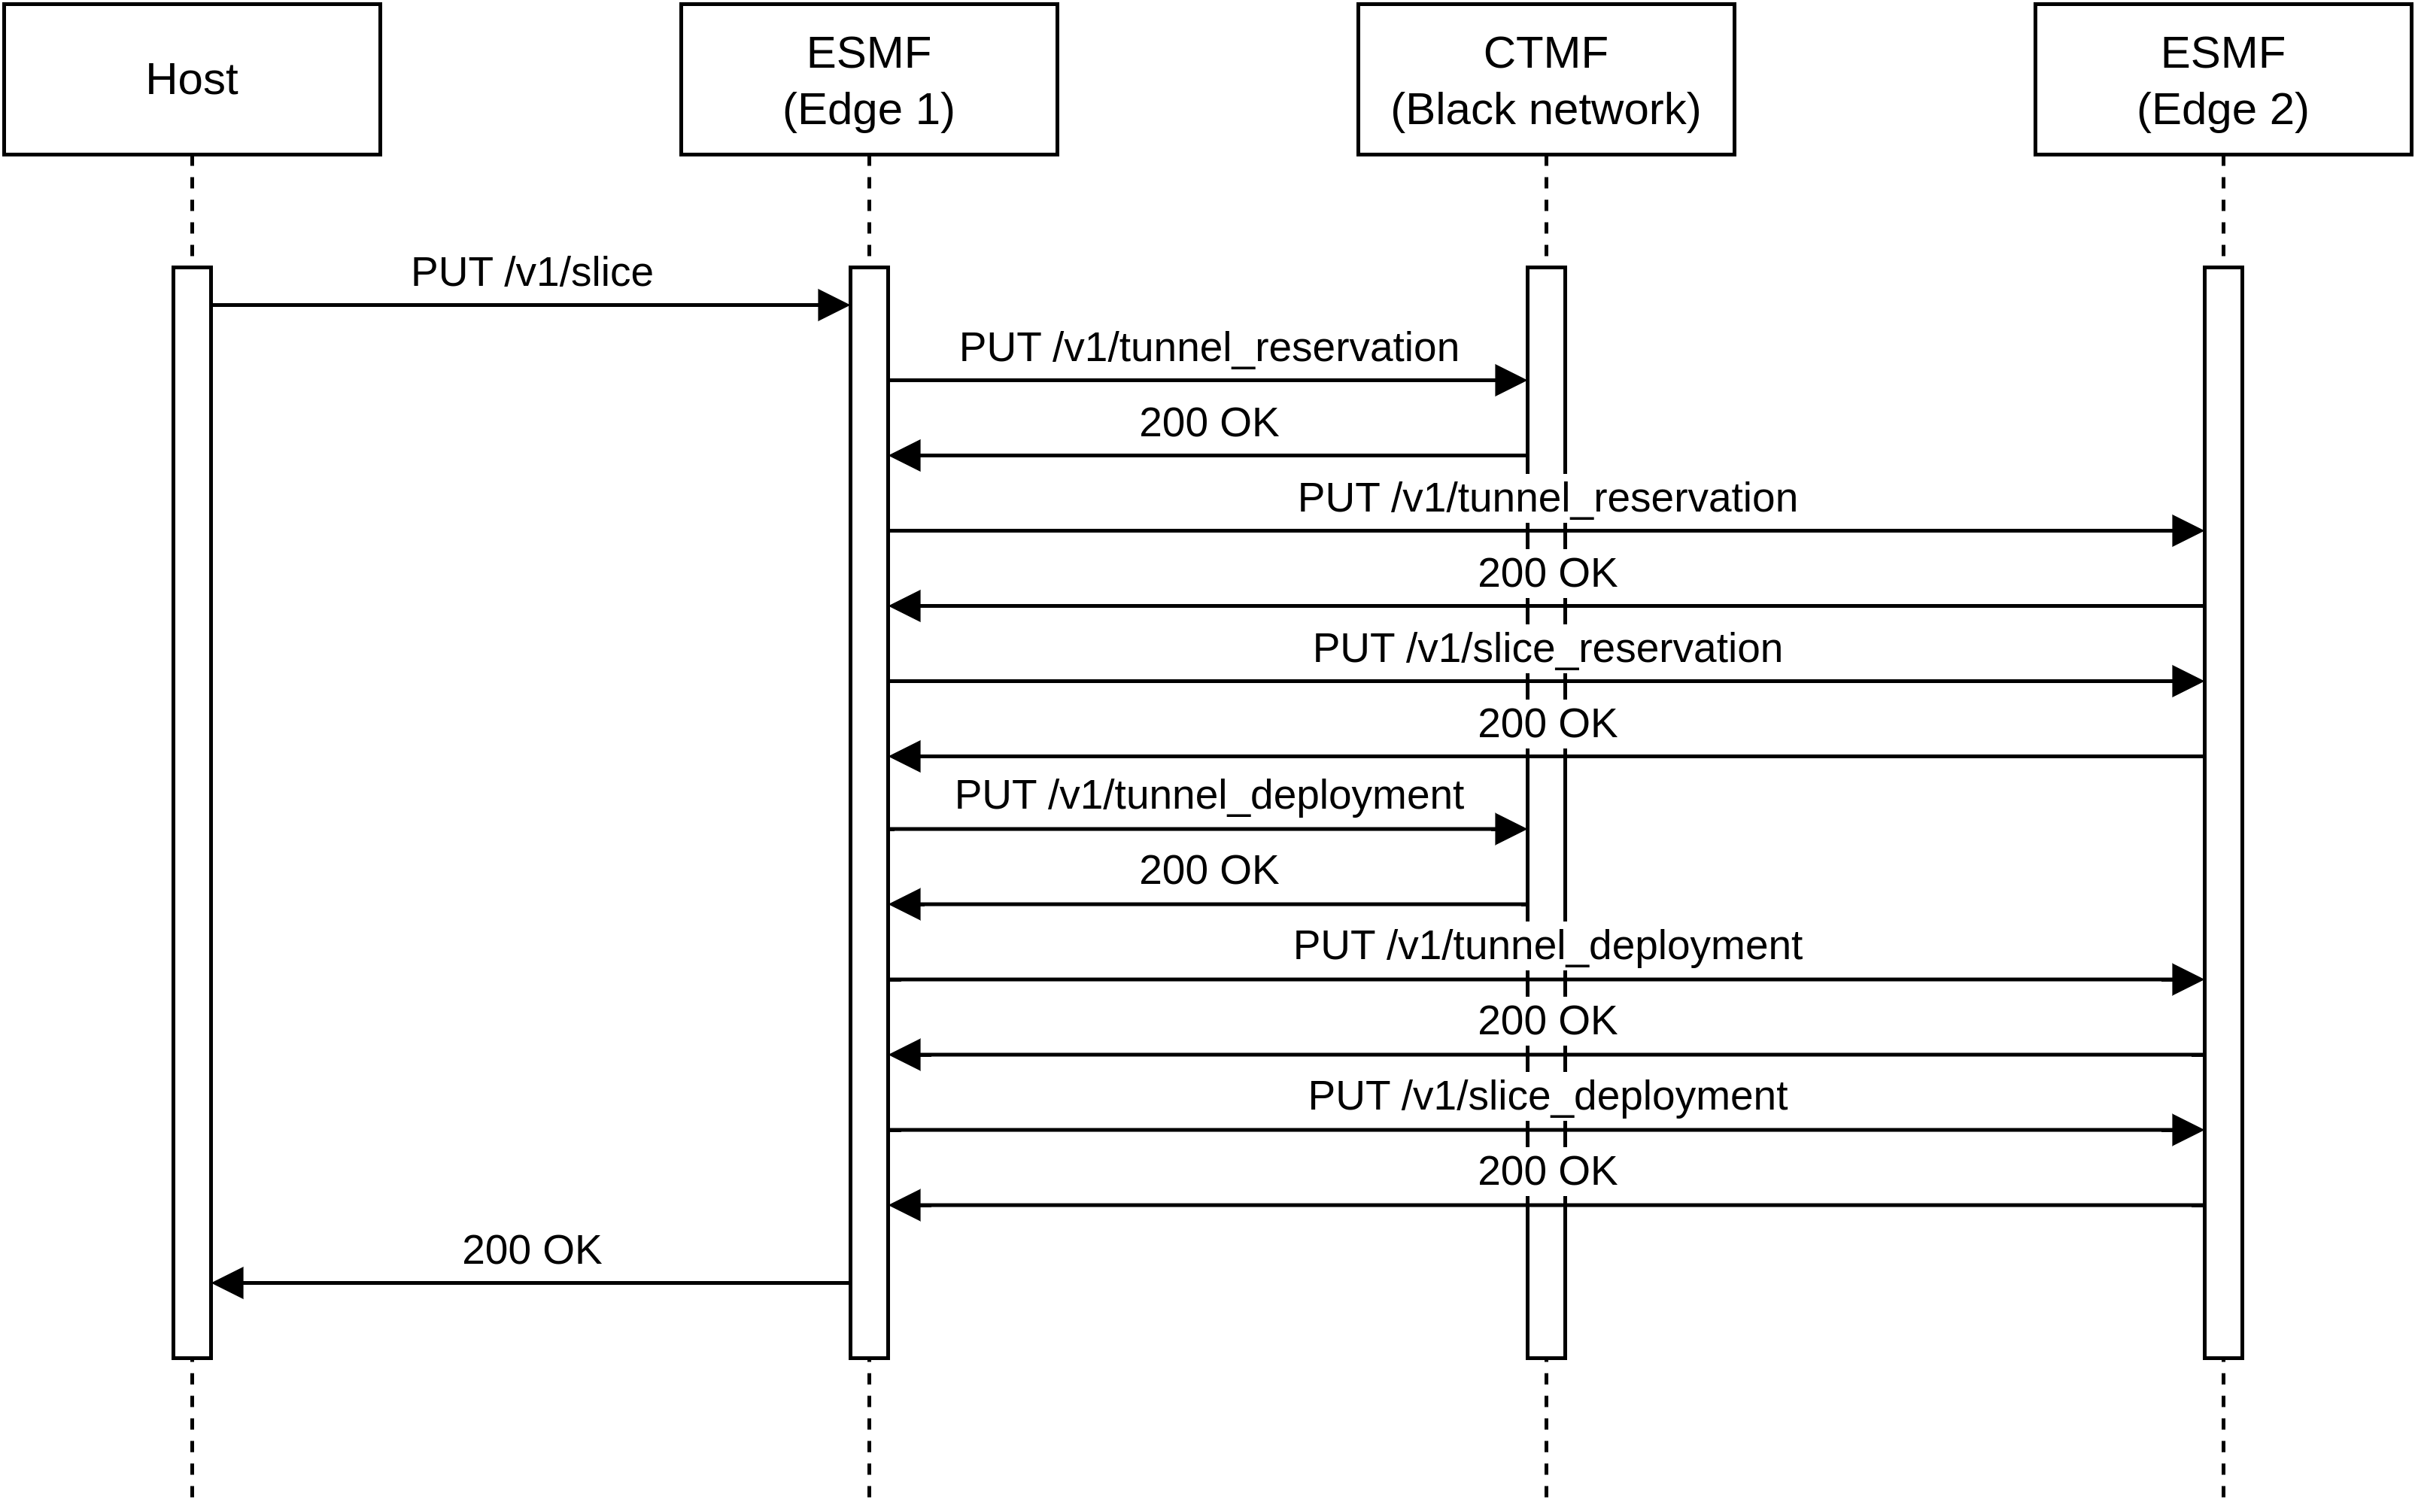
\includegraphics[width=\linewidth]{images/chapter_6/slice_creation_coordination.png}
    \caption[Slice creation on the coordinators]{Successful \acrshort{esmf} and \acrshort{ctmf} synchronization to create a slice illustrated in a sequence diagram. The coordinator \acrshort{esmf} that has been contacted by the host will contact all other domain coordinators to check whether the slice and the tunnel generated by the \acrshort{esmf} is feasible first, before instructing everyone to deploy. Finally the \acrshort{esmf} responds back to the coordinating host to indicate successful slice creation. If any steps fail, everything will be rolled back with removal requests and the host would receive a negative reply. If there is more than one \gls{blacknetwork}, the requests for the \acrshort{ctmf} need to be applied on each of them.}
    \label{fig:slice_creation_synchronization}
\end{figure}
\begin{figure}[H]
    \centering
    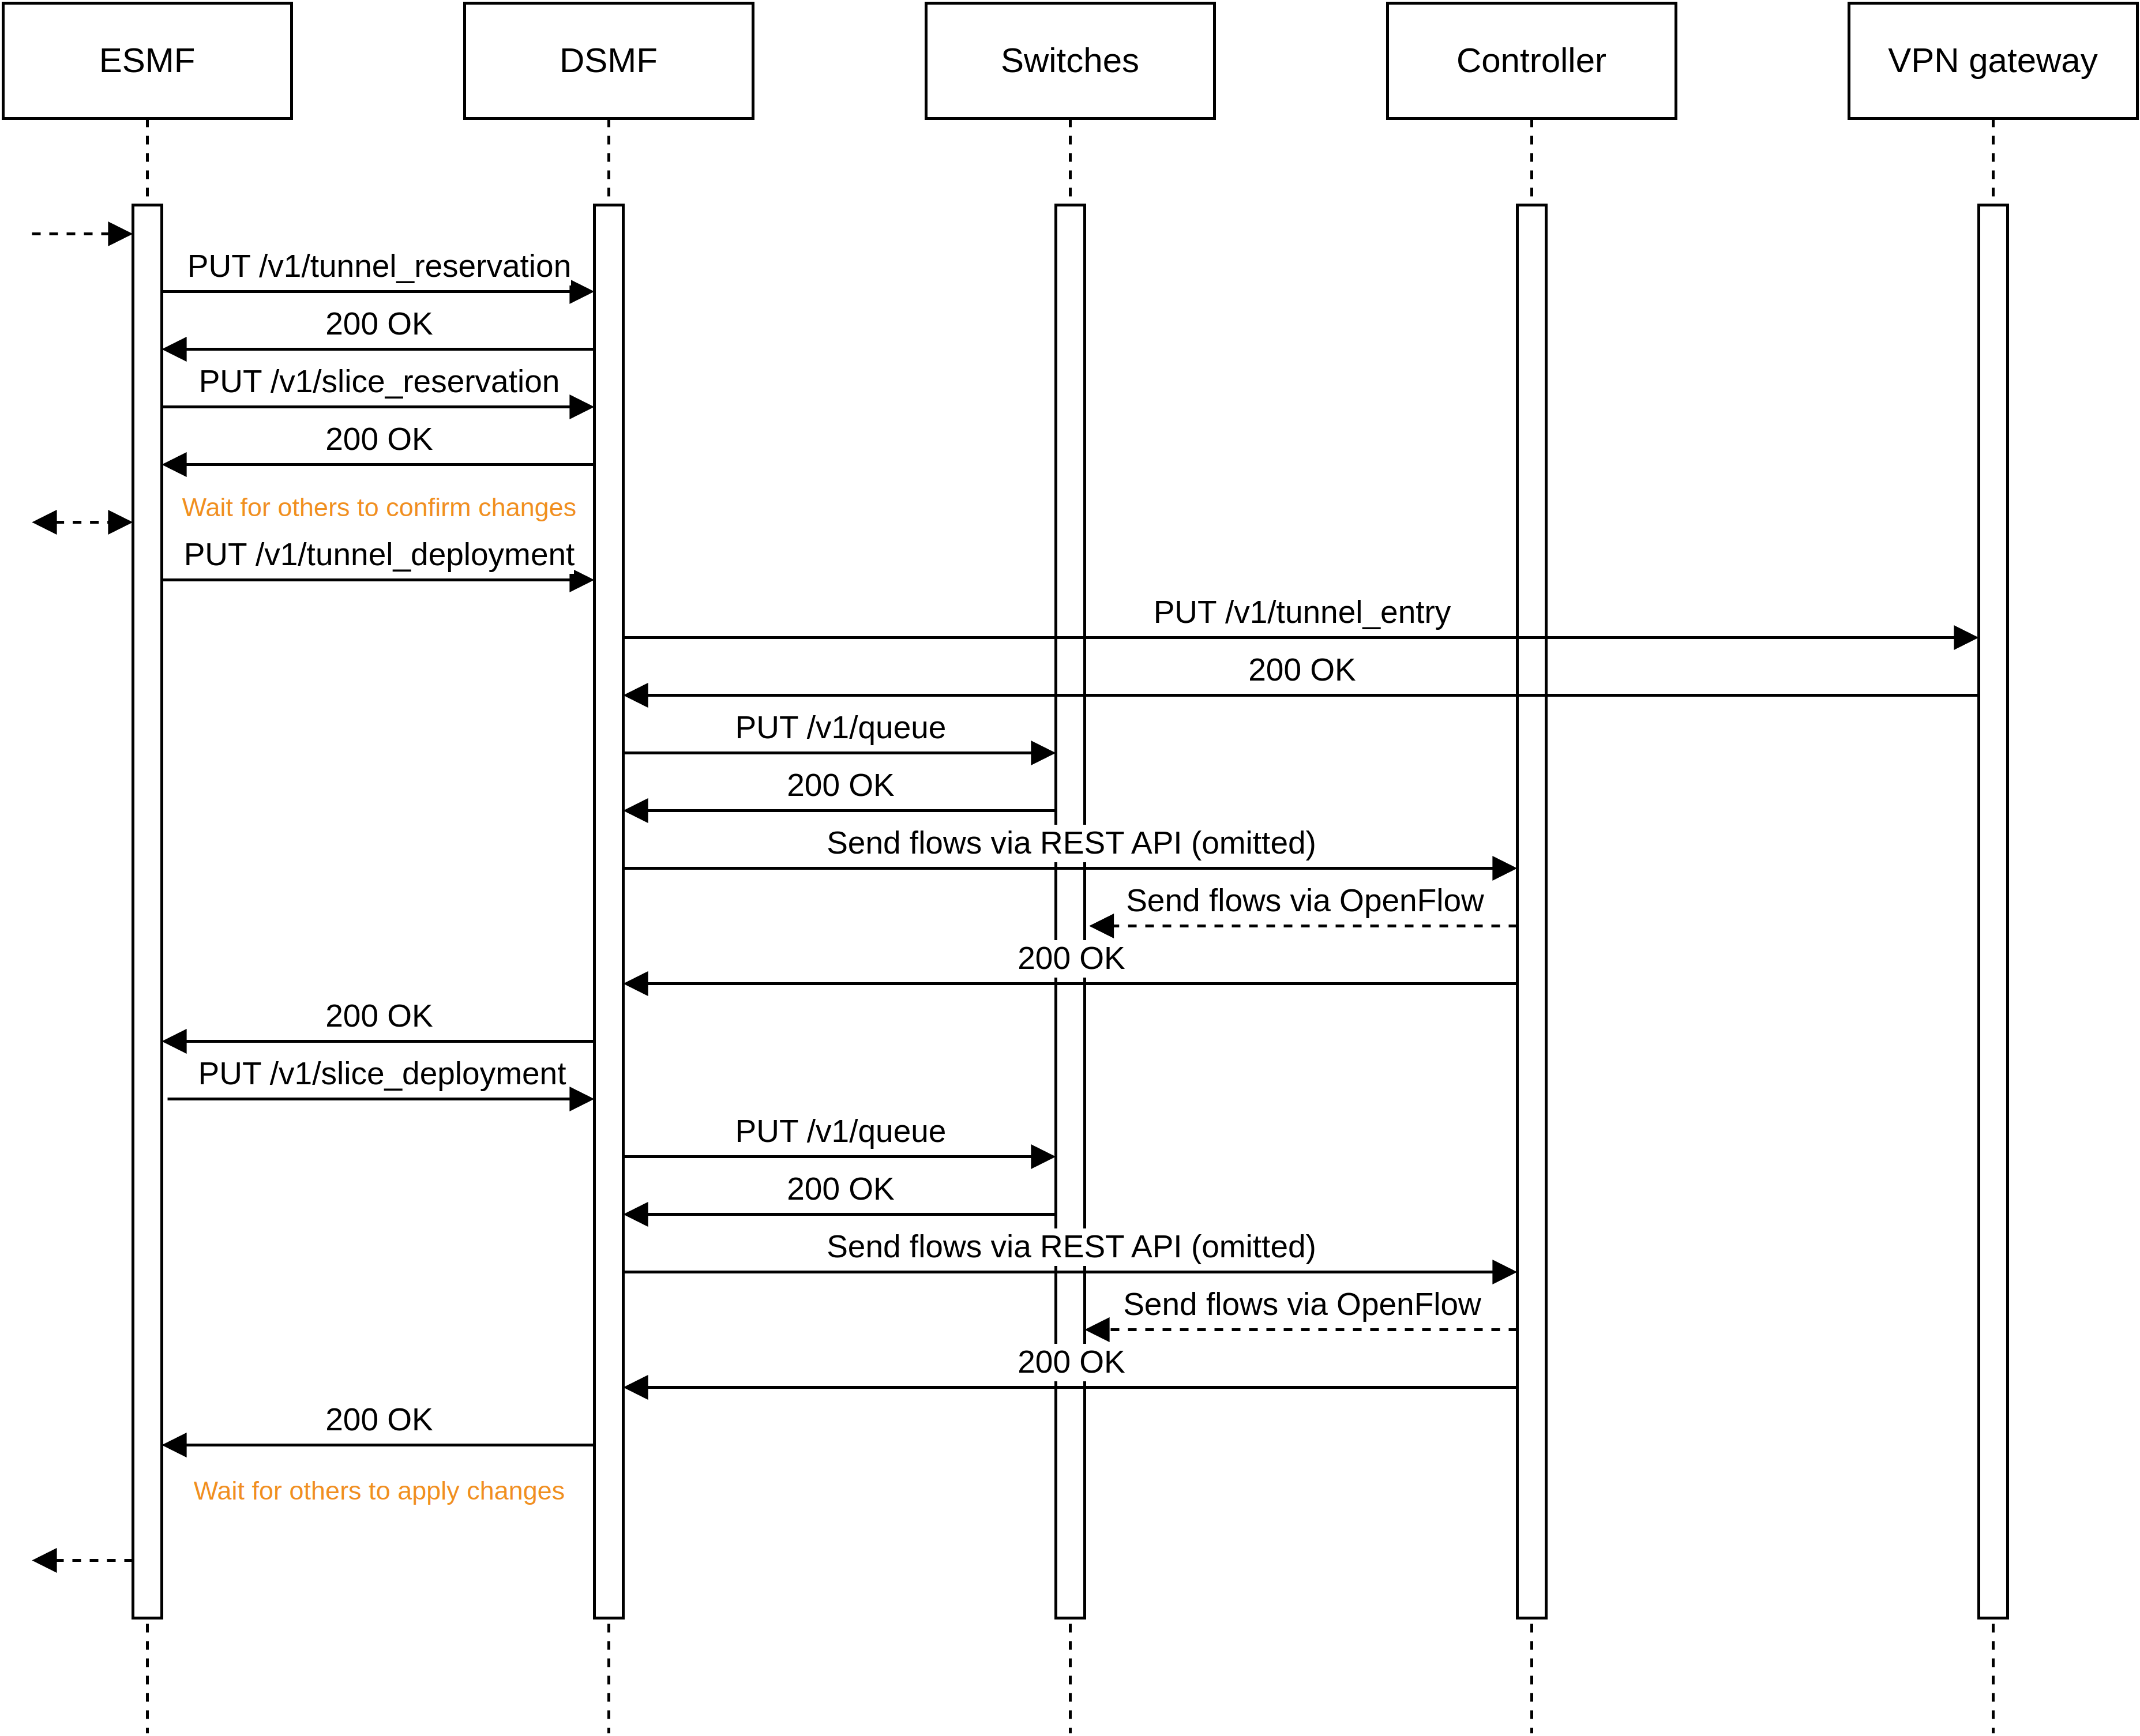
\includegraphics[width=\linewidth]{images/chapter_6/slice_creation_edge.png}
    \caption[Slice creation on an \gls{edgenetwork}]{Communication between \acrshort{esmf}, \acrshort{dsmf}, controller, switches and \acrshort{vpn} gateway on the edge to create a slice illustrated in a sequence diagram. The process seen here deploys the slices and tunnels of a single \gls{edgenetwork}. Requests might be in larger quantity when multiple slices and tunnels get deployed or multiple switches are present. The \acrshort{esmf} will contact the \acrshort{dsmf}, which will then contact the data plane \acrshort{vnf}s to deploy the actual functionality. Everything is guarded by reservations upfront. The dotted arrows to the left indicate synchronization efforts from other \acrshort{esmf}s or communication with the requesting host.}
    \label{fig:slice_creation_edge}
\end{figure}
\begin{figure}[H]
    \centering
    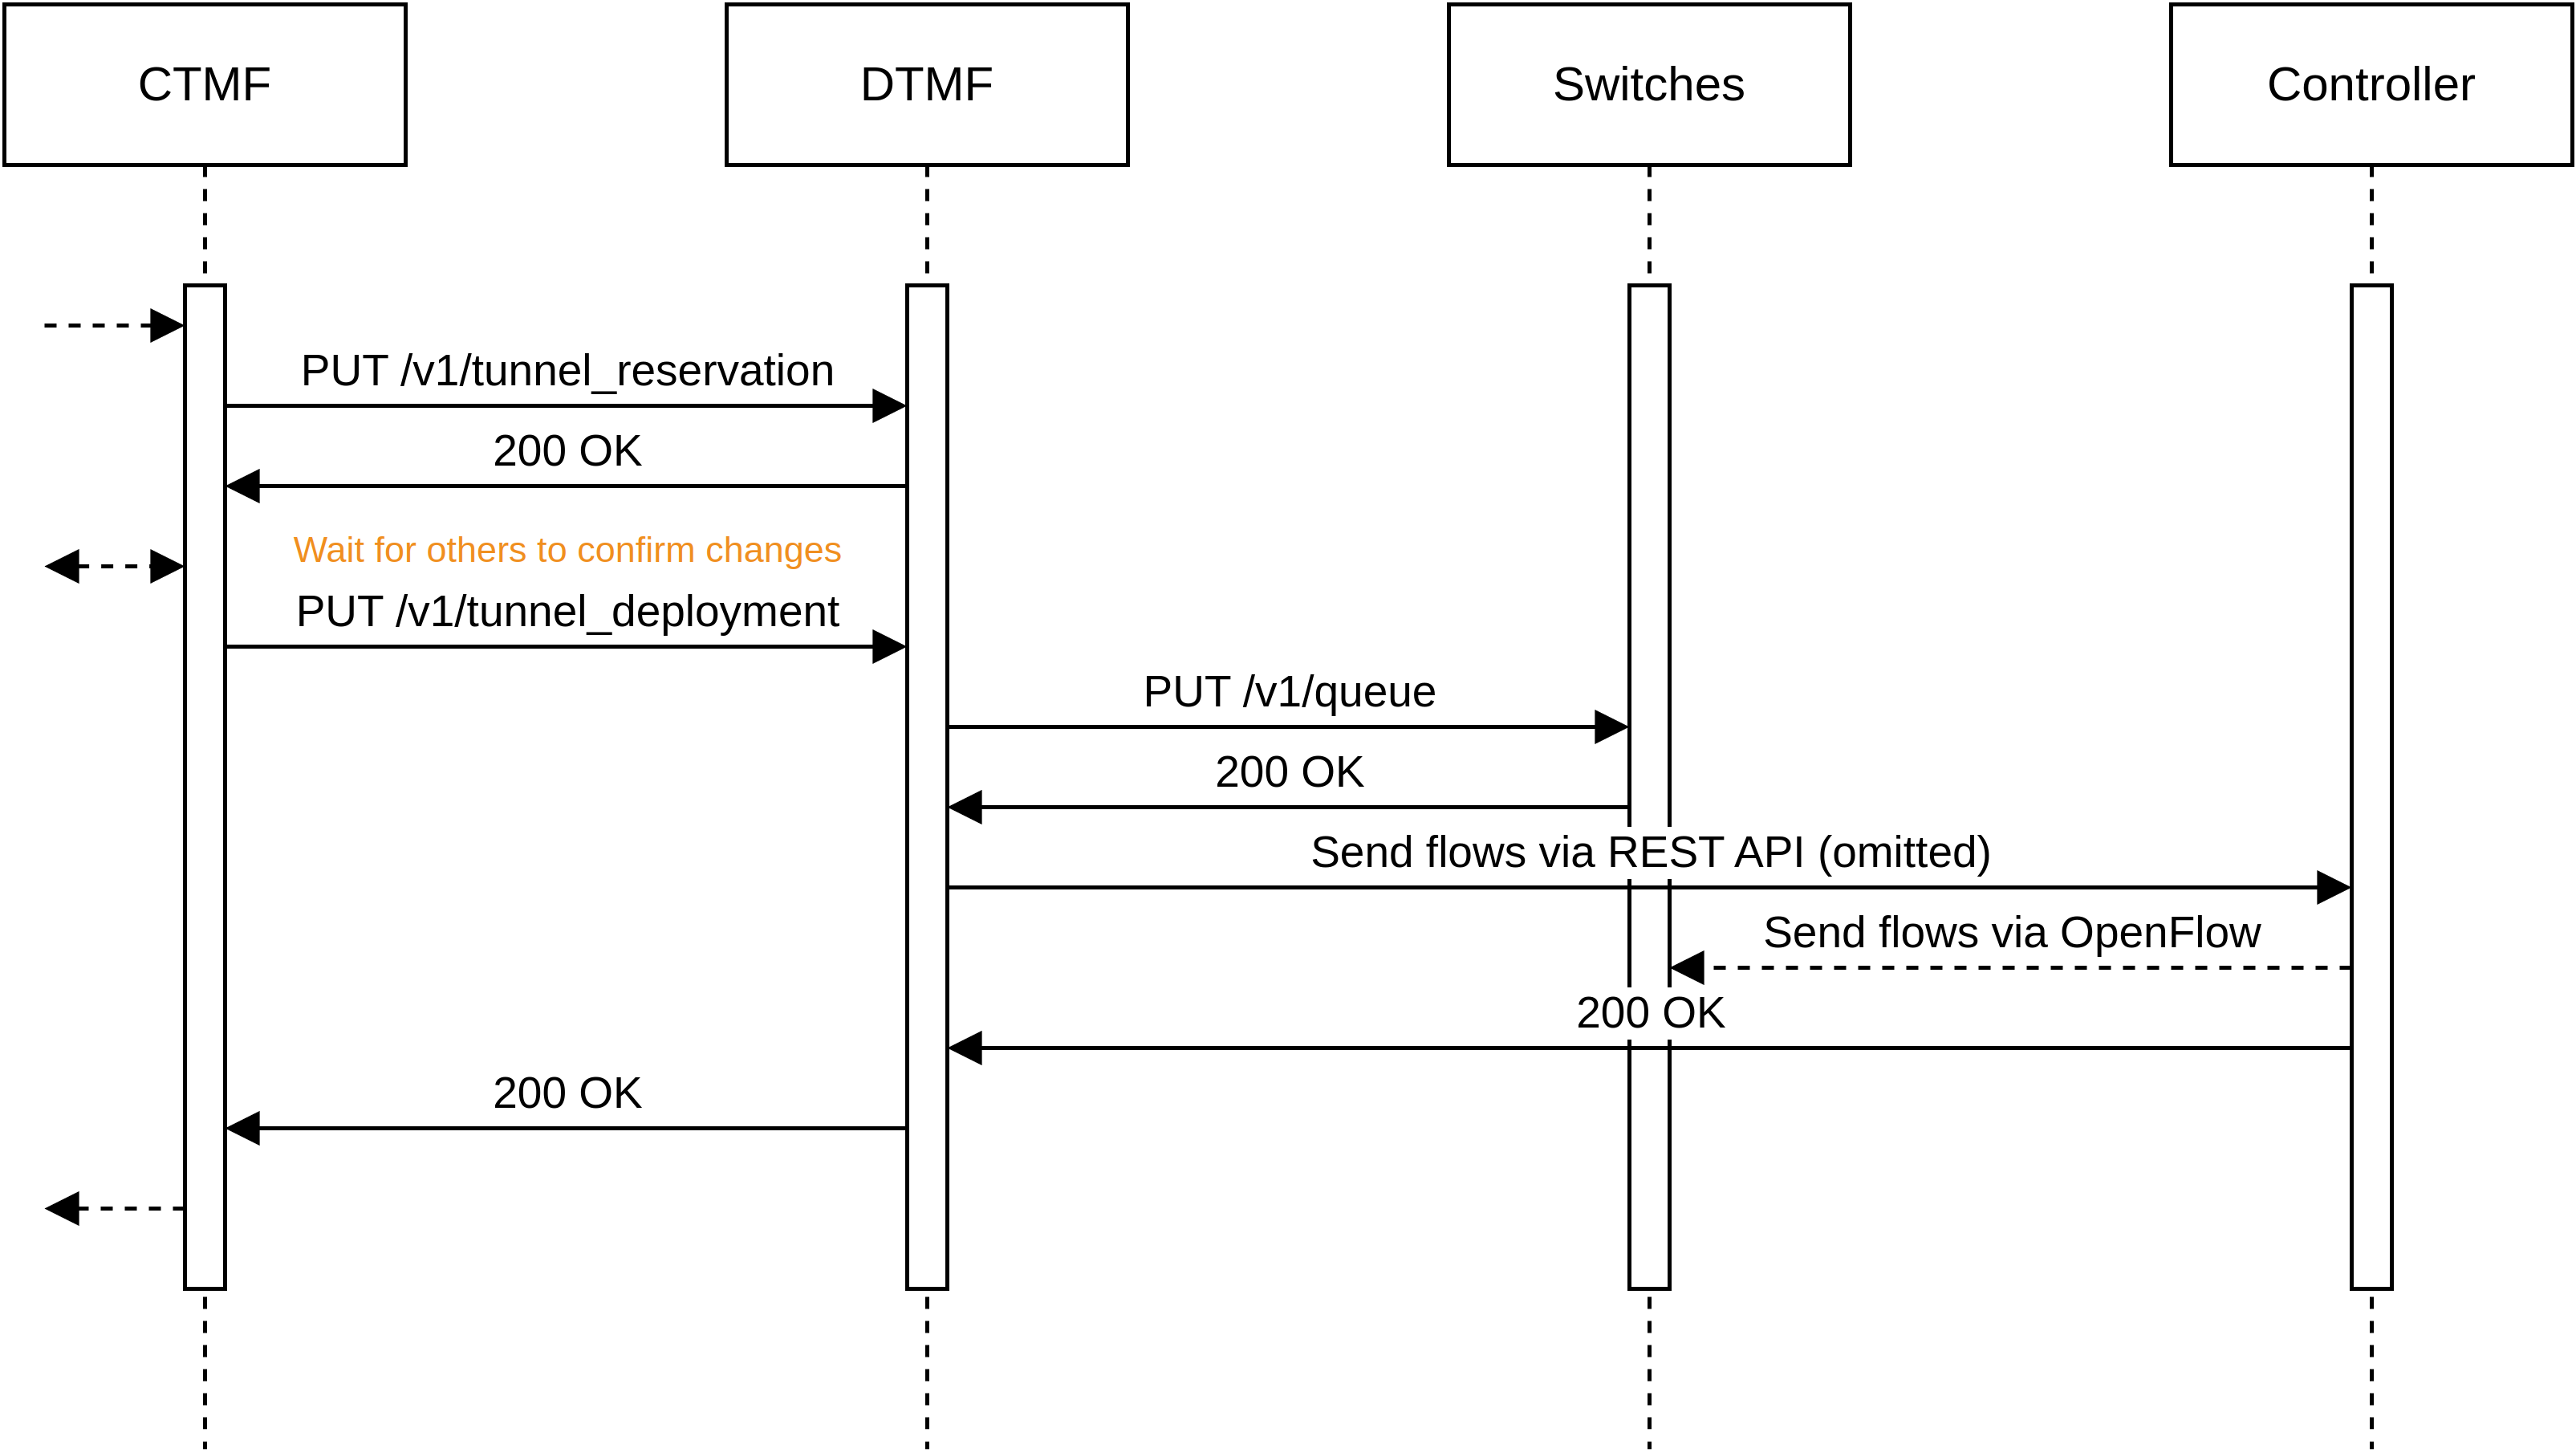
\includegraphics[width=\linewidth]{images/chapter_6/slice_creation_bn.png}
    \caption[Slice creation on a \gls{blacknetwork}]{This figure shows the communication between \acrshort{ctmf}, \acrshort{dtmf}, controller and switches on the \gls{blacknetwork} in a sequence diagram in order to create tunnels. There are no \acrshort{vpn} gateways on \gls{blacknetwork}s, so they do not appear here as compared to the figure on \gls{edgenetwork}s. As previously with \acrshort{esmf} and \acrshort{dsmf}, the \acrshort{ctmf} will contact the \acrshort{dtmf}, which will then instruct the controller and switches to deploy the tunnel functionality. Everything is guarded by reservations upfront. The dotted arrows to the left indicate synchronization efforts from other \acrshort{esmf}s. If there are multiple switches the requests are repeated for each of them.}
    \label{fig:slice_creation_bn}
\end{figure}

\newpage

\subsubsection{Slice removal}
In order to remove a slice the steps mentioned above are basically reversed. In this case we do not use the two-phase commit protocol, as when failing to synchronize the same drawbacks as mentioned above occur, which could be solved by future implementations with ease by removing dangling deployments.

As for the creation of one or multiple slices, the coordinating \acrshort{esmf} is contacted again to remove these slices. The \acrshort{esmf} will create a list of all slices and tunnels affected and issue a removal for them. A tunnel is removed when no slices remain on the tunnel, else the tunnel may be adapted to include less capacity. The \acrshort{esmf} will contact all other participating domain coordinators and state slices and tunnels to be removed. Each domain coordinator, including the coordinating \acrshort{esmf} will then contact the infrastructure coordinator of their domain requesting a removal of all tunnels and slices that are supposed to be removed. The infrastructure providers will then use the before mentioned \acrshort{api}s to remove all components. When everyone reports back a positive result, the host is informed about the positive result of the removal.

As with the previous section, the entire process of removing a slice can also be viewed as sequence diagrams for the state synchronization (see Figure \ref{fig:slice_removal_synchronization}), the communication on the \gls{edgenetwork}s (see Figure \ref{fig:slice_removal_edge}) and on our \gls{blacknetwork}s (see Figure \ref{fig:slice_removal_bn}).

\begin{figure}[H]
    \centering
    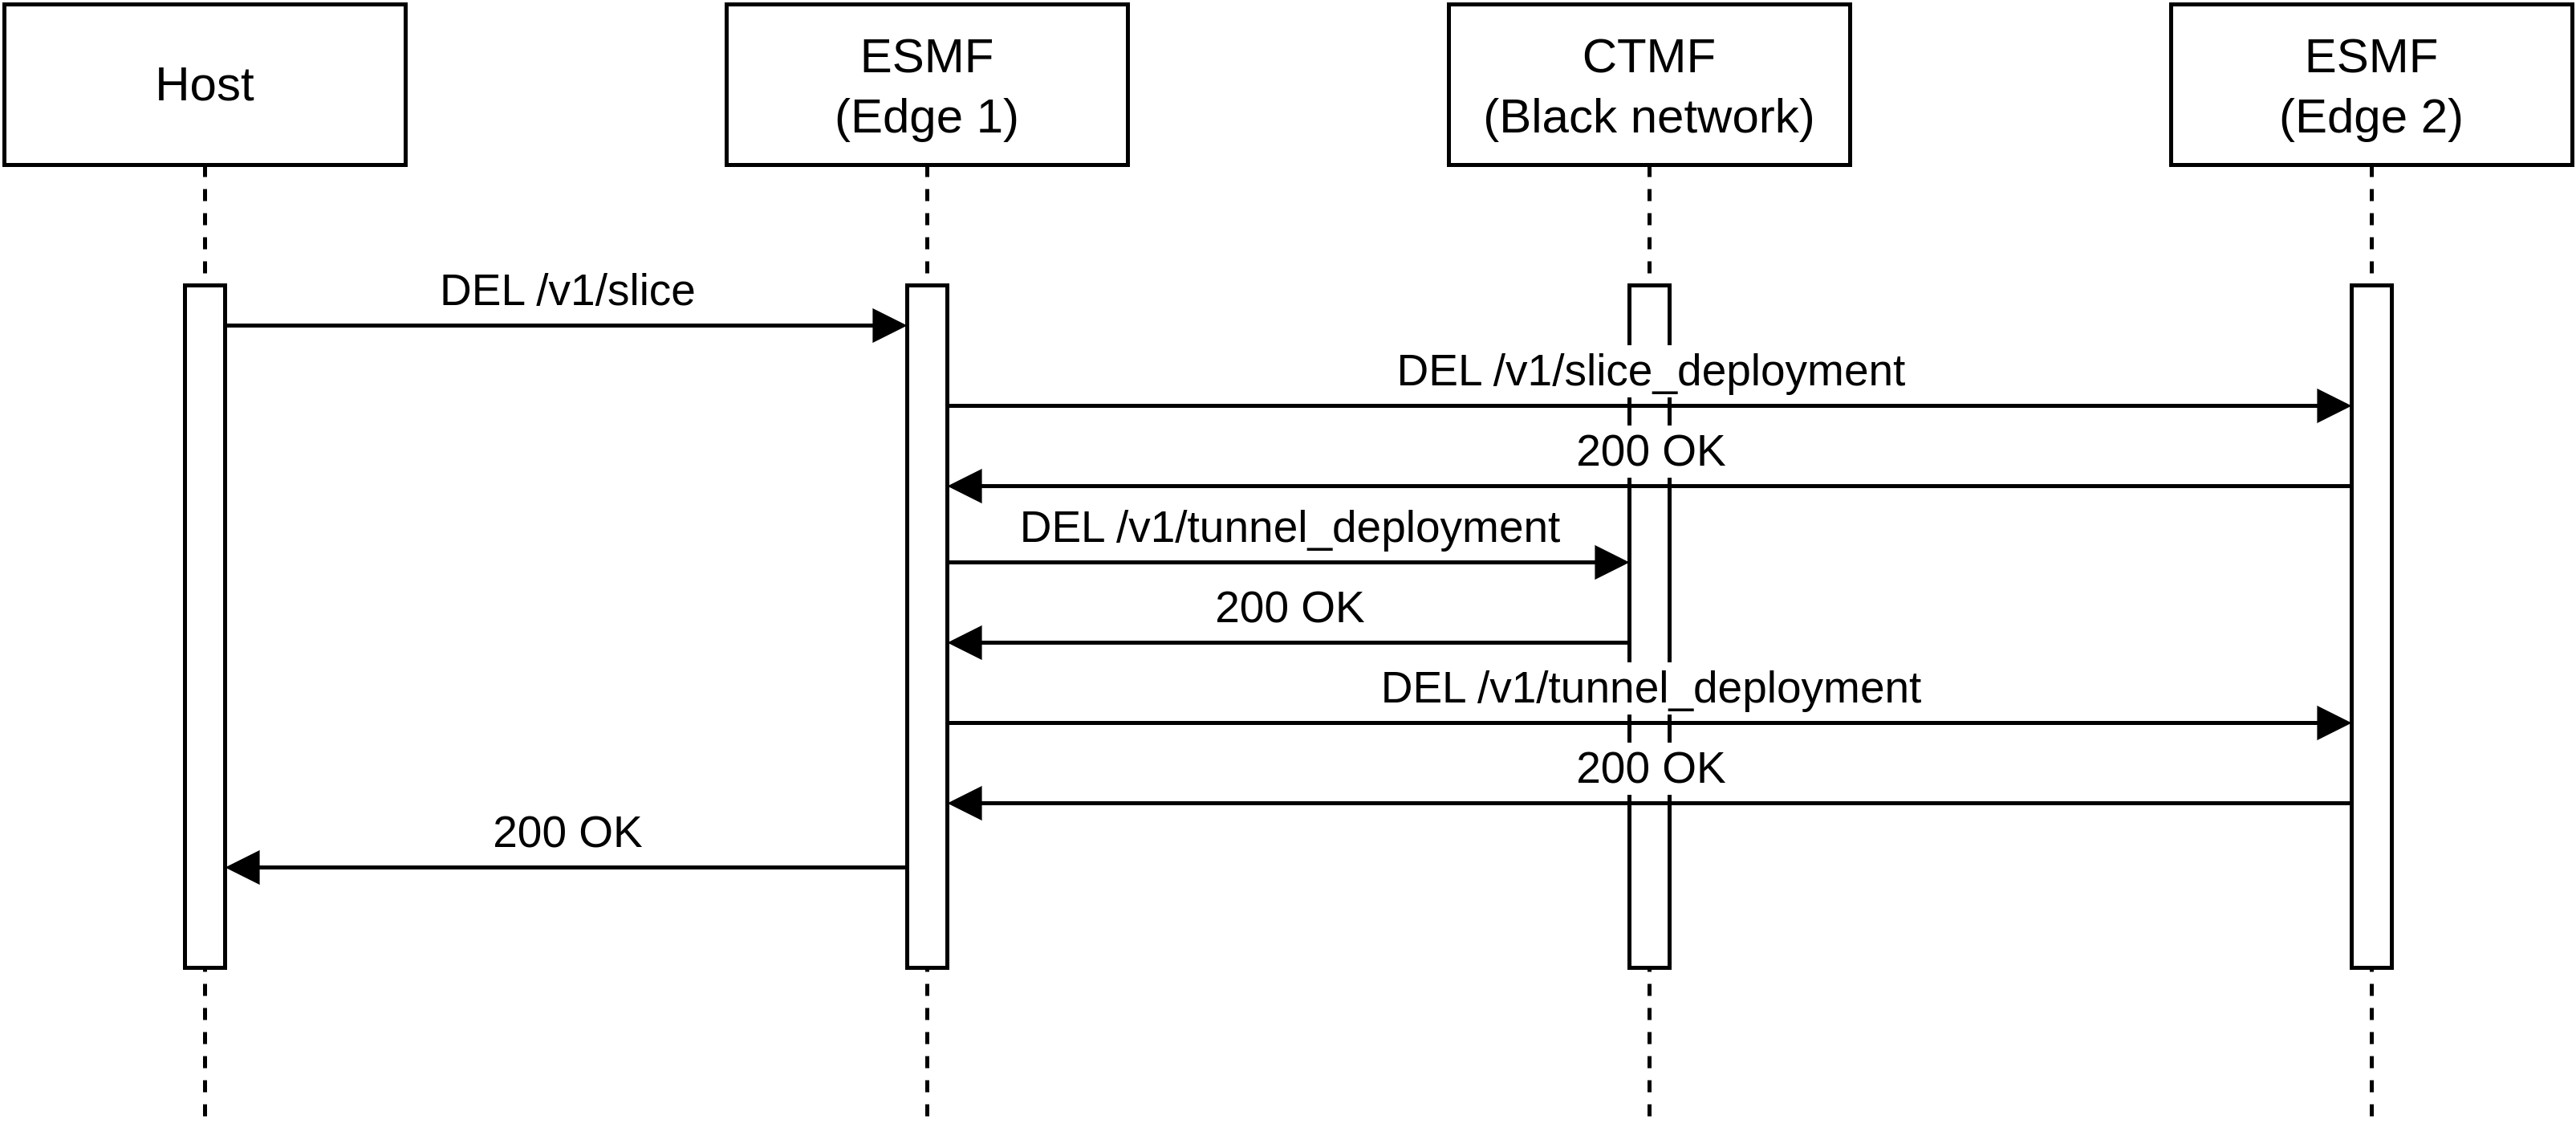
\includegraphics[width=\linewidth]{images/chapter_6/slice_removal_coordination.png}
    \caption[Slice removal on the coordinators]{Removal of slices on the domain coordinator level illustrated in a sequence diagram. The coordinator \acrshort{esmf} that has been contacted by the host will contact all other domain coordinators to remove the slice and all tunnels that have to be removed with the slice or that need to be adapted. Once everyone reports successful removal, the successful result is reported back to the host. If anyone reported a failure to remove, the host will receive a negative reply. If there is more than one \gls{blacknetwork}, the requests for the \acrshort{ctmf} need to be applied on each of them.}
    \label{fig:slice_removal_synchronization}
\end{figure}
\begin{figure}[H]
    \centering
    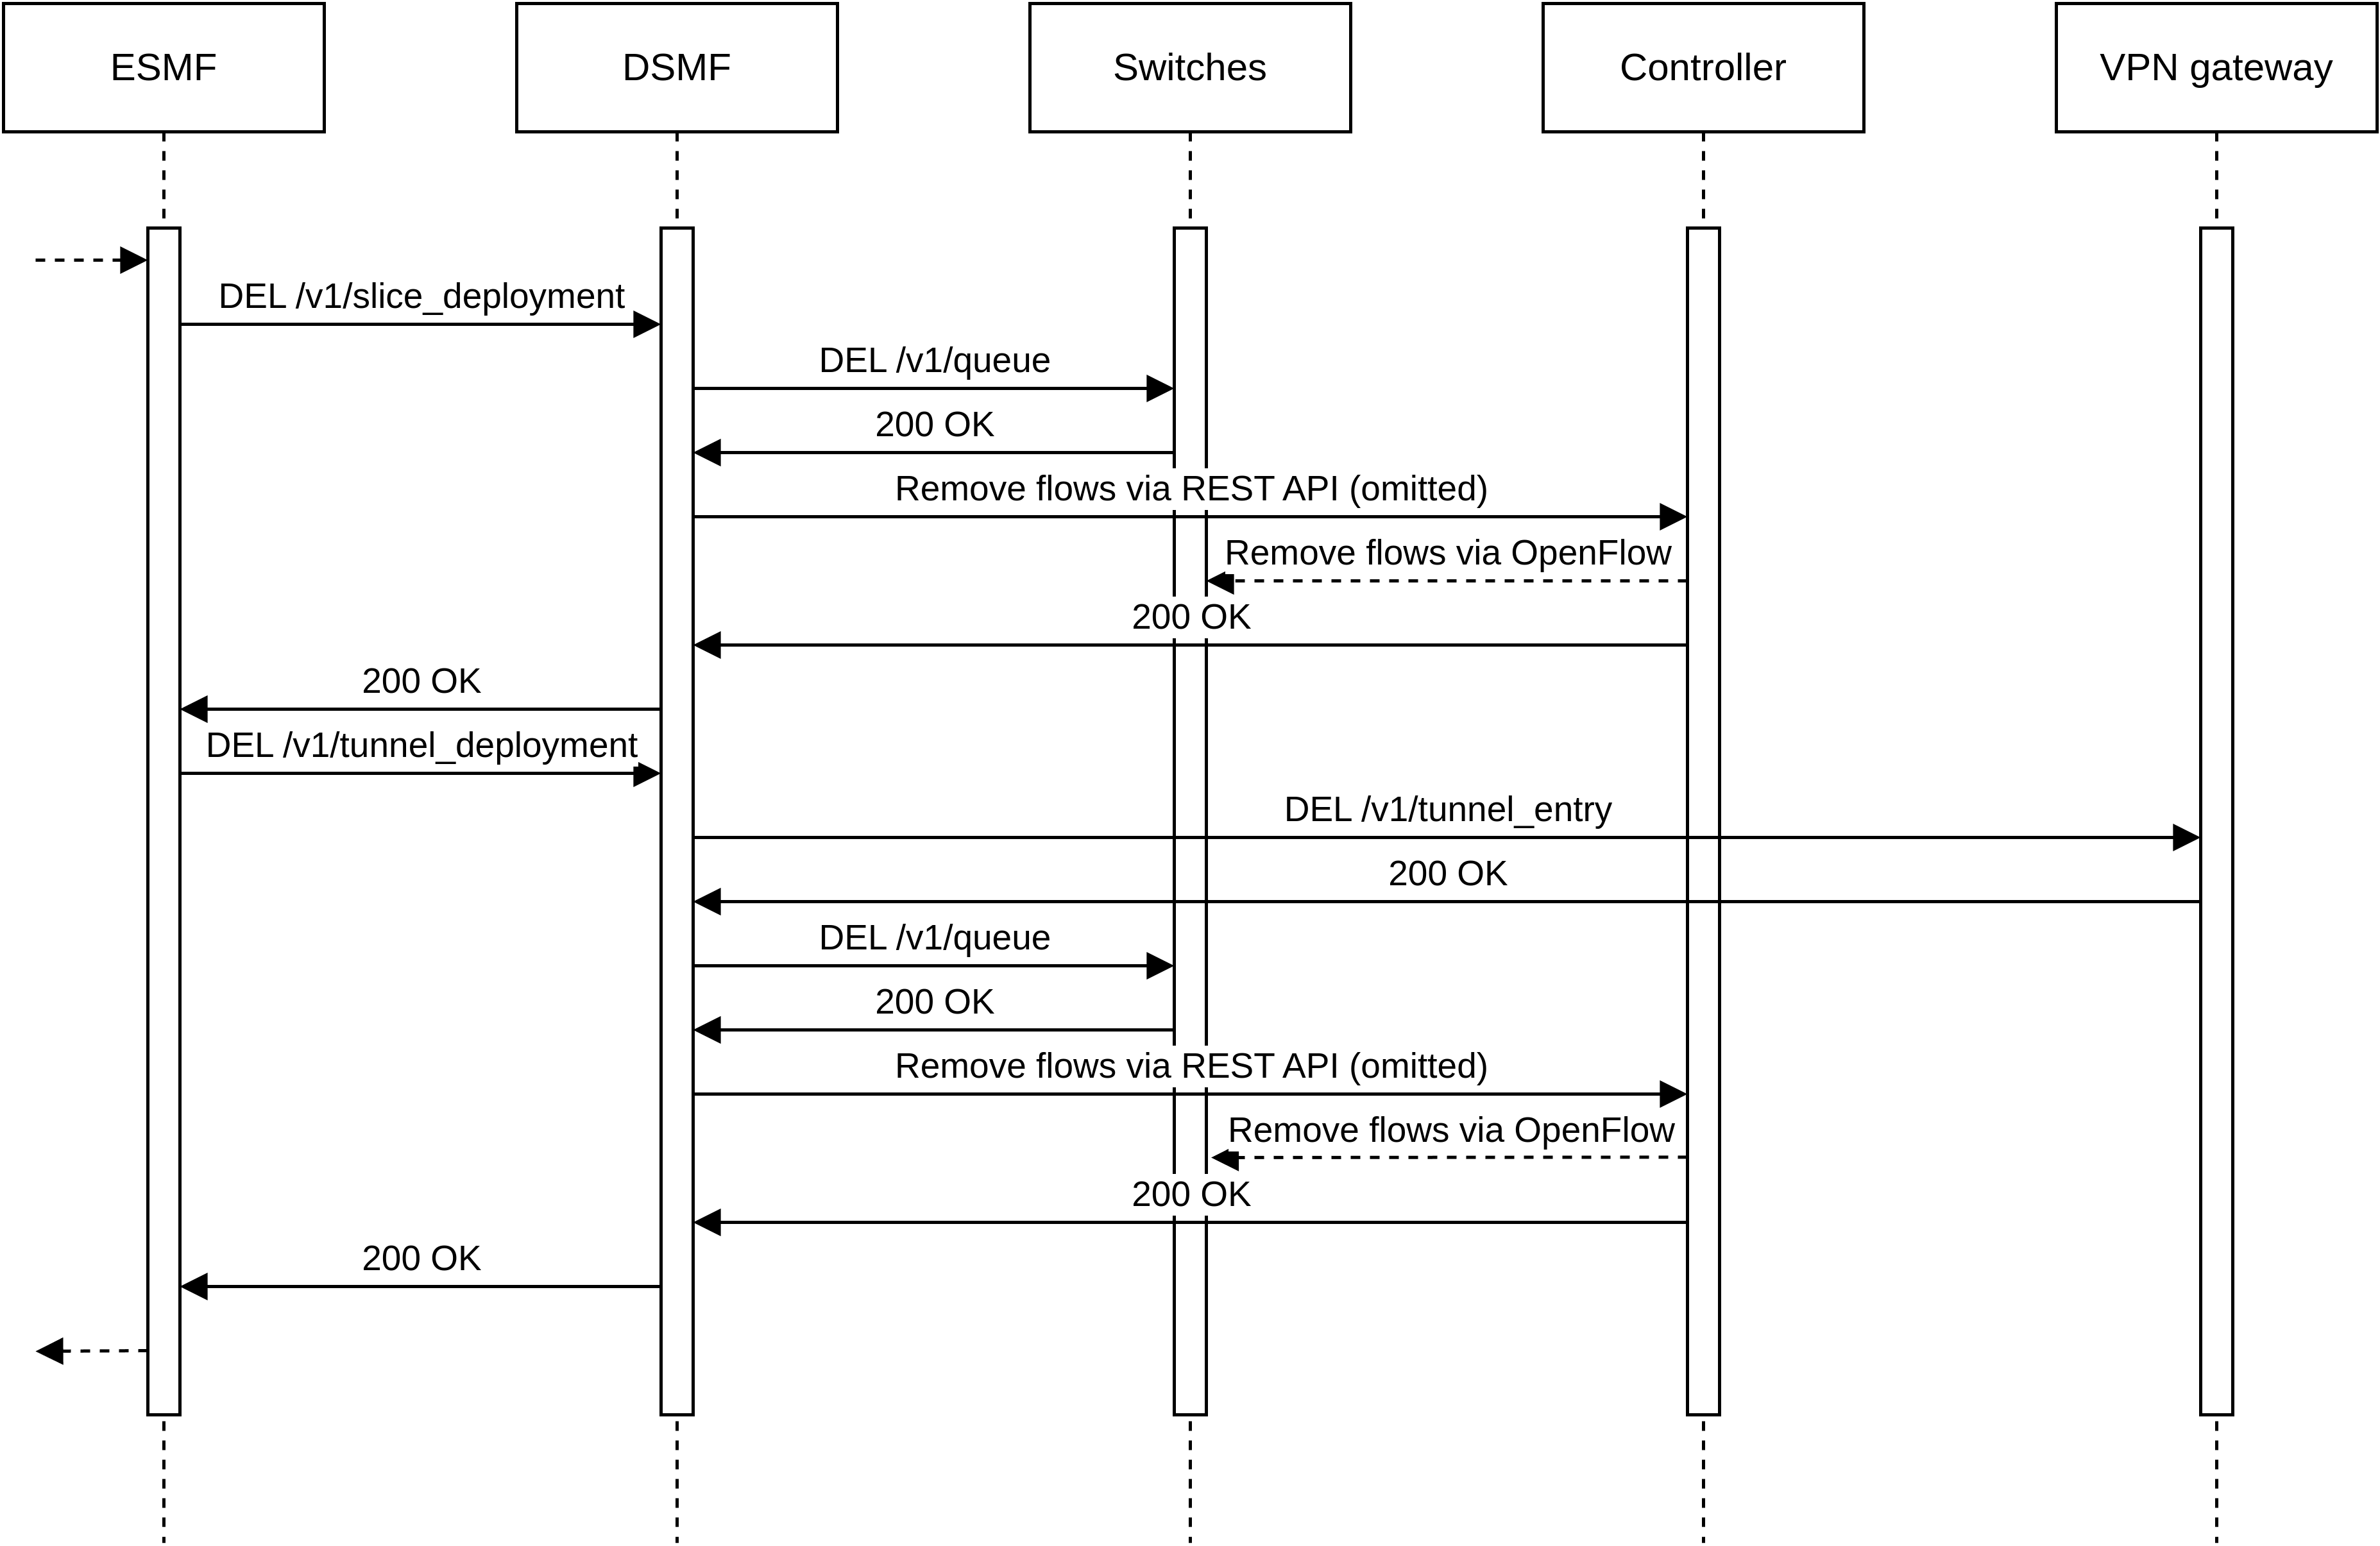
\includegraphics[width=\linewidth]{images/chapter_6/slice_removal_edge.png}
    \caption[Slice removal from an \gls{edgenetwork}]{Sequence diagram showing the removal of slices and tunnels from an \gls{edgenetwork}. The \acrshort{esmf} will contact the \acrshort{dsmf}, which will then instruct controller, switches and \acrshort{vpn} gateway to remove slice and tunnel components. Requests might be in larger quantity when multiple slices and tunnels get removed or multiple switches are present. The dotted arrows to the left indicate synchronization efforts from other \acrshort{esmf}s or communication with the requesting host.}
    \label{fig:slice_removal_edge}
\end{figure}
\begin{figure}[H]
    \centering
    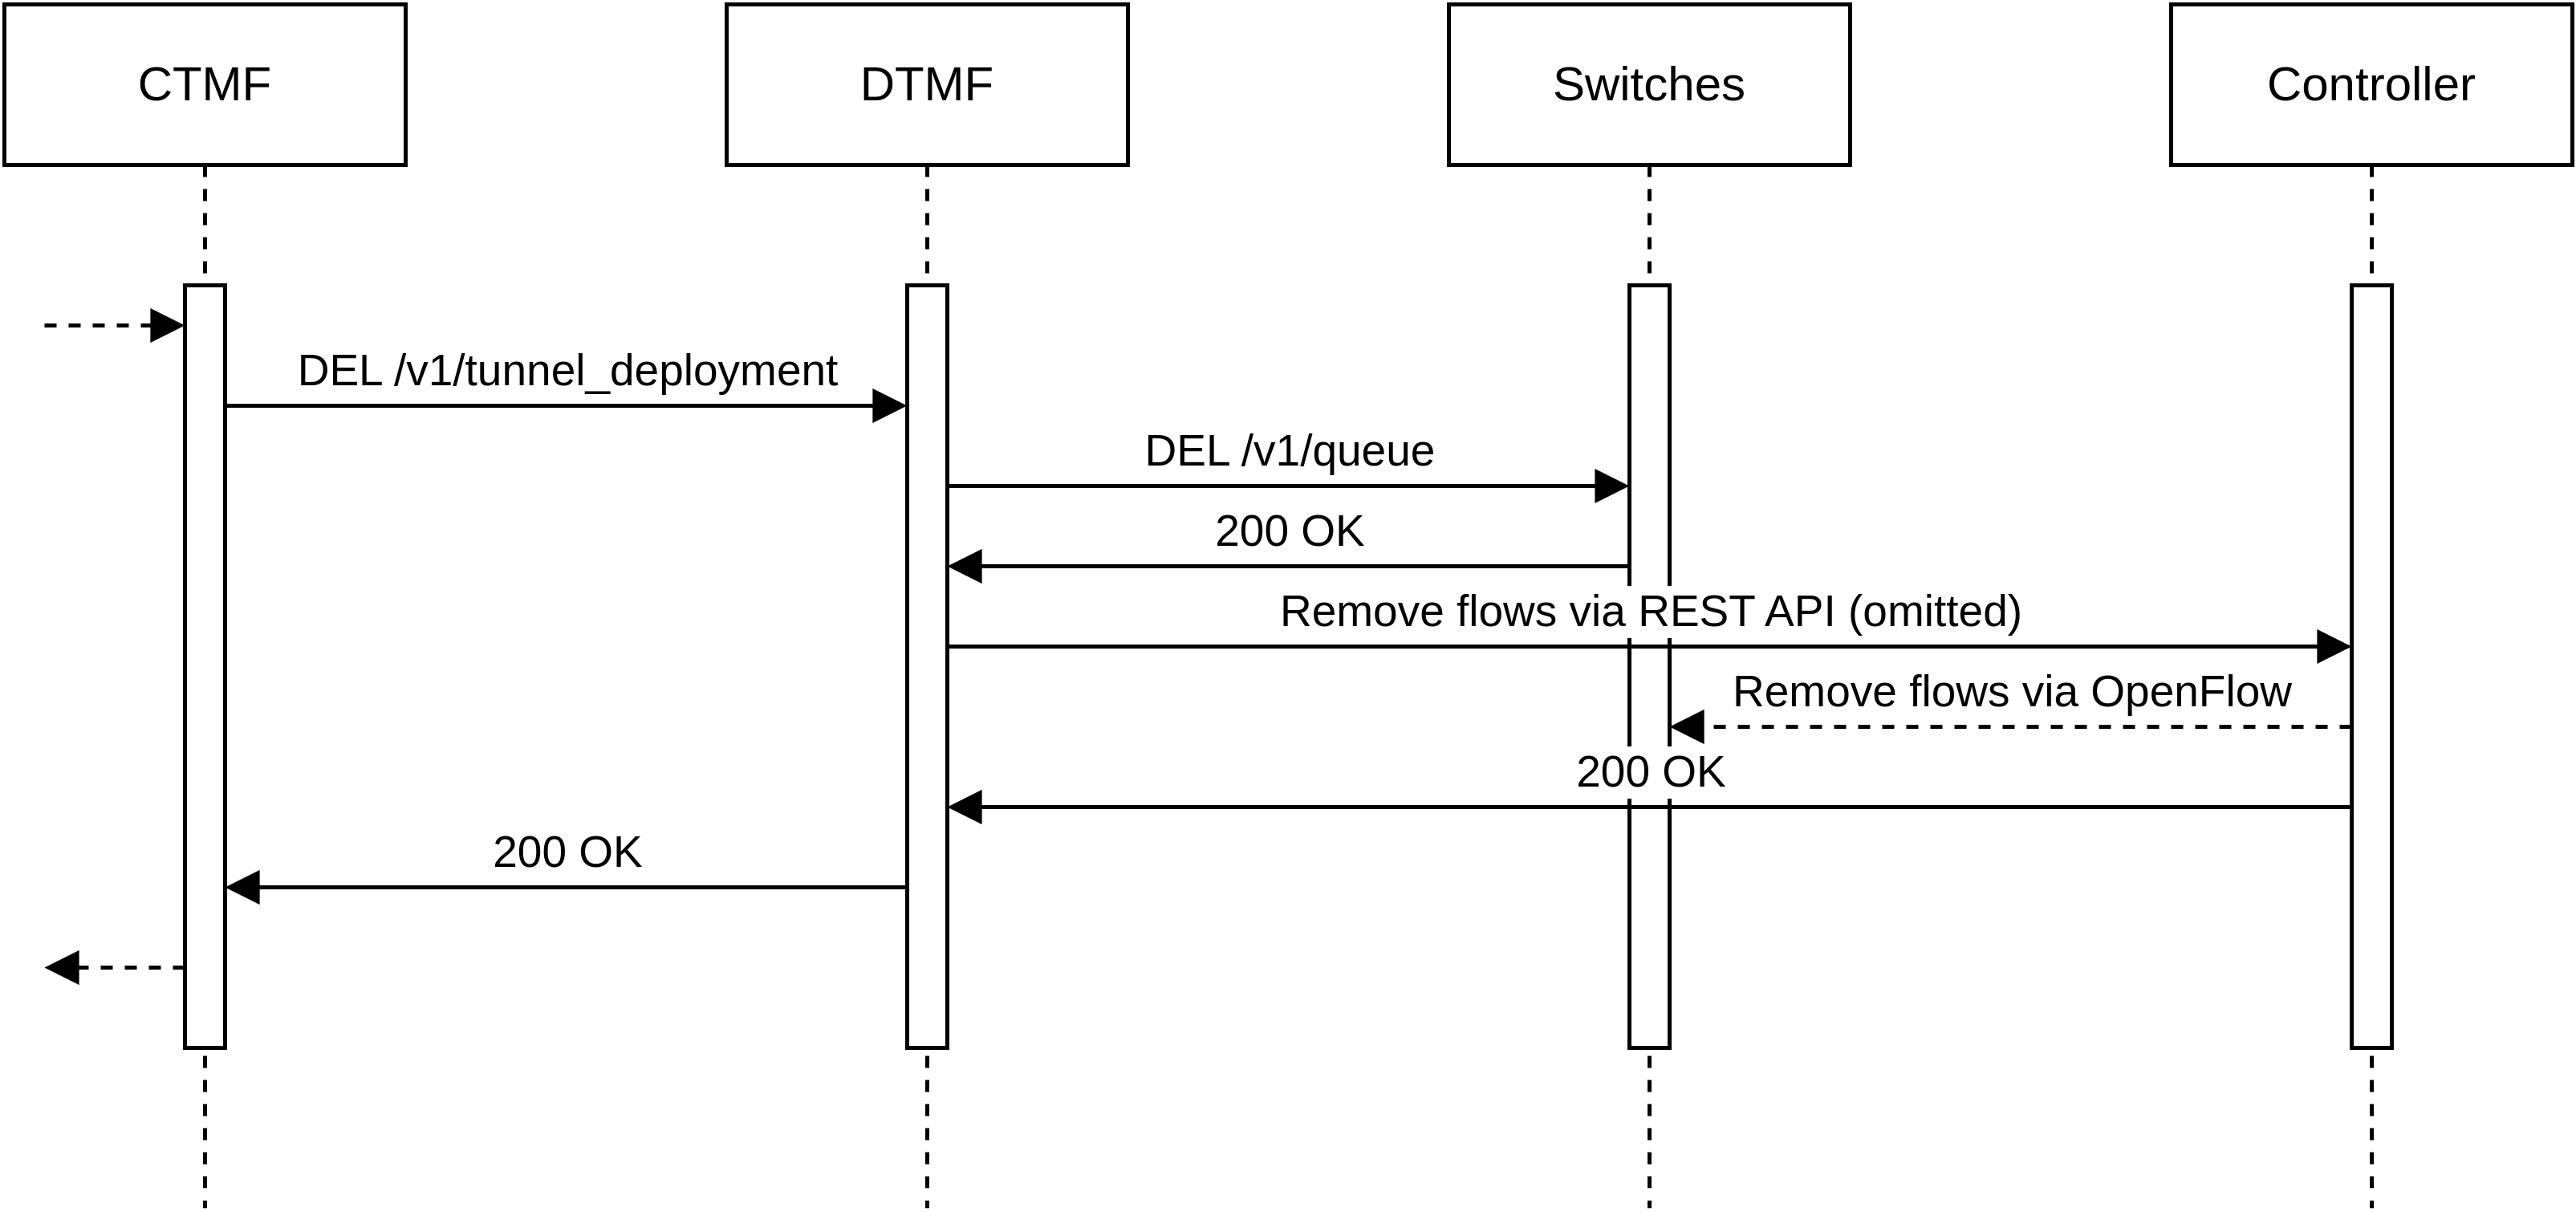
\includegraphics[width=\linewidth]{images/chapter_6/slice_removal_bn.png}
    \caption[Slice removal from a \gls{blacknetwork}]{Sequence diagram showing the removal of tunnels from a \gls{blacknetwork}. The \acrshort{ctmf} will contact the \acrshort{dtmf}, which will then instruct controller and switches to remove the tunnel components. The dotted arrows to the left indicate synchronization efforts from other \acrshort{esmf}s. If there are multiple switches the requests are repeated for each of them.}
    \label{fig:slice_removal_bn}
\end{figure}

\newpage


\section{Components}
In general, all of our \acrshort{vnf}s have been implemented using python. Any version higher than 3.8 should be compatible. The components are shipped as python packages and are pre-installed into \acrshort{lxc} containers (small footprint containers running on the linux platform) \cite{lxc} for use in our validation later. All images come with preinstalled common software and utilities to be able to carry out our validation later and to realize our attackers. Currently included are \textit{iputils-ping} \cite{iputils}, \textit{net-tools} \cite{net-tools}, \textit{iperf3} \cite{iperf3}, \textit{\gls{wireguard}} \cite{wireguard}, \textit{tcpdump} \cite{tcpdump}, \textit{ifstat} (part of \textit{iproute2} \cite{iproute2}), \textit{hping3} \cite{hping3} and \textit{sockperf} \cite{sockperf}. If a package is missing on certain components, it can be integrated by adapting the setup instructions if required.

Some images have additional software apart from above. These and their functionality are stated here:

\paragraph{Application plane components} All components on the application plane (\acrshort{esmf}, \acrshort{ctmf}, \acrshort{dsmf}, \acrshort{dtmf}) have their designated server implementation running, performing their coordination and management duties described in Section \ref{impl_specification}.

\paragraph{Switches} The switches currently use \Gls{ovs} (OVS) \cite{openvswitch} to deploy \acrshort{sdn} switch functionality. Additionally a switch server implementation is executed which issues commands to manage queues and ingress policies on switch ports.

\paragraph{Controller} The controller is realized by utilizing the \Gls{ryu} \cite{ryu} with the common RYU \acrshort{rest} \acrshort{api} \cite{ryu-rest}.

\paragraph{\acrshort{vpn} gateways} The \acrshort{vpn} gateways run a server implementation that allows the creation of \gls{wireguard} \cite{wireguard} tunnel entries. The details of these tunnel entries are explained below in Section \ref{impl_concepts}.


\section{Concepts and configuration}
\label{impl_concepts}
Now that we have established how we wish to deploy tunnels and slices, we still need to specify how the exact configuration on the hardware should be performed.

For simplicity of our implementation, we do not deploy bi-directional slices or tunnels, but rather deploy two uni-directional slices or tunnels to build one single bi-directional one.

A summary of all the flow rules can be seen in figures \ref{fig:routing_source}, \ref{fig:routing_destination} and \ref{fig:routing_bn}.

\subsection{General switch configuration}
To configure a switch we first specify ingress limits on all interfaces, setting the maximum allowed rate and burst to 1Gbit/s. This can of course be adapted for other use cases in the future. This is realised by OVS using a token bucket filter. This way the maximum needed computational capacity of our switch can be evaluated better and an upper limit is provided.

\subsection{Slice configuration}
Slices are configured by deploying flows to our slice switches. For this, we install queues to be used by our flows on each switch participating in the slice first that will then be used by our slice flows. To begin creating the flows the switches are first assigned roles.

We first configure the switches between the origin of our slice and the \acrshort{vpn} gateway. We currently always expect that the slice uses a tunnel and therefore has a \acrshort{vpn} gateway it needs to enter.

If there is only one switch, the switch takes the \textit{SRC\_ALL} role, because it contains all functionality of the source network. If there are multiple switches, the first switch will take the \textit{SRC\_ENTRY} role and the last switch the \textit{SRC\_EXIT} role. All switches between will be assigned a \textit{SRC\_TP} role, indicating that they are transport switches on the source network.

\begin{figure}[ht]
    \centering
    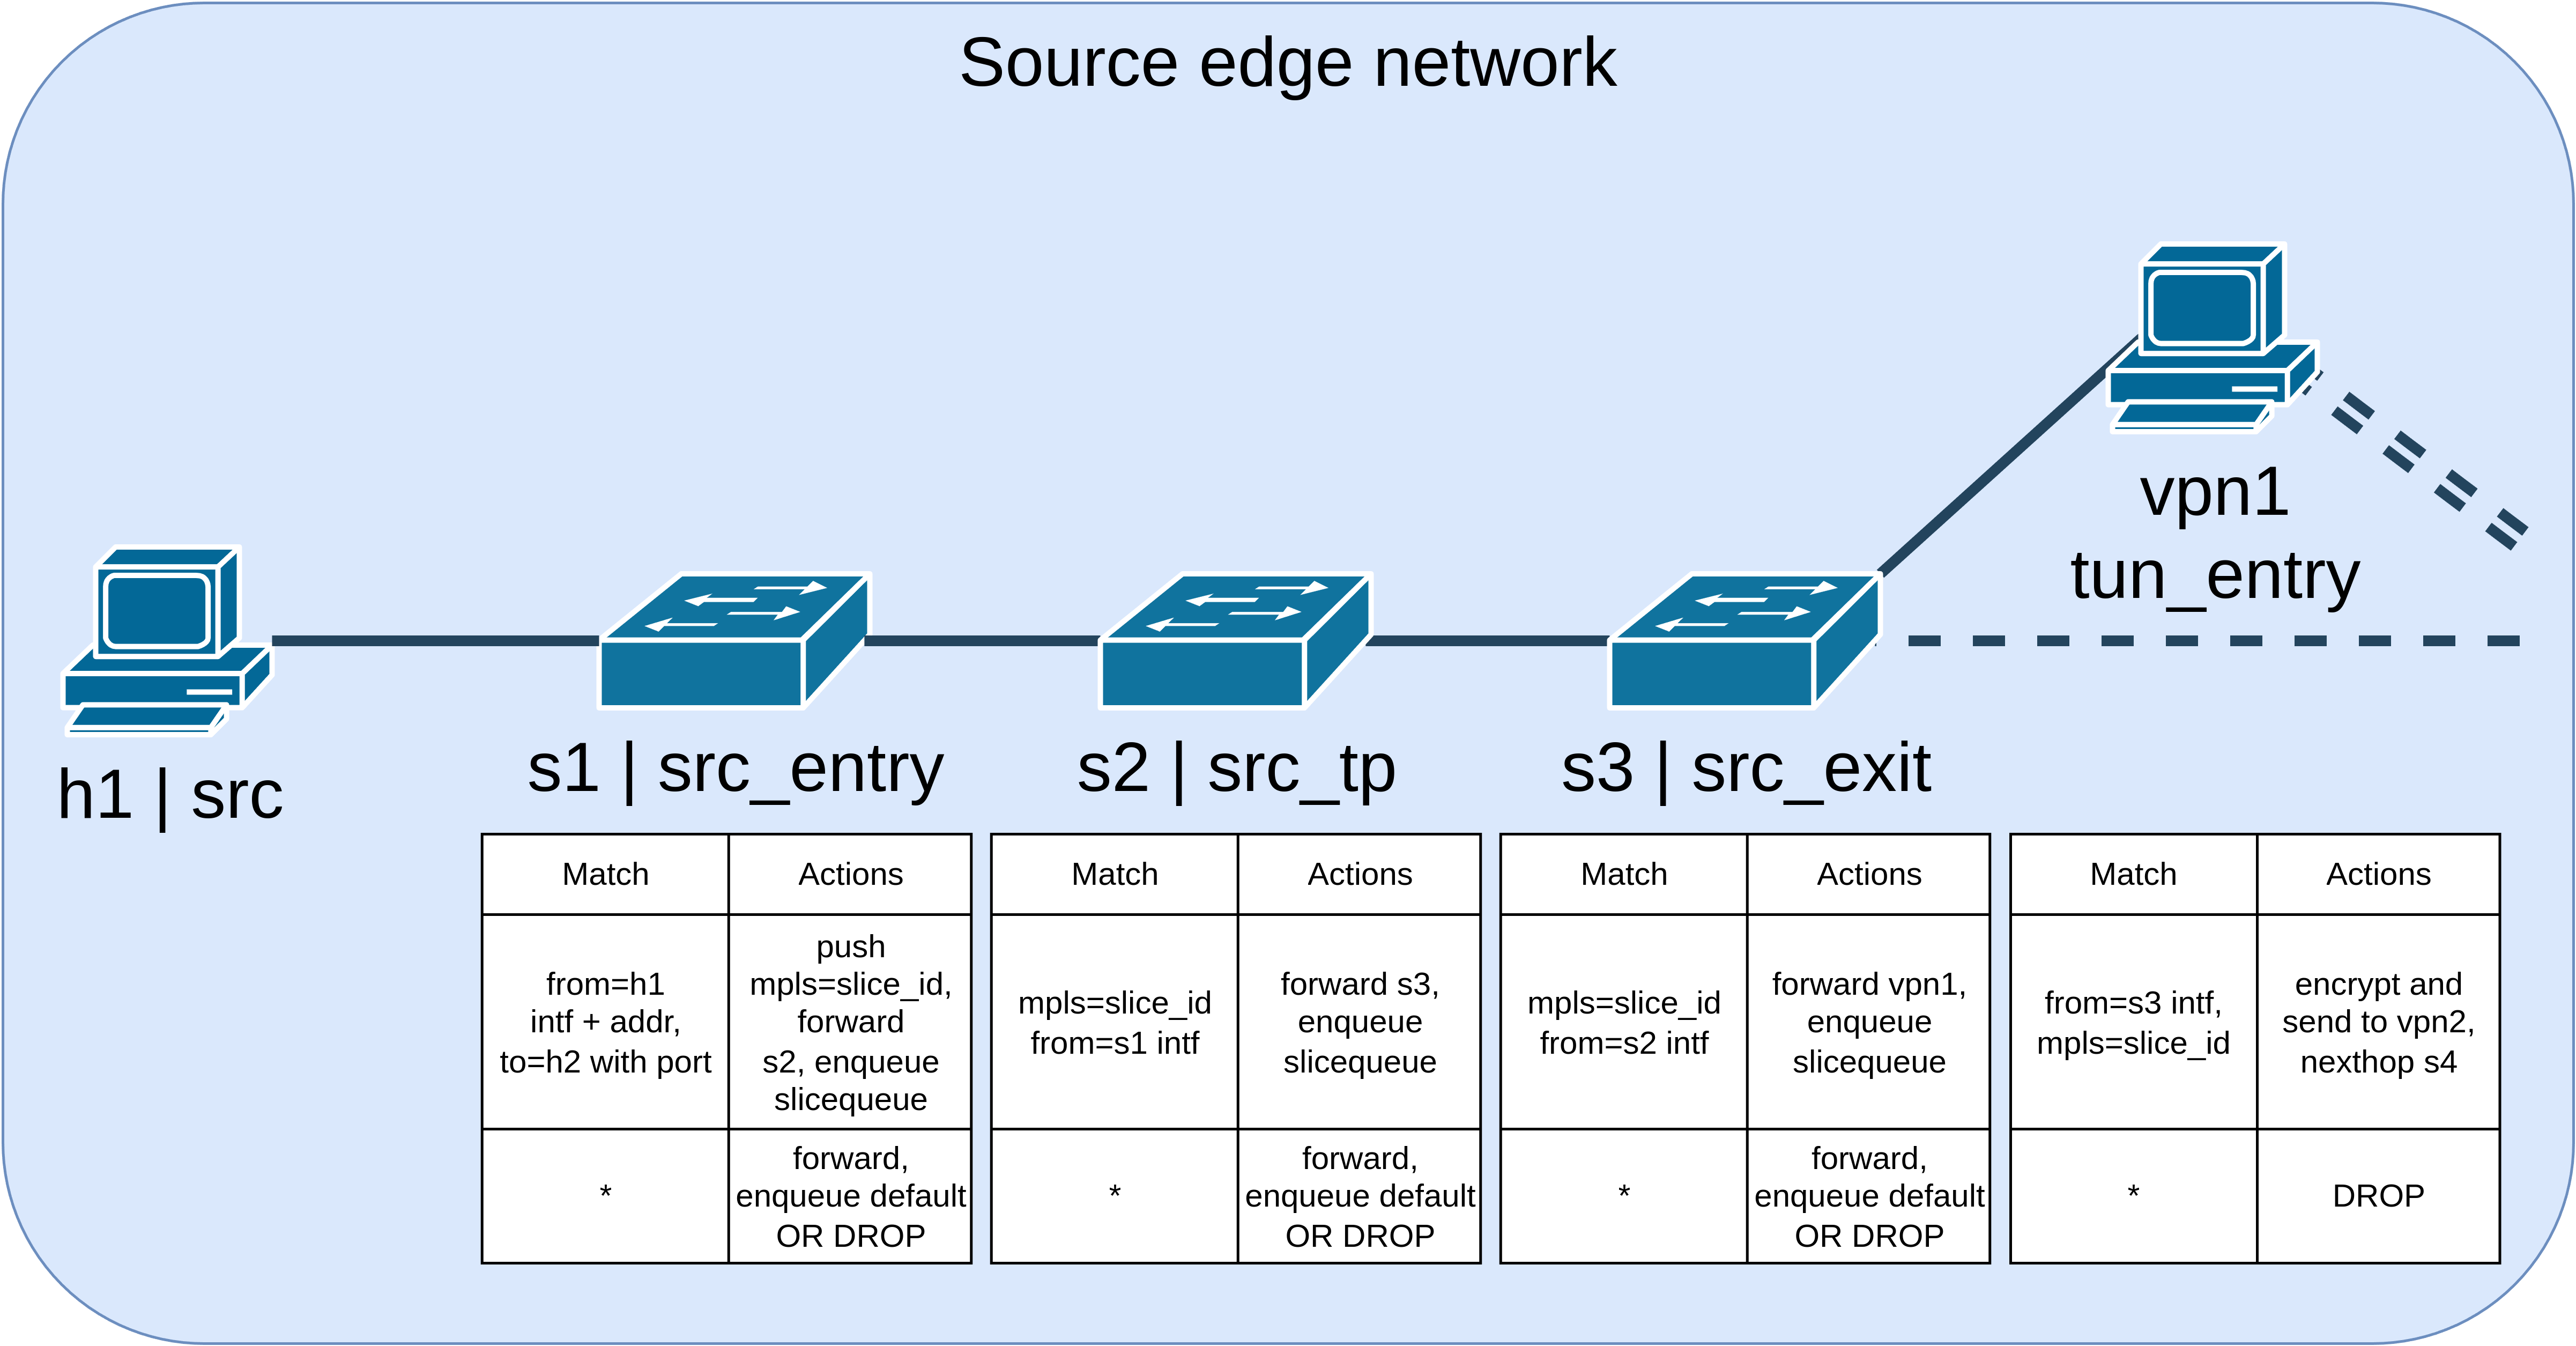
\includegraphics[width=10cm]{images/chapter_6/routing_source.png}
    \caption[Routing on the source \gls{edgenetwork}]{The routing rules on the source \gls{edgenetwork} for the switches and \acrshort{vpn} gateways according to their roles. The dotted lines lead to the first \gls{blacknetwork} switch.}
    \label{fig:routing_source}
\end{figure}

Depending on the role we then deploy the following rules (see Figure \ref{fig:routing_source}):

\paragraph{SRC\_ALL and SRC\_ENTRY} Will verify that a packet matches a slice including the transport destination and port, as well as the incoming interface for authentication purposes. The switch will then tag the packet with an \acrshort{mpls} label using the slice ID as value. The packet will then be forwarded to the next hop.

\paragraph{SRC\_TP and SRC\_EXIT} Will verify that a packet matches a slice by inspecting the slice ID \acrshort{mpls} label and the inbound interface. Will then forward the packet to the next hop. This way, when the next hop is a \acrshort{vpn} gateway, the \acrshort{vpn} gateway will send the slice ID through the tunnel as well.

\paragraph{} Similar to the source network, on the destination network the route from the \acrshort{vpn} gateway to the destination host will be determined and the switches will be assigned roles. These switches will receive the same roles as on the source network, but will be prefixed with \textit{DST} instead. We thus have \textit{DST\_ENTRY} for the switch after the \acrshort{vpn} gateway, then possibly multiple \textit{DST\_TP} switches, before reaching the \textit{DST\_EXIT} switch. As previously, these roles can be combined to form a \textit{DST\_ALL} switch.

\begin{figure}[ht]
    \centering
    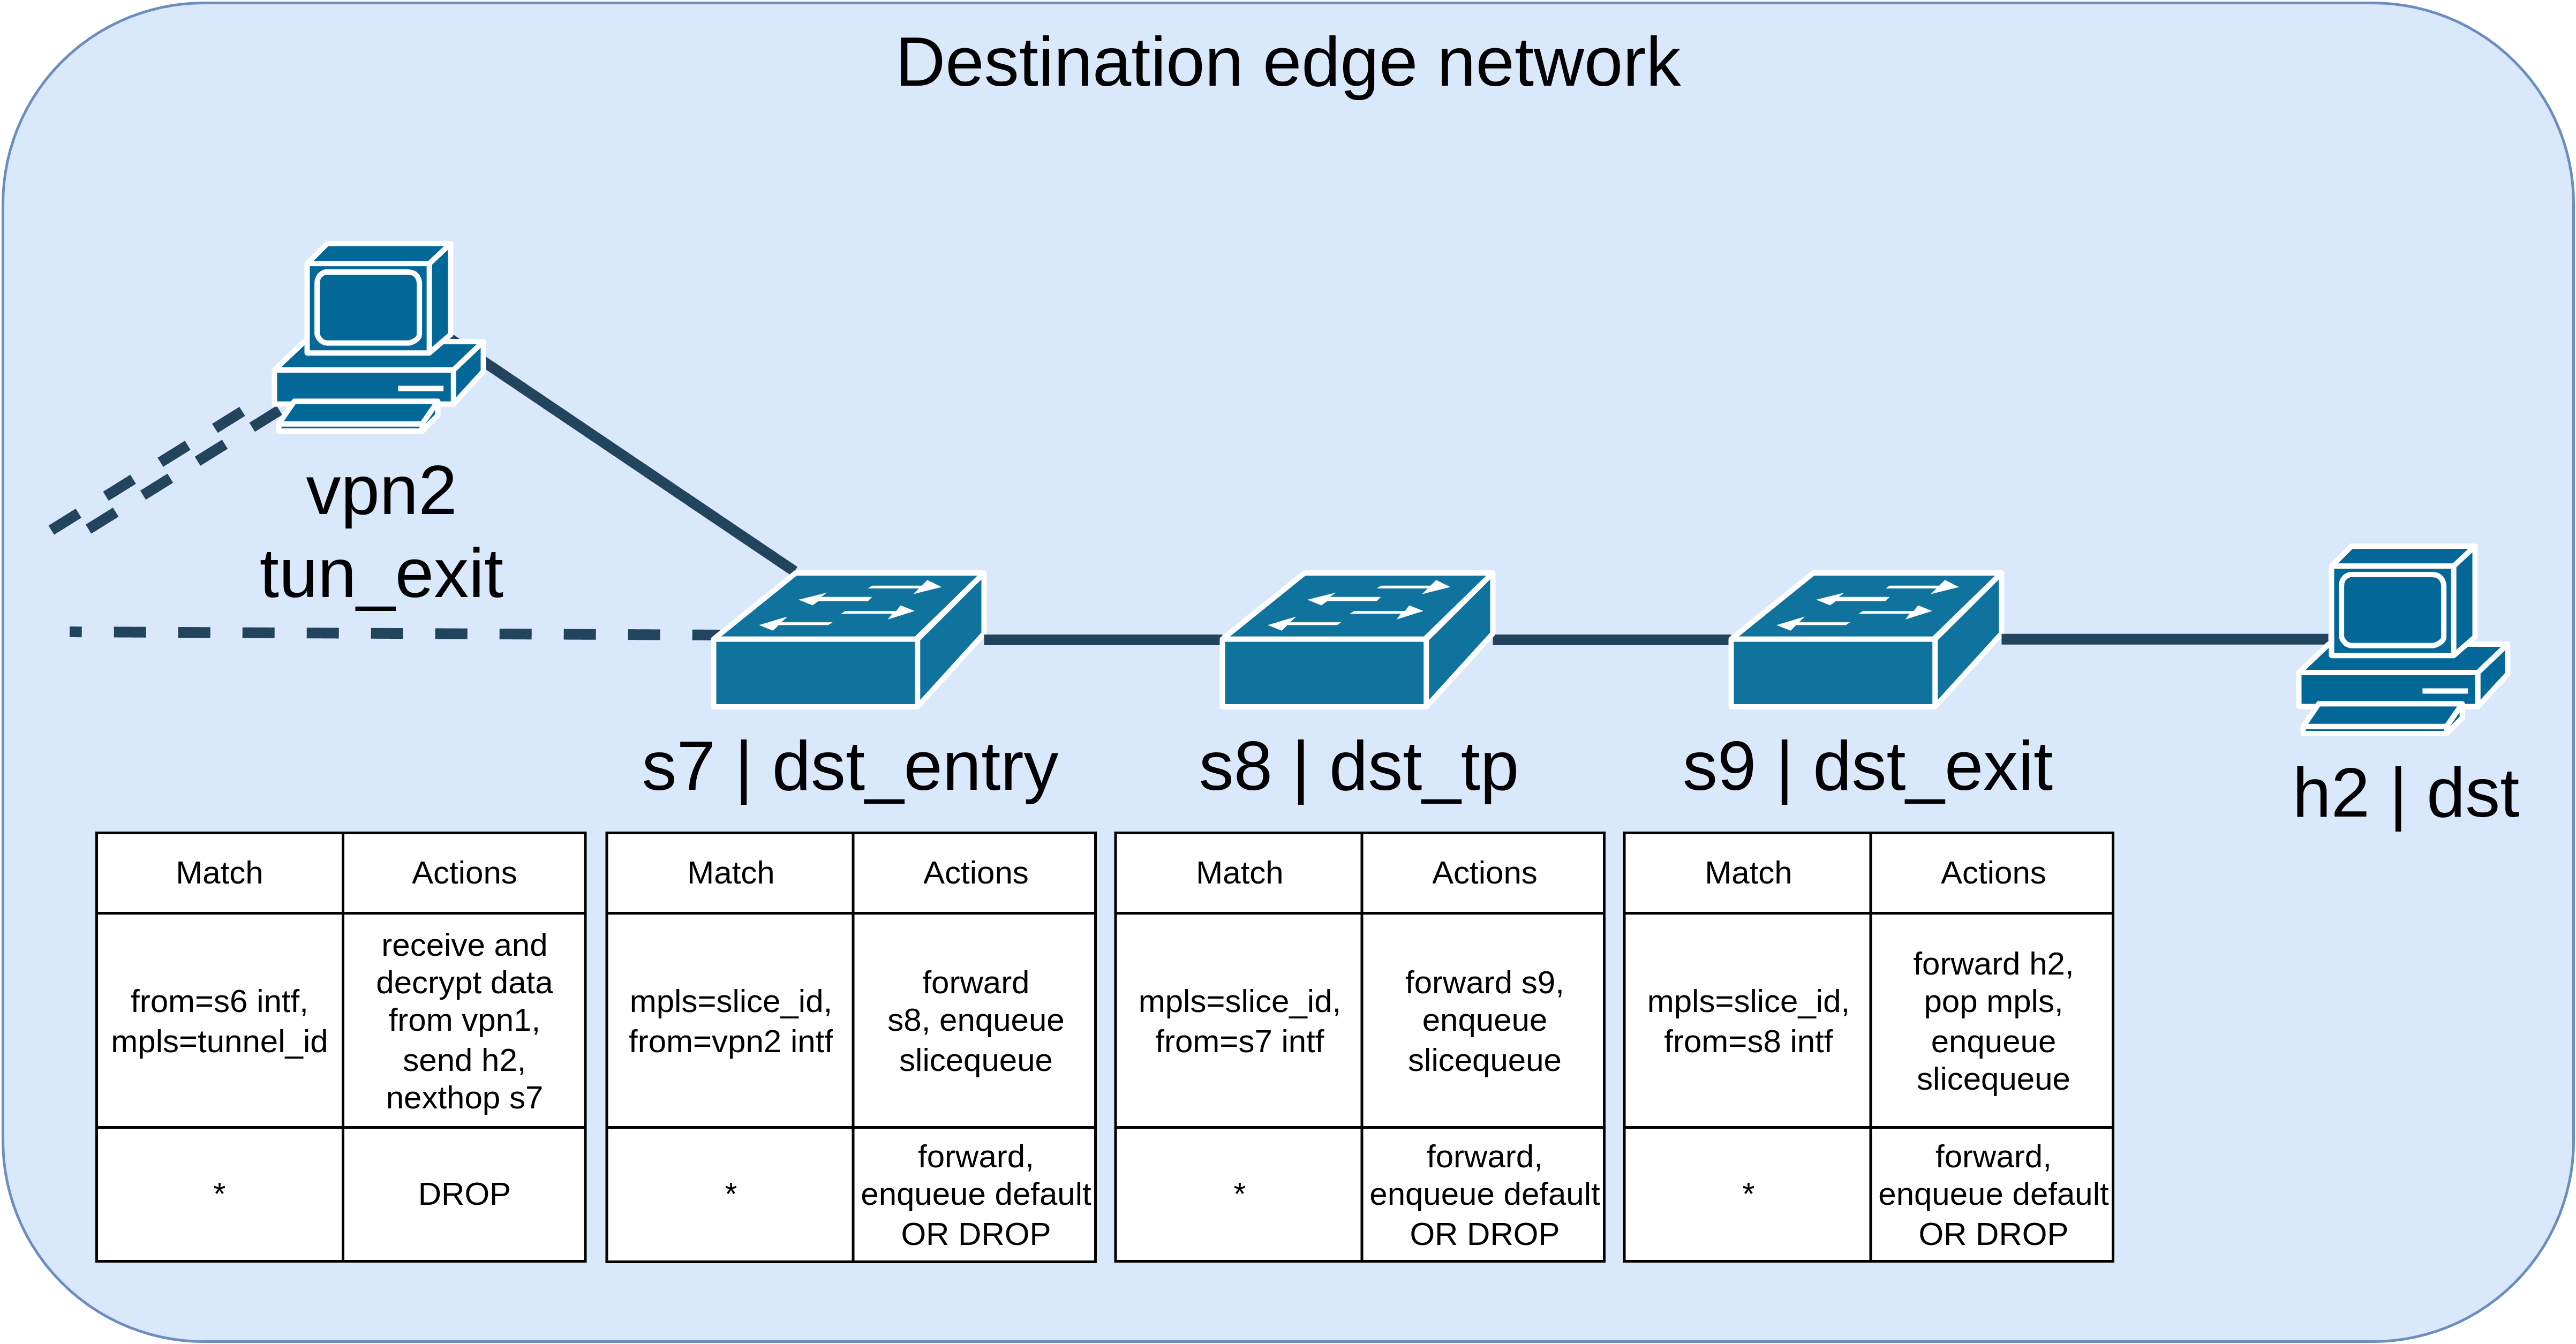
\includegraphics[width=10cm]{images/chapter_6/routing_destination.png}
    \caption[Routing on the destination \gls{edgenetwork}]{The routing rules on the destination \gls{edgenetwork} for the switches and \acrshort{vpn} gateways according to their roles. The dotted lines lead to the last \gls{blacknetwork} switch.}
    \label{fig:routing_destination}
\end{figure}

Depending on the role we then deploy the following rules (see Figure \ref{fig:routing_destination}):

\paragraph{DST\_ENTRY and DST\_TP} Will verify that a packet matches a slice by checking the slice ID \acrshort{mpls} label and the inbound interface. Will then forward the packet to the next hop.

\paragraph{DST\_ALL and DST\_EXIT} Will verify that a packet matches a slice by checking the slice ID \acrshort{mpls} label and the inbound interface. Will then remove the slice ID \acrshort{mpls} label and forward the packet to the next hop. This way the destination host will receive the original packet without any \acrshort{mpls} labels or other additional headers attached to it.

\paragraph{} All switches may also forward traffic on a default slice, where all other traffic resides. This is however not subject to our coordination and thus also not part of our implementation. The default slices will be manually configured in our validation experiments later with adequate resource limitations to not impede on our isolated slices. This feature could be added to the implementation in the future to dynamically resize the default slice and to not under-provision the traffic allocation to all other devices. Without any additional configuration currently all other traffic is blocked.

\paragraph{} As one can see, there are multiple switch roles per network that employ the same rules. This has been implemented this way to provide flexibility for future adaptations, so that potentially different routing rules can be realized in the future, where these roles would not behave identically. However there always has to be at least one switch on the source network and on the destination network before and after the \acrshort{vpn} gateway respectively.

\subsection{Tunnel configuration}
\label{impl_tunnel_config}
Concerning our tunnels we will use a similar strategy to the slices themselves, but need to allocate a tunnel entry and a tunnel exit first.

\paragraph{Tunnel entry} The tunnel entry will be created on the corresponding \acrshort{vpn} gateway on the source network. The tunnel entry will be a \gls{wireguard} tunnel that is configured in pair with the remote \gls{wireguard} tunnel entry. The tunnel entry is bound on a port that can be identified by the \gls{blacknetwork} switches later and that is assigned to the tunnel.

Because \gls{wireguard} is a layer 3 tunnel we will need to create an additional layer 2 tunnel that is established over our \gls{wireguard} tunnel to be able to forward ethernet frames through the tunnel. This has been performed by establishing a \acrshort{gre}TAP tunnel.

Now that we have our tunnel, we still need to route packets to this tunnel. This is achieved by matching packets to slices in a linux qdisc, before redirecting them to their tunnel. If no slices match, the packet will always be dropped as the \acrshort{vpn} gateways do not forward non-slice traffic. For the match only the slice ID \acrshort{mpls} label and ingress interface is evaluated, before sending the packet to the tunnel.

\paragraph{Tunnel exit} On the tunnel exit, we feature a similar approach to our tunnel entry. We thus bootstrap the tunnel counterparts, including the \gls{wireguard} and the \acrshort{gre}TAP tunnel.

When we receive a packet on the \acrshort{gre}TAP tunnel we already know which tunnel it is coming from. We then route it to the matching egress port by inspecting the slice ID \acrshort{mpls} label of the packet and thus choosing the correct egress port. The destination network will then receive the correct packet from our tunnel with the slice ID \acrshort{mpls} label remaining in place, so routing to the destination can commence.

\paragraph{} Now that we described tunnel entry and exit, the last remaining part is securing the tunnel with resource guarantees. This is performed identically to a slice, but this time all switches between the \acrshort{vpn} gateways are focused on. These switches can be on the \gls{edgenetwork}s or can be part of one of the \gls{blacknetwork}s. Any topology is possible. Compared to the slice source and destination even zero switches between the \acrshort{vpn} gateways are possible if there is only a plain link.

We will, if there are any switches, assign the same roles as with the slice source or destination, but this time the roles are prefixed with \textit{BN} for "\gls{blacknetwork}". We thus have \textit{BN\_ALL}, \textit{BN\_ENTRY}, \textit{BN\_TP} and \textit{BN\_EXIT}. First we create two queues per switch to the ingress and egress interfaces of the tunnel, one being the queue for forward traffic and the other being the queue for reverse traffic. This is required by \gls{wireguard} to perform key exchange and rotation. We only need to reserve a small amount of traffic for the reverse direction though, compared to the forward direction.

\begin{figure}[ht]
    \centering
    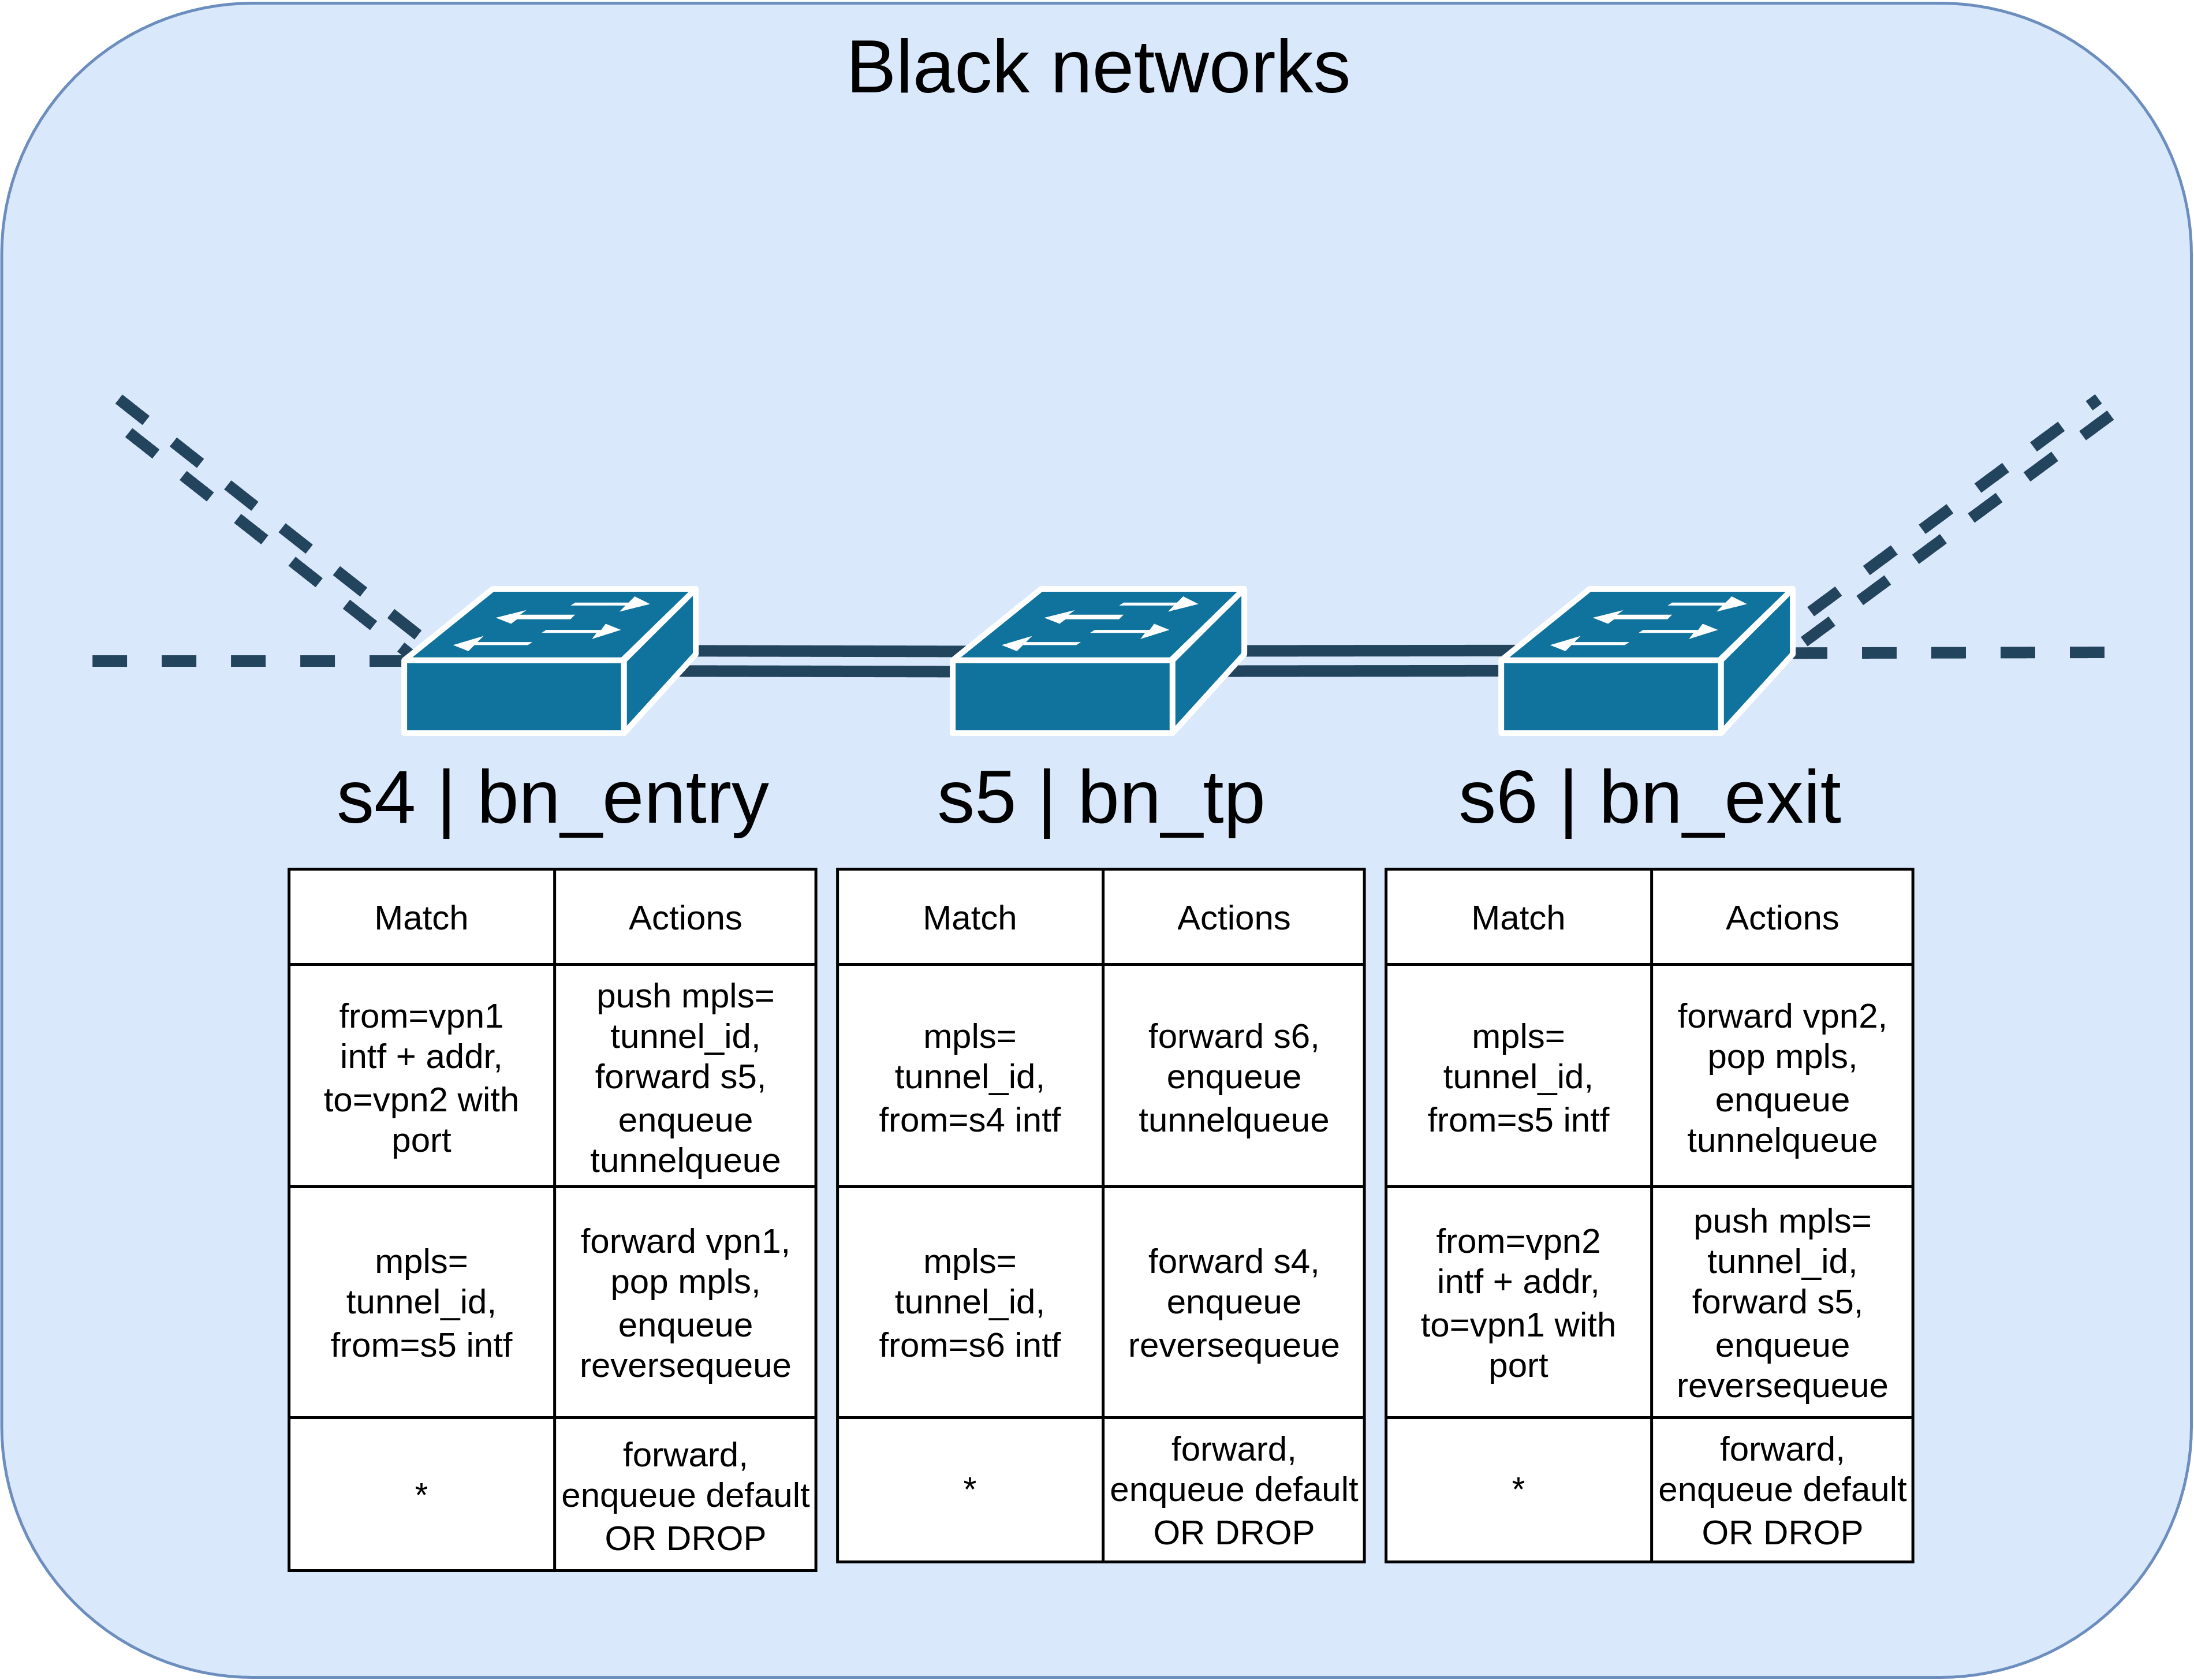
\includegraphics[width=8cm]{images/chapter_6/routing_bn.png}
    \caption[Routing on the \gls{blacknetwork}s]{The routing rules on the \gls{blacknetwork}s for the switches according to their roles. The dotted lines to the left lead to the source \gls{edgenetwork} and the dotted lines on the right lead to the destination \gls{edgenetwork}.}
    \label{fig:routing_bn}
\end{figure}

Afterwards we will establish the following rules depending on the role (see Figure \ref{fig:routing_bn}):

\paragraph{BN\_ALL} We will match all packets from both directions on the correct ingress interface for the \acrshort{udp} destination port and destination address. We will then forward traffic.

\paragraph{BN\_ENTRY} We will match all packets from the main direction on the correct ingress interface for the \acrshort{udp} destination port and IP destination address. We will then tag the packet with the tunnel ID as \acrshort{mpls} label and forward traffic.

For reverse traffic we will match for the tunnel ID \acrshort{mpls} label on the correct ingress interface. We will then remove the tunnel ID \acrshort{mpls} label and forward the traffic.

\paragraph{BN\_TP} We will match all packets from both directions on the correct ingress interface and for the tunnel ID \acrshort{mpls} label. We then forward traffic to the next hop, including the \acrshort{mpls} label.

\paragraph{BN\_EXIT} This switch will receive the reverse rules from \textit{BN\_ENTRY}. It will thus match for the tunnel ID \acrshort{mpls} label on the correct ingress interface, pop the \acrshort{mpls} label and forward the traffic to the \acrshort{vpn} gateway tunnel exit.

For the reverse direction it will match for the correct ingress interface, \acrshort{udp} port and IP destination address, before tagging the packet with the tunnel ID \acrshort{mpls} label and forwarding traffic.

\paragraph{} Concerning the traffic forwarding on a default slice, the same applies as with the source and destination \gls{edgenetwork}s. Please note however that the \acrshort{vpn} gateways will never forward any traffic. Therefore, routing of a default slice (when configured manually) has to be routed around the \acrshort{vpn} gateways, for example by using a different link between a \textit{SRC\_EXIT} and \textit{BN\_ENTRY} switch (or other valid combinations).


\section{Lessons learned}
Of course we encountered some issues while implementing our solution. We will discuss them here and present their solution, so that future developers will not face the same issues. We will begin with MTU considerations and \acrshort{mpls} label popping in \Gls{openflow}, before presenting checksum offloading issues and write queue overflows in the linux kernel.

%\cgn{Maybe instead of Challenges, change the heading to Lessons learned. Challenges sound like unsolved problems. However, in this case you faced issues and had solutions for those.}

\subsection{MTU considerations}
Maybe one of the most obvious issues are MTU considerations. Our multiple \acrshort{mpls} and \acrshort{gre}TAP headers (see Figure \ref{fig:packet_structure}) will attach information to packets, alongside the additional encapsulation by \gls{wireguard}. When packets get close to the network MTU in size, this can lead to fragmentation of packets that would otherwise fit in the MTU. In our case, packets would no longer be delivered after being fragmented. To combat this, a lower MTU than the network MTU should be applied on the hosts. We chose 1300 in our host \acrshort{lxc} container image, which is 200 byte smaller than the network MTU. Slightly higher values might be possible, but this has not been investigated.

\begin{figure}[hp]
    \centering
    \includegraphics[width=10cm]{images/chapter_6/packet_structure.png}
    \caption[Additional headers of packets]{This figure shows the additional headers that a packet receives while traveling through our architecture according to the routing rules specified in Section \ref{impl_concepts}. These additional headers decrease our MTU for packets that we can accept. Our payload is in white, layer two to four headers in red and \acrshort{mpls} headers are in blue. Gray is used to indicate encrypted content within the \gls{wireguard} tunnel, acting as a payload for the tunnel.}
    \label{fig:packet_structure}
\end{figure}

\subsection{MPLS label popping in OpenFlow}
Headaches have been caused due to the \acrshort{mpls} label popping implemented in \Gls{openflow}. The author assumed, that when popping an \acrshort{mpls} label, one has to submit the \acrshort{mpls} label ID that should be popped. This would make sense because it is possible to stack multiple \acrshort{mpls} labels and maybe the second or third in the stack should get popped. This is however not the case. Instead one has to specify the \gls{ethertype} of the resulting packet \cite{openflow}, which would be 2048 (or 0x800) for \acrshort{ipv4} \cite{rfc7042}. This caused corrupt packets on the destination host.

\subsection{Checksum offloading issues}
Another issue with corrupt packets on the destination host was caused by invalid \acrshort{udp} and \acrshort{tcp} checksums. When pushing or popping \acrshort{mpls} labels, current implementations of \Gls{ovs} break the \acrshort{udp} and \acrshort{tcp} checksums while \acrshort{tx} (write) offloading is enabled on the switch interfaces. To fix the checksum calculations, one has to disable \acrshort{tx} offloading on all switch interfaces like this:

\begin{lstlisting}[language=bash]
ethtool --offload $INTF_NAME tx off
\end{lstlisting}

More information on this can be found in the linux kernel documentation \cite{txoffload}.

\subsection{Write queue overflow}
While testing our slicing architecture under a flooding attack locally, we noticed that packets were being dropped on the \acrshort{vpn} gateway. We decided to investigate this in more detail, because traffic from the adversaries was not even flowing through the \acrshort{vpn} gateways, but would rather flow around them (as described in Section \ref{impl_tunnel_config}). This was very unexpected for us in the beginning. We noticed that packets were received by the \acrshort{vpn} gateway, but were dropped on the tunnel interface before entering the \gls{wireguard} tunnel.

Our first measure was to increase the \acrshort{tx} (write) queue size, which improved the result but still saw dropped packets. After trying some other approaches which all failed to solve the problem, we finally found the solution.

By pinning the adversaries to certain CPU threads that they can use, the \acrshort{tx} queue would no longer overflow. It was interesting that we could even pin the attackers to all but one thread to stop packets from dropping. We currently assume that this happens due to CPU spikes caused by the adversaries while using \textit{hping3}, which stole enough computational time from the \acrshort{vpn} gateways to make them drop packets.

Subsequently we stuck to the CPU pinning of the attackers, but still assigned all but one or two threads to them which should have next to negligible impact and is more than generous (30 out of 32 threads and 3 out of 4 threads in our tests). This is also a realistic approach, as usually in a real-world network, attackers would not share the same CPU with our switches or \acrshort{vpn} gateways. However this may not always be the case in container setups. An easy solution to this could be to apply resource limits to containers as is common practice in modern setups.

\chapter{Validation}
For each experiment:
\begin{itemize}
    \item Outcome of the experiment
    \item Is it the outcome we expected?
\end{itemize}
\chapter{Conclusion}
\label{conclusion}
\iffalse
\begin{itemize}
    \item Summary
    \item Limitations
    \item Future work
\end{itemize}
\fi

Isolation of tenants is one of the key requirements for building a network based on the zero trust approach \cite{zerotrust}, which has become more and more relevant due to the increase of devices in IoT \cite{iotincrease} and the subsequently increasing threats to network architectures \cite{iotthreats}. Network slicing can be used to isolate certain devices on a network which has gained additional popularity since the advent of 5G \cite{5G1, 5G2, 5G3}, of which network slicing is an integral part.

In this thesis we designed and implemented a solution to create isolated network slices across multiple domains and evaluated it for our protection goals of confidentiality, integrity, availability and resilience. This has been performed by conducting carefully designed experiments against multiple different scenarios that resemble real-world network architectures. Part of these scenarios is also one distributed scenario, where individual domains are separated on individual network nodes, integrating a hardware switch for some performance measurements that are closer to the real-world behaviour of switches.

Apart from meeting these requirements, our proposed solution also features distributed coordination of network slices allowing multiple domains to work together without necessarily trusting each other. This enables us to work together with other parties to bootstrap network  slices over multiple networks. Furthermore our solution has been built with compatibility in mind by separating components, using common standards like OpenFlow and providing specifiactions for our APIs. We also provide flexibility of network slices, allowing tenants to request multiple slices to multiple different target domains

Considering our initial example of a remote surgery robot, we can thus confidently state that the connection from the surgeon to the robot would provide significantly more resistance against attacks than before and as of now, the connection could not be broken by our attackers. For a patient, this can mean a better and longer life as opposed to the consequences of failure in a surgery.

\section{Limitations}
As with any solution, there are some limitations though. First, only two tenants may be part of a network slice, because a network slice is a communication channel in our solution. To include more tenants one can always build a mesh of communication channels though.

Closely related to this is that currently, network slices are always expected to go to another domain. Requesting a slice to the own local domain is not possible however. This functionality could be implemented in the future though.

A bigger limitation is currently, that we do not pass protection goals for availability and resilience if domain coordinators are attacked by HTTP floods or other DoS methods. This could be mitigated by protecting the coordinators against these attacks from their tenants, for example by deploying anti DoS solutions and firewalls. This has not been investigated however.

\section{Future work}
Many different things would come to mind when thinking about potential future work. One direction would be progressing the implementation further to production readiness. Requirements for this would be resilience against DoS on the coordinators, a proper authentication scheme and implementation of our VNFs for vendor specific hardware. Furthermore our APIs would need to be protected for attacks on confidentiality and integrity, for example by deploying TLS to all services. Also more validation on API endpoints could be performed in advance, so that requests can be rejected earlier before even asking other services to perform changes or running into errors.

Furthermore our implementation currently does not validate the successful creation and deletion of flows on the switches. This would need to be confirmed by a production-ready solution. While we were confident that OpenFlow (UDP) messages would not get lost on their way from the controllers to the switches in our test scenarios, this may not hold true in reality.

The tunnel allocation logic could also be adapted to match the needs of the individual networks more closely. This could also incorporate sending a single packet on allocation to force the tunnel handshake so the initial packets of a tunnel get delivered faster.

The second direction would be progressing more on features. One feature could be accounting, where tenants would invest a currency to establish and keep a slice. This could either be used for billing these tenants or to allocate communication contingents to them apart from the already implemented parallel resource allocation limits. This is for example already common practice in mobile broadband.

Apart from this, another feature could be to set time limits on slices upon allocation, so that slices get removed automatically after a specified time or if they have not been used in a while. This could help limit a potential overflow in our slicing architecture after some time of operation.

Lastly, another interesting option to explore would be to actually factor in the latency with our architecture. Currently, the architecture just provides the best latency that it can offer by choosing and securing the shortest path if possible. In the future the latency requirements could be factored in to choose an appropriate path through the network that can deliver the required latency but might be under less load.

\listoffigures
\cts{when making tables/lists of content, please use $caption\{\}[]$ with short captions for the TOC :)}
\listoftables

\printbibliography[heading=bibintoc, notkeyword={usedtools}]

\printbibliography[heading=bibintoc, keyword={usedtools}, title={Tool references}]

\appendix

\chapter{Specifications}
\label{specifications}

%\section{ESMF}
\label{spec_esmf}

A simple API to interact with the Edge Slice Management Function. Supports creating and removing slices across domains. Synchronises itself with other ESMFs to achieve a common goal. Please refer to the topology drawings for further information about the network structures.

\subsection{Authentication}
\subsubsection{POST /auth}
Issues a new authentication token in exchange for credentials. Currently requires no credentials, this is up to future implementations.
\begin{longtable}{ |p{2.5cm}|p{1.5cm}|p{4cm}|p{2cm}| }
\hline
\multicolumn{4}{|c|}{\textbf{Parameters}} \\
 \hline
\multicolumn{4}{|p{11.34cm}|}{\centering{\textit{No parameters}}} \\
 \hline
\endhead \end{longtable}

\begin{longtable}{ |p{3cm}|p{7.88cm}| }
\hline
\multicolumn{2}{|c|}{\textbf{Request Body}} \\
 \hline
\multicolumn{2}{|p{11.34cm}|}{\centering{\textit{No request body}}} \\
 \hline \endhead
\end{longtable}

\begin{longtable}{ |p{1.0cm}|p{3cm}|p{6.44cm}| }
\hline
\multicolumn{3}{|c|}{\textbf{Responses}} \\
 \hline
\centering{\textbf{Code}} & \centering{\textbf{Content Type}} & \textbf{Description, Data Type} \\
\hline
\centering{200} & \centering{application/json} & The authentication token as string

\paragraph{Data} string \\
 \hline
\endhead
\centering{403} & \centering{text/plain} & Wrong credentials were specified \\
 \hline
\end{longtable}

\newpage
\subsection{Slice Management}
\subsubsection{GET /slice}
Lists all current slices by this requester. This endpoint is only available on ESMFs.
\begin{longtable}{ |p{2.5cm}|p{1.5cm}|p{4cm}|p{2cm}| }
\hline
\multicolumn{4}{|c|}{\textbf{Parameters}} \\
 \hline
\textbf{Name} & \centering{\textbf{Location}} & \textbf{Description} & \textbf{Type} \\
\hline
auth & \centering{QUERY} & The authentication token issued by prior login & string \\
 \hline
\endhead \end{longtable}

\begin{longtable}{ |p{3cm}|p{7.88cm}| }
\hline
\multicolumn{2}{|c|}{\textbf{Request Body}} \\
 \hline
\multicolumn{2}{|p{11.34cm}|}{\centering{\textit{No request body}}} \\
 \hline \endhead
\end{longtable}

\begin{longtable}{ |p{1.0cm}|p{3cm}|p{6.44cm}| }
\hline
\multicolumn{3}{|c|}{\textbf{Responses}} \\
 \hline
\centering{\textbf{Code}} & \centering{\textbf{Content Type}} & \textbf{Description, Data Type} \\
\hline
\centering{200} & \centering{application/json} & The current list of slices assigned to this requester

\paragraph{Data} [\hyperref[esmf_slice]{slice}] \\
 \hline
\endhead
\centering{403} & \centering{text/plain} & Invalid authentication provided \\
 \hline
\centering{421} & \centering{text/plain} & Slice management is not supported by this service \\
 \hline
\end{longtable}

\newpage
\subsubsection{PUT /slice}
Creates one or multiple new slices from one host to another. Will either create all slices if feasible or none at all. This endpoint is only available on ESMFs.
\begin{longtable}{ |p{2.5cm}|p{1.5cm}|p{4cm}|p{2cm}| }
\hline
\multicolumn{4}{|c|}{\textbf{Parameters}} \\
 \hline
\textbf{Name} & \centering{\textbf{Location}} & \textbf{Description} & \textbf{Type} \\
\hline
auth & \centering{QUERY} & The authentication token issued by prior login & string \\
 \hline
\endhead \end{longtable}

\begin{longtable}{ |p{3cm}|p{7.88cm}| }
\hline
\multicolumn{2}{|c|}{\textbf{Request Body}} \\
 \hline
\textbf{Content Type} & \textbf{Data Type} \\
\hline
application/json & [\hyperref[esmf_slice]{slice}] \\
 \hline
\end{longtable}

\begin{longtable}{ |p{1.0cm}|p{3cm}|p{6.44cm}| }
\hline
\multicolumn{3}{|c|}{\textbf{Responses}} \\
 \hline
\centering{\textbf{Code}} & \centering{\textbf{Content Type}} & \textbf{Description, Data Type} \\
\hline
\centering{200} & \centering{application/json} & The slices have been deployed. Returns the parameters of the deployed slices, including the fresh ids.

\paragraph{Data} [\hyperref[esmf_slice]{slice}] \\
 \hline
\endhead
\centering{403} & \centering{text/plain} & Invalid or insufficient authentication provided \\
 \hline
\centering{404} & \centering{text/plain} & The input or output of one or multiple of the slices could not be found \\
 \hline
\centering{417} & \centering{text/plain} & No slices were requested \\
 \hline
\centering{421} & \centering{text/plain} & Slice management is not supported by this service \\
 \hline
\centering{422} & \centering{text/plain} & Can not handle slices not originating from or to our network \\
 \hline
\centering{429} & \centering{text/plain} & Please slow down. You may only use slice actions every couple of seconds. \\
 \hline
\centering{500} & \centering{text/plain} & Internal error \\
 \hline
\centering{507} & \centering{text/plain} & Insufficient resources by participating domain or requester \\
 \hline
\end{longtable}

\newpage
\subsubsection{DELETE /slice}
Deletes one or multiple slices. This endpoint is only available on ESMFs.
\begin{longtable}{ |p{2.5cm}|p{1.5cm}|p{4cm}|p{2cm}| }
\hline
\multicolumn{4}{|c|}{\textbf{Parameters}} \\
 \hline
\textbf{Name} & \centering{\textbf{Location}} & \textbf{Description} & \textbf{Type} \\
\hline
auth & \centering{QUERY} & The authentication token issued by prior login & string \\
 \hline
slice\_ids & \centering{QUERY} & The ids of the slices to be deleted. & [integer/int32] \\
 \hline
\endhead \end{longtable}

\begin{longtable}{ |p{3cm}|p{7.88cm}| }
\hline
\multicolumn{2}{|c|}{\textbf{Request Body}} \\
 \hline
\multicolumn{2}{|p{11.34cm}|}{\centering{\textit{No request body}}} \\
 \hline \endhead
\end{longtable}

\begin{longtable}{ |p{1.0cm}|p{3cm}|p{6.44cm}| }
\hline
\multicolumn{3}{|c|}{\textbf{Responses}} \\
 \hline
\centering{\textbf{Code}} & \centering{\textbf{Content Type}} & \textbf{Description, Data Type} \\
\hline
\centering{200} & \centering{text/plain} & The slices were successfully deleted. \\
 \hline
\endhead
\centering{403} & \centering{text/plain} & Invalid or insufficient authentication provided. \\
 \hline
\centering{404} & \centering{text/plain} & One or multiple of the slices could not be found. \\
 \hline
\centering{417} & \centering{text/plain} & No slice ids were provided. \\
 \hline
\centering{421} & \centering{text/plain} & Slice management is not supported by this service \\
 \hline
\centering{429} & \centering{text/plain} & Please slow down. You may only use slice actions every couple of seconds. \\
 \hline
\centering{500} & \centering{text/plain} & Internal error \\
 \hline
\end{longtable}

\newpage
\subsection{Configuration}
\subsubsection{GET /configuration}
Fetch the current configuration of this service
\begin{longtable}{ |p{2.5cm}|p{1.5cm}|p{4cm}|p{2cm}| }
\hline
\multicolumn{4}{|c|}{\textbf{Parameters}} \\
 \hline
\textbf{Name} & \centering{\textbf{Location}} & \textbf{Description} & \textbf{Type} \\
\hline
auth & \centering{QUERY} & The authentication token issued by prior login & string \\
 \hline
\endhead \end{longtable}

\begin{longtable}{ |p{3cm}|p{7.88cm}| }
\hline
\multicolumn{2}{|c|}{\textbf{Request Body}} \\
 \hline
\multicolumn{2}{|p{11.34cm}|}{\centering{\textit{No request body}}} \\
 \hline \endhead
\end{longtable}

\begin{longtable}{ |p{1.0cm}|p{3cm}|p{6.44cm}| }
\hline
\multicolumn{3}{|c|}{\textbf{Responses}} \\
 \hline
\centering{\textbf{Code}} & \centering{\textbf{Content Type}} & \textbf{Description, Data Type} \\
\hline
\centering{200} & \centering{application/json} & The current configuration

\paragraph{Data} \hyperref[esmf_domain_configuration]{domain\_configuration} \\
 \hline
\endhead
\centering{403} & \centering{text/plain} & Invalid authentication provided \\
 \hline
\end{longtable}

\newpage
\subsubsection{PUT /configuration}
Installs a new configuration for this service
\begin{longtable}{ |p{2.5cm}|p{1.5cm}|p{4cm}|p{2cm}| }
\hline
\multicolumn{4}{|c|}{\textbf{Parameters}} \\
 \hline
\textbf{Name} & \centering{\textbf{Location}} & \textbf{Description} & \textbf{Type} \\
\hline
auth & \centering{QUERY} & The authentication token issued by prior login & string \\
 \hline
\endhead \end{longtable}

\begin{longtable}{ |p{3cm}|p{7.88cm}| }
\hline
\multicolumn{2}{|c|}{\textbf{Request Body}} \\
 \hline
\textbf{Content Type} & \textbf{Data Type} \\
\hline
application/json & \hyperref[esmf_domain_configuration]{domain\_configuration} \\
 \hline
\end{longtable}

\begin{longtable}{ |p{1.0cm}|p{3cm}|p{6.44cm}| }
\hline
\multicolumn{3}{|c|}{\textbf{Responses}} \\
 \hline
\centering{\textbf{Code}} & \centering{\textbf{Content Type}} & \textbf{Description, Data Type} \\
\hline
\centering{200} & \centering{text/plain} & The configuration has been installed \\
 \hline
\endhead
\centering{403} & \centering{text/plain} & Invalid authentication provided \\
 \hline
\centering{406} & \centering{text/plain} & A value exceeds the allowed range \\
 \hline
\centering{409} & \centering{text/plain} & There are slices currently running. Reconfiguring is not supported while slices are open. \\
 \hline
\centering{412} & \centering{text/plain} & The provided configuration is invalid \\
 \hline
\end{longtable}

\newpage
\subsection{Slice Synchronization}
\subsubsection{GET /slice\_reservation}
Lists all current slice reservations. This endpoint is only available on ESMFs.
\begin{longtable}{ |p{2.5cm}|p{1.5cm}|p{4cm}|p{2cm}| }
\hline
\multicolumn{4}{|c|}{\textbf{Parameters}} \\
 \hline
\textbf{Name} & \centering{\textbf{Location}} & \textbf{Description} & \textbf{Type} \\
\hline
auth & \centering{QUERY} & The authentication token issued by prior login & string \\
 \hline
\endhead \end{longtable}

\begin{longtable}{ |p{3cm}|p{7.88cm}| }
\hline
\multicolumn{2}{|c|}{\textbf{Request Body}} \\
 \hline
\multicolumn{2}{|p{11.34cm}|}{\centering{\textit{No request body}}} \\
 \hline \endhead
\end{longtable}

\begin{longtable}{ |p{1.0cm}|p{3cm}|p{6.44cm}| }
\hline
\multicolumn{3}{|c|}{\textbf{Responses}} \\
 \hline
\centering{\textbf{Code}} & \centering{\textbf{Content Type}} & \textbf{Description, Data Type} \\
\hline
\centering{200} & \centering{application/json} & The current list of slice reservations

\paragraph{Data} [\hyperref[esmf_slice]{slice}] \\
 \hline
\endhead
\centering{403} & \centering{text/plain} & Invalid authentication provided \\
 \hline
\centering{421} & \centering{text/plain} & Slice management is not supported by this service \\
 \hline
\end{longtable}

\newpage
\subsubsection{PUT /slice\_reservation}
Creates a new slice reservation. This endpoint is only available on ESMFs.
\begin{longtable}{ |p{2.5cm}|p{1.5cm}|p{4cm}|p{2cm}| }
\hline
\multicolumn{4}{|c|}{\textbf{Parameters}} \\
 \hline
\textbf{Name} & \centering{\textbf{Location}} & \textbf{Description} & \textbf{Type} \\
\hline
auth & \centering{QUERY} & The authentication token issued by prior login & string \\
 \hline
\endhead \end{longtable}

\begin{longtable}{ |p{3cm}|p{7.88cm}| }
\hline
\multicolumn{2}{|c|}{\textbf{Request Body}} \\
 \hline
\textbf{Content Type} & \textbf{Data Type} \\
\hline
application/json & \hyperref[esmf_slice]{slice} \\
 \hline
\end{longtable}

\begin{longtable}{ |p{1.0cm}|p{3cm}|p{6.44cm}| }
\hline
\multicolumn{3}{|c|}{\textbf{Responses}} \\
 \hline
\centering{\textbf{Code}} & \centering{\textbf{Content Type}} & \textbf{Description, Data Type} \\
\hline
\centering{200} & \centering{text/plain} & The slice has been reserved \\
 \hline
\endhead
\centering{403} & \centering{text/plain} & Invalid authentication provided \\
 \hline
\centering{404} & \centering{text/plain} & The input or output could not be found \\
 \hline
\centering{406} & \centering{text/plain} & A value exceeds the allowed range \\
 \hline
\centering{409} & \centering{text/plain} & A slice with this id is already known \\
 \hline
\centering{412} & \centering{text/plain} & A value does not match the schema \\
 \hline
\centering{421} & \centering{text/plain} & Slice management is not supported by this service \\
 \hline
\centering{500} & \centering{text/plain} & Internal error \\
 \hline
\centering{507} & \centering{text/plain} & Insufficient resources \\
 \hline
\end{longtable}

\newpage
\subsubsection{DELETE /slice\_reservation}
Deletes a slice reservation. This endpoint is only available on ESMFs.
\begin{longtable}{ |p{2.5cm}|p{1.5cm}|p{4cm}|p{2cm}| }
\hline
\multicolumn{4}{|c|}{\textbf{Parameters}} \\
 \hline
\textbf{Name} & \centering{\textbf{Location}} & \textbf{Description} & \textbf{Type} \\
\hline
auth & \centering{QUERY} & The authentication token issued by prior login & string \\
 \hline
slice\_id & \centering{QUERY} & The id of the slice reservation to be deleted. & integer/int32 \\
 \hline
\endhead \end{longtable}

\begin{longtable}{ |p{3cm}|p{7.88cm}| }
\hline
\multicolumn{2}{|c|}{\textbf{Request Body}} \\
 \hline
\multicolumn{2}{|p{11.34cm}|}{\centering{\textit{No request body}}} \\
 \hline \endhead
\end{longtable}

\begin{longtable}{ |p{1.0cm}|p{3cm}|p{6.44cm}| }
\hline
\multicolumn{3}{|c|}{\textbf{Responses}} \\
 \hline
\centering{\textbf{Code}} & \centering{\textbf{Content Type}} & \textbf{Description, Data Type} \\
\hline
\centering{200} & \centering{text/plain} & The slice reservation was successfully deleted. \\
 \hline
\endhead
\centering{403} & \centering{text/plain} & Invalid authentication provided. \\
 \hline
\centering{404} & \centering{text/plain} & The slice reservation could not be found. \\
 \hline
\centering{421} & \centering{text/plain} & Slice management is not supported by this service \\
 \hline
\centering{500} & \centering{text/plain} & Internal error \\
 \hline
\end{longtable}

\newpage
\subsubsection{GET /slice\_deployment}
Lists all current slices. This endpoint is only available on ESMFs.
\begin{longtable}{ |p{2.5cm}|p{1.5cm}|p{4cm}|p{2cm}| }
\hline
\multicolumn{4}{|c|}{\textbf{Parameters}} \\
 \hline
\textbf{Name} & \centering{\textbf{Location}} & \textbf{Description} & \textbf{Type} \\
\hline
auth & \centering{QUERY} & The authentication token issued by prior login & string \\
 \hline
\endhead \end{longtable}

\begin{longtable}{ |p{3cm}|p{7.88cm}| }
\hline
\multicolumn{2}{|c|}{\textbf{Request Body}} \\
 \hline
\multicolumn{2}{|p{11.34cm}|}{\centering{\textit{No request body}}} \\
 \hline \endhead
\end{longtable}

\begin{longtable}{ |p{1.0cm}|p{3cm}|p{6.44cm}| }
\hline
\multicolumn{3}{|c|}{\textbf{Responses}} \\
 \hline
\centering{\textbf{Code}} & \centering{\textbf{Content Type}} & \textbf{Description, Data Type} \\
\hline
\centering{200} & \centering{application/json} & The current list of slices

\paragraph{Data} [\hyperref[esmf_slice]{slice}] \\
 \hline
\endhead
\centering{403} & \centering{text/plain} & Invalid authentication provided \\
 \hline
\centering{421} & \centering{text/plain} & Slice management is not supported by this service \\
 \hline
\end{longtable}

\newpage
\subsubsection{PUT /slice\_deployment}
Creates a new slice from a reservation. This endpoint is only available on ESMFs.
\begin{longtable}{ |p{2.5cm}|p{1.5cm}|p{4cm}|p{2cm}| }
\hline
\multicolumn{4}{|c|}{\textbf{Parameters}} \\
 \hline
\textbf{Name} & \centering{\textbf{Location}} & \textbf{Description} & \textbf{Type} \\
\hline
auth & \centering{QUERY} & The authentication token issued by prior login & string \\
 \hline
slice\_id & \centering{QUERY} & The slice to create from the corresponding reservation id & integer/int32 \\
 \hline
\endhead \end{longtable}

\begin{longtable}{ |p{3cm}|p{7.88cm}| }
\hline
\multicolumn{2}{|c|}{\textbf{Request Body}} \\
 \hline
\multicolumn{2}{|p{11.34cm}|}{\centering{\textit{No request body}}} \\
 \hline \endhead
\end{longtable}

\begin{longtable}{ |p{1.0cm}|p{3cm}|p{6.44cm}| }
\hline
\multicolumn{3}{|c|}{\textbf{Responses}} \\
 \hline
\centering{\textbf{Code}} & \centering{\textbf{Content Type}} & \textbf{Description, Data Type} \\
\hline
\centering{200} & \centering{text/plain} & The slice has been created \\
 \hline
\endhead
\centering{403} & \centering{text/plain} & Invalid authentication provided \\
 \hline
\centering{404} & \centering{text/plain} & The slice reservation could not be found. \\
 \hline
\centering{412} & \centering{text/plain} & The tunnel referenced by this slice has not been deployed yet \\
 \hline
\centering{421} & \centering{text/plain} & Slice management is not supported by this service \\
 \hline
\centering{500} & \centering{text/plain} & The deployment to the network failed \\
 \hline
\end{longtable}

\newpage
\subsubsection{DELETE /slice\_deployment}
Deletes a slice. This endpoint is only available on ESMFs.
\begin{longtable}{ |p{2.5cm}|p{1.5cm}|p{4cm}|p{2cm}| }
\hline
\multicolumn{4}{|c|}{\textbf{Parameters}} \\
 \hline
\textbf{Name} & \centering{\textbf{Location}} & \textbf{Description} & \textbf{Type} \\
\hline
auth & \centering{QUERY} & The authentication token issued by prior login & string \\
 \hline
slice\_id & \centering{QUERY} & The id of the slice to be deleted. & integer/int32 \\
 \hline
\endhead \end{longtable}

\begin{longtable}{ |p{3cm}|p{7.88cm}| }
\hline
\multicolumn{2}{|c|}{\textbf{Request Body}} \\
 \hline
\multicolumn{2}{|p{11.34cm}|}{\centering{\textit{No request body}}} \\
 \hline \endhead
\end{longtable}

\begin{longtable}{ |p{1.0cm}|p{3cm}|p{6.44cm}| }
\hline
\multicolumn{3}{|c|}{\textbf{Responses}} \\
 \hline
\centering{\textbf{Code}} & \centering{\textbf{Content Type}} & \textbf{Description, Data Type} \\
\hline
\centering{200} & \centering{text/plain} & The slice was successfully deleted. \\
 \hline
\endhead
\centering{403} & \centering{text/plain} & Invalid authentication provided. \\
 \hline
\centering{404} & \centering{text/plain} & The slice could not be found. \\
 \hline
\centering{421} & \centering{text/plain} & Slice management is not supported by this service \\
 \hline
\centering{500} & \centering{text/plain} & The deployment to the network failed \\
 \hline
\end{longtable}

\newpage
\subsection{Tunnel Synchronization}
\subsubsection{GET /tunnel\_reservation}
Lists all current tunnel reservations
\begin{longtable}{ |p{2.5cm}|p{1.5cm}|p{4cm}|p{2cm}| }
\hline
\multicolumn{4}{|c|}{\textbf{Parameters}} \\
 \hline
\textbf{Name} & \centering{\textbf{Location}} & \textbf{Description} & \textbf{Type} \\
\hline
auth & \centering{QUERY} & The authentication token issued by prior login & string \\
 \hline
\endhead \end{longtable}

\begin{longtable}{ |p{3cm}|p{7.88cm}| }
\hline
\multicolumn{2}{|c|}{\textbf{Request Body}} \\
 \hline
\multicolumn{2}{|p{11.34cm}|}{\centering{\textit{No request body}}} \\
 \hline \endhead
\end{longtable}

\begin{longtable}{ |p{1.0cm}|p{3cm}|p{6.44cm}| }
\hline
\multicolumn{3}{|c|}{\textbf{Responses}} \\
 \hline
\centering{\textbf{Code}} & \centering{\textbf{Content Type}} & \textbf{Description, Data Type} \\
\hline
\centering{200} & \centering{application/json} & The current list of tunnel reservations

\paragraph{Data} [\hyperref[esmf_tunnel]{tunnel}] \\
 \hline
\endhead
\centering{403} & \centering{text/plain} & Invalid authentication provided \\
 \hline
\end{longtable}

\newpage
\subsubsection{PUT /tunnel\_reservation}
Creates a new tunnel reservation or stages changes to an existing deployed tunnel, as long as source and target of the tunnel match.
\begin{longtable}{ |p{2.5cm}|p{1.5cm}|p{4cm}|p{2cm}| }
\hline
\multicolumn{4}{|c|}{\textbf{Parameters}} \\
 \hline
\textbf{Name} & \centering{\textbf{Location}} & \textbf{Description} & \textbf{Type} \\
\hline
auth & \centering{QUERY} & The authentication token issued by prior login & string \\
 \hline
\endhead \end{longtable}

\begin{longtable}{ |p{3cm}|p{7.88cm}| }
\hline
\multicolumn{2}{|c|}{\textbf{Request Body}} \\
 \hline
\textbf{Content Type} & \textbf{Data Type} \\
\hline
application/json & \hyperref[esmf_tunnel]{tunnel} \\
 \hline
\end{longtable}

\begin{longtable}{ |p{1.0cm}|p{3cm}|p{6.44cm}| }
\hline
\multicolumn{3}{|c|}{\textbf{Responses}} \\
 \hline
\centering{\textbf{Code}} & \centering{\textbf{Content Type}} & \textbf{Description, Data Type} \\
\hline
\centering{200} & \centering{text/plain} & The tunnel has been reserved \\
 \hline
\endhead
\centering{403} & \centering{text/plain} & Invalid authentication provided \\
 \hline
\centering{404} & \centering{text/plain} & The input or output could not be found \\
 \hline
\centering{406} & \centering{text/plain} & A value exceeds the allowed range \\
 \hline
\centering{409} & \centering{text/plain} & A tunnel with this id is already known and does not match current source and target \\
 \hline
\centering{412} & \centering{text/plain} & A value does not match the schema \\
 \hline
\centering{500} & \centering{text/plain} & Internal error \\
 \hline
\centering{507} & \centering{text/plain} & Insufficient resources \\
 \hline
\end{longtable}

\newpage
\subsubsection{DELETE /tunnel\_reservation}
Deletes a tunnel reservation
\begin{longtable}{ |p{2.5cm}|p{1.5cm}|p{4cm}|p{2cm}| }
\hline
\multicolumn{4}{|c|}{\textbf{Parameters}} \\
 \hline
\textbf{Name} & \centering{\textbf{Location}} & \textbf{Description} & \textbf{Type} \\
\hline
auth & \centering{QUERY} & The authentication token issued by prior login & string \\
 \hline
tunnel\_id & \centering{QUERY} & The id of the tunnel reservation to be deleted. & integer/int32 \\
 \hline
\endhead \end{longtable}

\begin{longtable}{ |p{3cm}|p{7.88cm}| }
\hline
\multicolumn{2}{|c|}{\textbf{Request Body}} \\
 \hline
\multicolumn{2}{|p{11.34cm}|}{\centering{\textit{No request body}}} \\
 \hline \endhead
\end{longtable}

\begin{longtable}{ |p{1.0cm}|p{3cm}|p{6.44cm}| }
\hline
\multicolumn{3}{|c|}{\textbf{Responses}} \\
 \hline
\centering{\textbf{Code}} & \centering{\textbf{Content Type}} & \textbf{Description, Data Type} \\
\hline
\centering{200} & \centering{text/plain} & The tunnel reservation was successfully deleted. \\
 \hline
\endhead
\centering{403} & \centering{text/plain} & Invalid authentication provided. \\
 \hline
\centering{404} & \centering{text/plain} & The tunnel reservation could not be found. \\
 \hline
\centering{500} & \centering{text/plain} & Internal error \\
 \hline
\end{longtable}

\newpage
\subsubsection{GET /tunnel\_deployment}
Lists all current tunnels
\begin{longtable}{ |p{2.5cm}|p{1.5cm}|p{4cm}|p{2cm}| }
\hline
\multicolumn{4}{|c|}{\textbf{Parameters}} \\
 \hline
\textbf{Name} & \centering{\textbf{Location}} & \textbf{Description} & \textbf{Type} \\
\hline
auth & \centering{QUERY} & The authentication token issued by prior login & string \\
 \hline
\endhead \end{longtable}

\begin{longtable}{ |p{3cm}|p{7.88cm}| }
\hline
\multicolumn{2}{|c|}{\textbf{Request Body}} \\
 \hline
\multicolumn{2}{|p{11.34cm}|}{\centering{\textit{No request body}}} \\
 \hline \endhead
\end{longtable}

\begin{longtable}{ |p{1.0cm}|p{3cm}|p{6.44cm}| }
\hline
\multicolumn{3}{|c|}{\textbf{Responses}} \\
 \hline
\centering{\textbf{Code}} & \centering{\textbf{Content Type}} & \textbf{Description, Data Type} \\
\hline
\centering{200} & \centering{application/json} & The current list of tunnels

\paragraph{Data} [\hyperref[esmf_tunnel]{tunnel}] \\
 \hline
\endhead
\centering{403} & \centering{text/plain} & Invalid authentication provided \\
 \hline
\end{longtable}

\newpage
\subsubsection{PUT /tunnel\_deployment}
Creates a new tunnel or modifies a tunnel from a reservation
\begin{longtable}{ |p{2.5cm}|p{1.5cm}|p{4cm}|p{2cm}| }
\hline
\multicolumn{4}{|c|}{\textbf{Parameters}} \\
 \hline
\textbf{Name} & \centering{\textbf{Location}} & \textbf{Description} & \textbf{Type} \\
\hline
auth & \centering{QUERY} & The authentication token issued by prior login & string \\
 \hline
tunnel\_id & \centering{QUERY} & The tunnel to create from the corresponding reservation id & integer/int32 \\
 \hline
\endhead \end{longtable}

\begin{longtable}{ |p{3cm}|p{7.88cm}| }
\hline
\multicolumn{2}{|c|}{\textbf{Request Body}} \\
 \hline
\multicolumn{2}{|p{11.34cm}|}{\centering{\textit{No request body}}} \\
 \hline \endhead
\end{longtable}

\begin{longtable}{ |p{1.0cm}|p{3cm}|p{6.44cm}| }
\hline
\multicolumn{3}{|c|}{\textbf{Responses}} \\
 \hline
\centering{\textbf{Code}} & \centering{\textbf{Content Type}} & \textbf{Description, Data Type} \\
\hline
\centering{200} & \centering{text/plain} & The tunnel has been created \\
 \hline
\endhead
\centering{403} & \centering{text/plain} & Invalid authentication provided \\
 \hline
\centering{404} & \centering{text/plain} & The tunnel reservation could not be found. \\
 \hline
\centering{500} & \centering{text/plain} & The deployment to the network failed \\
 \hline
\end{longtable}

\newpage
\subsubsection{DELETE /tunnel\_deployment}
Deletes a tunnel
\begin{longtable}{ |p{2.5cm}|p{1.5cm}|p{4cm}|p{2cm}| }
\hline
\multicolumn{4}{|c|}{\textbf{Parameters}} \\
 \hline
\textbf{Name} & \centering{\textbf{Location}} & \textbf{Description} & \textbf{Type} \\
\hline
auth & \centering{QUERY} & The authentication token issued by prior login & string \\
 \hline
tunnel\_id & \centering{QUERY} & The id of the tunnel to be deleted. & integer/int32 \\
 \hline
\endhead \end{longtable}

\begin{longtable}{ |p{3cm}|p{7.88cm}| }
\hline
\multicolumn{2}{|c|}{\textbf{Request Body}} \\
 \hline
\multicolumn{2}{|p{11.34cm}|}{\centering{\textit{No request body}}} \\
 \hline \endhead
\end{longtable}

\begin{longtable}{ |p{1.0cm}|p{3cm}|p{6.44cm}| }
\hline
\multicolumn{3}{|c|}{\textbf{Responses}} \\
 \hline
\centering{\textbf{Code}} & \centering{\textbf{Content Type}} & \textbf{Description, Data Type} \\
\hline
\centering{200} & \centering{text/plain} & The tunnel was successfully deleted. \\
 \hline
\endhead
\centering{403} & \centering{text/plain} & Invalid authentication provided. \\
 \hline
\centering{404} & \centering{text/plain} & The tunnel could not be found. \\
 \hline
\centering{412} & \centering{text/plain} & The tunnel is still being referenced by a deployed slice \\
 \hline
\centering{500} & \centering{text/plain} & The deployment to the network failed \\
 \hline
\end{longtable}

\newpage
\subsection{Schemas}

\subsubsection{Schema connection\_configuration:}
\label{esmf_connection_configuration}
A connection configuration element
\begin{codes}
\item[Structure] \begin{lstlisting}[language=bash]
{
  "intf_name": "str",
  "intf_id": "int",
  "other_end": "str"
}
\end{lstlisting}
\end{codes}
\begin{codes}
\item[Example] \begin{lstlisting}[language=bash]
{
  "intf_name": "intf1",
  "intf_id": 1,
  "other_end": "host2"
}
\end{lstlisting}
\end{codes}

\newpage
\subsubsection{Schema device\_configuration:}
\label{esmf_device_configuration}
A device/switch configuration element
\begin{codes}
\item[Structure] \begin{lstlisting}[language=bash]
{
  "ip": "str",
  "port": "int",
  "connections": [
    {
      "intf_name": "str",
      "intf_id": "int",
      "other_end": "str"
    }
  ],
  "network": "str",
  "name": "str"
}
\end{lstlisting}
\end{codes}
\begin{codes}
\item[Example] \begin{lstlisting}[language=bash]
{
  "ip": "localhost",
  "port": 8082,
  "connections": [
    {
      "intf_name": "intf1",
      "intf_id": 1,
      "other_end": "host2"
    }
  ],
  "network": "net1",
  "name": "host1"
}
\end{lstlisting}
\end{codes}

\newpage
\subsubsection{Schema domain\_configuration:}
\label{esmf_domain_configuration}
The configuration for this service
\begin{codes}
\item[Structure] \begin{lstlisting}[language=bash]
{
  "type": "str",
  "network": "str",
  "vpn_gateways": [
    {
      "ip": "str",
      "port": "int",
      "connections": [
        {
          "intf_name": "str",
          "intf_id": "int",
          "other_end": "str"
        }
      ],
      "network": "str",
      "name": "str"
    }
  ],
  "networks": [
    {
      "name": "str",
      "reachable": [
        "str"
      ],
      "preferred_vpn": [
        "str"
      ],
      "subnet": "str"
    }
  ],
  "coordinators": [
    {
      "ip": "str",
      "port": "int",
      "connections": [
        {
          "intf_name": "str",
          "intf_id": "int",
          "other_end": "str"
        }
      ],
      "network": "str",
      "name": "str"
    }
  ],
  "domain_controller": {
    "ip": "str",
    "port": "int",
    "connections": [
      {
        "intf_name": "str",
        "intf_id": "int",
        "other_end": "str"
      }
    ],
    "network": "str",
    "name": "str"
  },
  "reservable_bitrate": "int",
  "slice_id_range": {
    "fr": "int",
    "to": "int"
  }
}
\end{lstlisting}
\end{codes}
\begin{codes}
\item[Example] \begin{lstlisting}[language=bash]
{
  "type": "ESMF",
  "network": "net1",
  "vpn_gateways": [
    {
      "ip": "localhost",
      "port": 8082,
      "connections": [
        {
          "intf_name": "intf1",
          "intf_id": 1,
          "other_end": "host2"
        }
      ],
      "network": "net1",
      "name": "host1"
    }
  ],
  "networks": [
    {
      "name": "net1",
      "reachable": [
        "net2"
      ],
      "preferred_vpn": [
        "vpn1"
      ],
      "subnet": "192.168.178.0/24"
    }
  ],
  "coordinators": [
    {
      "ip": "localhost",
      "port": 8082,
      "connections": [
        {
          "intf_name": "intf1",
          "intf_id": 1,
          "other_end": "host2"
        }
      ],
      "network": "net1",
      "name": "host1"
    }
  ],
  "domain_controller": {
    "ip": "localhost",
    "port": 8082,
    "connections": [
      {
        "intf_name": "intf1",
        "intf_id": 1,
        "other_end": "host2"
      }
    ],
    "network": "net1",
    "name": "host1"
  },
  "reservable_bitrate": 1000000000,
  "slice_id_range": {
    "fr": "30",
    "to": "35"
  }
}
\end{lstlisting}
\end{codes}

\newpage
\subsubsection{Schema endpoint:}
\label{esmf_endpoint}
Specifying an endpoint to be matched for source or target
\begin{codes}
\item[Structure] \begin{lstlisting}[language=bash]
{
  "ip": "str",
  "port": "int",
  "name": "str",
  "network": "str"
}
\end{lstlisting}
\end{codes}
\begin{codes}
\item[Example] \begin{lstlisting}[language=bash]
{
  "ip": "192.168.178.1",
  "port": 7543,
  "name": "host1",
  "network": "net1"
}
\end{lstlisting}
\end{codes}

\newpage
\subsubsection{Schema network\_configuration:}
\label{esmf_network_configuration}
A network configuration element
\begin{codes}
\item[Structure] \begin{lstlisting}[language=bash]
{
  "name": "str",
  "reachable": [
    "str"
  ],
  "preferred_vpn": [
    "str"
  ],
  "subnet": "str"
}
\end{lstlisting}
\end{codes}
\begin{codes}
\item[Example] \begin{lstlisting}[language=bash]
{
  "name": "net1",
  "reachable": [
    "net2"
  ],
  "preferred_vpn": [
    "vpn1"
  ],
  "subnet": "192.168.178.0/24"
}
\end{lstlisting}
\end{codes}

\newpage
\subsubsection{Schema slice:}
\label{esmf_slice}
\begin{codes}
\item[Structure] \begin{lstlisting}[language=bash]
{
  "slice_id": "int",
  "min_rate": "int",
  "max_rate": "int",
  "burst_rate": "int",
  "latency": "int",
  "tunnel_id": "int",
  "transport_protocol": "str",
  "fr": {
    "ip": "str",
    "port": "int",
    "name": "str",
    "network": "str"
  },
  "to": {
    "ip": "str",
    "port": "int",
    "name": "str",
    "network": "str"
  }
}
\end{lstlisting}
\end{codes}
\begin{codes}
\item[Example] \begin{lstlisting}[language=bash]
{
  "slice_id": 1,
  "min_rate": 100000,
  "max_rate": 120000,
  "burst_rate": 140000,
  "latency": 3,
  "tunnel_id": 1,
  "transport_protocol": "UDP",
  "fr": {
    "ip": "192.168.178.1",
    "port": 7543,
    "name": "host1",
    "network": "net1"
  },
  "to": {
    "ip": "192.168.178.1",
    "port": 7543,
    "name": "host1",
    "network": "net1"
  }
}
\end{lstlisting}
\end{codes}

\newpage
\subsubsection{Schema tunnel:}
\label{esmf_tunnel}
\begin{codes}
\item[Structure] \begin{lstlisting}[language=bash]
{
  "tunnel_id": "int",
  "min_rate": "int",
  "max_rate": "int",
  "burst_rate": "int",
  "latency": "int",
  "fr": {
    "ip": "str",
    "port": "int",
    "name": "str",
    "network": "str"
  },
  "to": {
    "ip": "str",
    "port": "int",
    "name": "str",
    "network": "str"
  },
  "private_key": "str",
  "public_key": "str"
}
\end{lstlisting}
\end{codes}
\begin{codes}
\item[Example] \begin{lstlisting}[language=bash]
{
  "tunnel_id": 1,
  "min_rate": "100000",
  "max_rate": "120000",
  "burst_rate": "140000",
  "latency": 3,
  "fr": {
    "ip": "192.168.178.1",
    "port": 7543,
    "name": "host1",
    "network": "net1"
  },
  "to": {
    "ip": "192.168.178.1",
    "port": 7543,
    "name": "host1",
    "network": "net1"
  },
  "private_key": "SSBhbSBhIHZlcnkgc2VjcmV0IGtleQ==",
  "public_key": "SSBjb3VsZCBiZSBhIHB1YmxpYyBrZXk="
}
\end{lstlisting}
\end{codes}

\newpage

%\section{DSMF}
\label{spec_dsmf}

A simple API to interact with the Domain Slice Management Function. Supports reserving, creating and removing slices and tunnels from one external domain to another external domain or host. Please refer to the topology drawings for further information about the network structures.

\subsection{Authentication}
\subsubsection{POST /v1/auth}
Issues a new authentication token in exchange for credentials. Currently requires no credentials, this is up to future implementations.
\begin{longtable}{ |p{2.5cm}|p{1.5cm}|p{4cm}|p{2cm}| }
\hline
\multicolumn{4}{|c|}{\textbf{Parameters}} \\
 \hline
\multicolumn{4}{|p{11.34cm}|}{\centering{\textit{No parameters}}} \\
 \hline
\endhead \end{longtable}

\begin{longtable}{ |p{3cm}|p{7.88cm}| }
\hline
\multicolumn{2}{|c|}{\textbf{Request Body}} \\
 \hline
\multicolumn{2}{|p{11.34cm}|}{\centering{\textit{No request body}}} \\
 \hline \endhead
\end{longtable}

\begin{longtable}{ |p{1.0cm}|p{3cm}|p{6.44cm}| }
\hline
\multicolumn{3}{|c|}{\textbf{Responses}} \\
 \hline
\centering{\textbf{Code}} & \centering{\textbf{Content Type}} & \textbf{Description, Data Type} \\
\hline
\centering{200} & \centering{application/json} & The authentication token as string

\paragraph{Data} string \\
 \hline
\endhead
\centering{403} & \centering{text/plain} & Wrong credentials were specified \\
 \hline
\end{longtable}

\newpage
\subsection{Configuration}
\subsubsection{GET /v1/configuration}
Fetch the current configuration of this service
\begin{longtable}{ |p{2.5cm}|p{1.5cm}|p{4cm}|p{2cm}| }
\hline
\multicolumn{4}{|c|}{\textbf{Parameters}} \\
 \hline
\textbf{Name} & \centering{\textbf{Location}} & \textbf{Description} & \textbf{Type} \\
\hline
auth & \centering{QUERY} & The authentication token issued by prior login & string \\
 \hline
\endhead \end{longtable}

\begin{longtable}{ |p{3cm}|p{7.88cm}| }
\hline
\multicolumn{2}{|c|}{\textbf{Request Body}} \\
 \hline
\multicolumn{2}{|p{11.34cm}|}{\centering{\textit{No request body}}} \\
 \hline \endhead
\end{longtable}

\begin{longtable}{ |p{1.0cm}|p{3cm}|p{6.44cm}| }
\hline
\multicolumn{3}{|c|}{\textbf{Responses}} \\
 \hline
\centering{\textbf{Code}} & \centering{\textbf{Content Type}} & \textbf{Description, Data Type} \\
\hline
\centering{200} & \centering{application/json} & The current configuration

\paragraph{Data} \hyperref[dsmf_domain_configuration]{domain\_configuration} \\
 \hline
\endhead
\centering{403} & \centering{text/plain} & Invalid authentication provided \\
 \hline
\end{longtable}

\newpage
\subsubsection{PUT /v1/configuration}
Installs a new configuration for this service
\begin{longtable}{ |p{2.5cm}|p{1.5cm}|p{4cm}|p{2cm}| }
\hline
\multicolumn{4}{|c|}{\textbf{Parameters}} \\
 \hline
\textbf{Name} & \centering{\textbf{Location}} & \textbf{Description} & \textbf{Type} \\
\hline
auth & \centering{QUERY} & The authentication token issued by prior login & string \\
 \hline
\endhead \end{longtable}

\begin{longtable}{ |p{3cm}|p{7.88cm}| }
\hline
\multicolumn{2}{|c|}{\textbf{Request Body}} \\
 \hline
\textbf{Content Type} & \textbf{Data Type} \\
\hline
application/json & \hyperref[dsmf_domain_configuration]{domain\_configuration} \\
 \hline
\end{longtable}

\begin{longtable}{ |p{1.0cm}|p{3cm}|p{6.44cm}| }
\hline
\multicolumn{3}{|c|}{\textbf{Responses}} \\
 \hline
\centering{\textbf{Code}} & \centering{\textbf{Content Type}} & \textbf{Description, Data Type} \\
\hline
\centering{200} & \centering{text/plain} & The configuration has been installed \\
 \hline
\endhead
\centering{403} & \centering{text/plain} & Invalid authentication provided \\
 \hline
\centering{406} & \centering{text/plain} & A value exceeds the allowed range \\
 \hline
\centering{409} & \centering{text/plain} & There are slices currently running. Reconfiguring is not supported while slices are open. \\
 \hline
\centering{412} & \centering{text/plain} & The provided configuration is invalid \\
 \hline
\end{longtable}

\newpage
\subsection{Slice Reservation}
\subsubsection{GET /v1/slice\_reservation}
Lists all current slice reservations. This endpoint is only available on DSMFs.
\begin{longtable}{ |p{2.5cm}|p{1.5cm}|p{4cm}|p{2cm}| }
\hline
\multicolumn{4}{|c|}{\textbf{Parameters}} \\
 \hline
\textbf{Name} & \centering{\textbf{Location}} & \textbf{Description} & \textbf{Type} \\
\hline
auth & \centering{QUERY} & The authentication token issued by prior login & string \\
 \hline
\endhead \end{longtable}

\begin{longtable}{ |p{3cm}|p{7.88cm}| }
\hline
\multicolumn{2}{|c|}{\textbf{Request Body}} \\
 \hline
\multicolumn{2}{|p{11.34cm}|}{\centering{\textit{No request body}}} \\
 \hline \endhead
\end{longtable}

\begin{longtable}{ |p{1.0cm}|p{3cm}|p{6.44cm}| }
\hline
\multicolumn{3}{|c|}{\textbf{Responses}} \\
 \hline
\centering{\textbf{Code}} & \centering{\textbf{Content Type}} & \textbf{Description, Data Type} \\
\hline
\centering{200} & \centering{application/json} & The current list of slice reservations

\paragraph{Data} [\hyperref[dsmf_slice]{slice}] \\
 \hline
\endhead
\centering{403} & \centering{text/plain} & Invalid authentication provided \\
 \hline
\centering{421} & \centering{text/plain} & Slice management is not supported by this service \\
 \hline
\end{longtable}

\newpage
\subsubsection{PUT /v1/slice\_reservation}
Creates a new slice reservation. This endpoint is only available on DSMFs.
\begin{longtable}{ |p{2.5cm}|p{1.5cm}|p{4cm}|p{2cm}| }
\hline
\multicolumn{4}{|c|}{\textbf{Parameters}} \\
 \hline
\textbf{Name} & \centering{\textbf{Location}} & \textbf{Description} & \textbf{Type} \\
\hline
auth & \centering{QUERY} & The authentication token issued by prior login & string \\
 \hline
\endhead \end{longtable}

\begin{longtable}{ |p{3cm}|p{7.88cm}| }
\hline
\multicolumn{2}{|c|}{\textbf{Request Body}} \\
 \hline
\textbf{Content Type} & \textbf{Data Type} \\
\hline
application/json & \hyperref[dsmf_slice]{slice} \\
 \hline
\end{longtable}

\begin{longtable}{ |p{1.0cm}|p{3cm}|p{6.44cm}| }
\hline
\multicolumn{3}{|c|}{\textbf{Responses}} \\
 \hline
\centering{\textbf{Code}} & \centering{\textbf{Content Type}} & \textbf{Description, Data Type} \\
\hline
\centering{200} & \centering{text/plain} & The slice has been reserved \\
 \hline
\endhead
\centering{403} & \centering{text/plain} & Invalid authentication provided \\
 \hline
\centering{404} & \centering{text/plain} & The input or output could not be found \\
 \hline
\centering{406} & \centering{text/plain} & A value exceeds the allowed range \\
 \hline
\centering{409} & \centering{text/plain} & A slice with this id is already known \\
 \hline
\centering{412} & \centering{text/plain} & A value does not match the schema \\
 \hline
\centering{421} & \centering{text/plain} & Slice management is not supported by this service \\
 \hline
\centering{507} & \centering{text/plain} & Insufficient resources \\
 \hline
\end{longtable}

\newpage
\subsubsection{DELETE /v1/slice\_reservation}
Deletes a slice reservation. This endpoint is only available on DSMFs.
\begin{longtable}{ |p{2.5cm}|p{1.5cm}|p{4cm}|p{2cm}| }
\hline
\multicolumn{4}{|c|}{\textbf{Parameters}} \\
 \hline
\textbf{Name} & \centering{\textbf{Location}} & \textbf{Description} & \textbf{Type} \\
\hline
auth & \centering{QUERY} & The authentication token issued by prior login & string \\
 \hline
slice\_id & \centering{QUERY} & The id of the slice reservation to be deleted. & integer/int32 \\
 \hline
\endhead \end{longtable}

\begin{longtable}{ |p{3cm}|p{7.88cm}| }
\hline
\multicolumn{2}{|c|}{\textbf{Request Body}} \\
 \hline
\multicolumn{2}{|p{11.34cm}|}{\centering{\textit{No request body}}} \\
 \hline \endhead
\end{longtable}

\begin{longtable}{ |p{1.0cm}|p{3cm}|p{6.44cm}| }
\hline
\multicolumn{3}{|c|}{\textbf{Responses}} \\
 \hline
\centering{\textbf{Code}} & \centering{\textbf{Content Type}} & \textbf{Description, Data Type} \\
\hline
\centering{200} & \centering{text/plain} & The slice reservation was successfully deleted. \\
 \hline
\endhead
\centering{403} & \centering{text/plain} & Invalid authentication provided. \\
 \hline
\centering{404} & \centering{text/plain} & The slice reservation could not be found. \\
 \hline
\centering{421} & \centering{text/plain} & Slice management is not supported by this service \\
 \hline
\end{longtable}

\newpage
\subsection{Slice Management}
\subsubsection{GET /v1/slice\_deployment}
Lists all current slices. This endpoint is only available on DSMFs.
\begin{longtable}{ |p{2.5cm}|p{1.5cm}|p{4cm}|p{2cm}| }
\hline
\multicolumn{4}{|c|}{\textbf{Parameters}} \\
 \hline
\textbf{Name} & \centering{\textbf{Location}} & \textbf{Description} & \textbf{Type} \\
\hline
auth & \centering{QUERY} & The authentication token issued by prior login & string \\
 \hline
\endhead \end{longtable}

\begin{longtable}{ |p{3cm}|p{7.88cm}| }
\hline
\multicolumn{2}{|c|}{\textbf{Request Body}} \\
 \hline
\multicolumn{2}{|p{11.34cm}|}{\centering{\textit{No request body}}} \\
 \hline \endhead
\end{longtable}

\begin{longtable}{ |p{1.0cm}|p{3cm}|p{6.44cm}| }
\hline
\multicolumn{3}{|c|}{\textbf{Responses}} \\
 \hline
\centering{\textbf{Code}} & \centering{\textbf{Content Type}} & \textbf{Description, Data Type} \\
\hline
\centering{200} & \centering{application/json} & The current list of slices

\paragraph{Data} [\hyperref[dsmf_slice]{slice}] \\
 \hline
\endhead
\centering{403} & \centering{text/plain} & Invalid authentication provided \\
 \hline
\centering{421} & \centering{text/plain} & Slice management is not supported by this service \\
 \hline
\end{longtable}

\newpage
\subsubsection{PUT /v1/slice\_deployment}
Creates a new slice from a reservation. This endpoint is only available on DSMFs.
\begin{longtable}{ |p{2.5cm}|p{1.5cm}|p{4cm}|p{2cm}| }
\hline
\multicolumn{4}{|c|}{\textbf{Parameters}} \\
 \hline
\textbf{Name} & \centering{\textbf{Location}} & \textbf{Description} & \textbf{Type} \\
\hline
auth & \centering{QUERY} & The authentication token issued by prior login & string \\
 \hline
slice\_id & \centering{QUERY} & The slice to create from the corresponding reservation id & integer/int32 \\
 \hline
\endhead \end{longtable}

\begin{longtable}{ |p{3cm}|p{7.88cm}| }
\hline
\multicolumn{2}{|c|}{\textbf{Request Body}} \\
 \hline
\multicolumn{2}{|p{11.34cm}|}{\centering{\textit{No request body}}} \\
 \hline \endhead
\end{longtable}

\begin{longtable}{ |p{1.0cm}|p{3cm}|p{6.44cm}| }
\hline
\multicolumn{3}{|c|}{\textbf{Responses}} \\
 \hline
\centering{\textbf{Code}} & \centering{\textbf{Content Type}} & \textbf{Description, Data Type} \\
\hline
\centering{200} & \centering{text/plain} & The slice has been created \\
 \hline
\endhead
\centering{403} & \centering{text/plain} & Invalid authentication provided \\
 \hline
\centering{404} & \centering{text/plain} & The slice reservation could not be found. \\
 \hline
\centering{412} & \centering{text/plain} & The tunnel referenced by this slice has not been deployed yet \\
 \hline
\centering{421} & \centering{text/plain} & Slice management is not supported by this service \\
 \hline
\centering{500} & \centering{text/plain} & The deployment to the network failed \\
 \hline
\end{longtable}

\newpage
\subsubsection{DELETE /v1/slice\_deployment}
Deletes a slice. This endpoint is only available on DSMFs.
\begin{longtable}{ |p{2.5cm}|p{1.5cm}|p{4cm}|p{2cm}| }
\hline
\multicolumn{4}{|c|}{\textbf{Parameters}} \\
 \hline
\textbf{Name} & \centering{\textbf{Location}} & \textbf{Description} & \textbf{Type} \\
\hline
auth & \centering{QUERY} & The authentication token issued by prior login & string \\
 \hline
slice\_id & \centering{QUERY} & The id of the slice to be deleted. & integer/int32 \\
 \hline
\endhead \end{longtable}

\begin{longtable}{ |p{3cm}|p{7.88cm}| }
\hline
\multicolumn{2}{|c|}{\textbf{Request Body}} \\
 \hline
\multicolumn{2}{|p{11.34cm}|}{\centering{\textit{No request body}}} \\
 \hline \endhead
\end{longtable}

\begin{longtable}{ |p{1.0cm}|p{3cm}|p{6.44cm}| }
\hline
\multicolumn{3}{|c|}{\textbf{Responses}} \\
 \hline
\centering{\textbf{Code}} & \centering{\textbf{Content Type}} & \textbf{Description, Data Type} \\
\hline
\centering{200} & \centering{text/plain} & The slice was successfully deleted. \\
 \hline
\endhead
\centering{403} & \centering{text/plain} & Invalid authentication provided. \\
 \hline
\centering{404} & \centering{text/plain} & The slice could not be found. \\
 \hline
\centering{421} & \centering{text/plain} & Slice management is not supported by this service \\
 \hline
\centering{500} & \centering{text/plain} & The deployment to the network failed \\
 \hline
\end{longtable}

\newpage
\subsection{Tunnel Reservation}
\subsubsection{GET /v1/tunnel\_reservation}
Lists all current tunnel reservations
\begin{longtable}{ |p{2.5cm}|p{1.5cm}|p{4cm}|p{2cm}| }
\hline
\multicolumn{4}{|c|}{\textbf{Parameters}} \\
 \hline
\textbf{Name} & \centering{\textbf{Location}} & \textbf{Description} & \textbf{Type} \\
\hline
auth & \centering{QUERY} & The authentication token issued by prior login & string \\
 \hline
\endhead \end{longtable}

\begin{longtable}{ |p{3cm}|p{7.88cm}| }
\hline
\multicolumn{2}{|c|}{\textbf{Request Body}} \\
 \hline
\multicolumn{2}{|p{11.34cm}|}{\centering{\textit{No request body}}} \\
 \hline \endhead
\end{longtable}

\begin{longtable}{ |p{1.0cm}|p{3cm}|p{6.44cm}| }
\hline
\multicolumn{3}{|c|}{\textbf{Responses}} \\
 \hline
\centering{\textbf{Code}} & \centering{\textbf{Content Type}} & \textbf{Description, Data Type} \\
\hline
\centering{200} & \centering{application/json} & The current list of tunnel reservations

\paragraph{Data} [\hyperref[dsmf_tunnel]{tunnel}] \\
 \hline
\endhead
\centering{403} & \centering{text/plain} & Invalid authentication provided \\
 \hline
\end{longtable}

\newpage
\subsubsection{PUT /v1/tunnel\_reservation}
Creates a new tunnel reservation or stages changes to an existing deployed tunnel, as long as source and target of the tunnel match.
\begin{longtable}{ |p{2.5cm}|p{1.5cm}|p{4cm}|p{2cm}| }
\hline
\multicolumn{4}{|c|}{\textbf{Parameters}} \\
 \hline
\textbf{Name} & \centering{\textbf{Location}} & \textbf{Description} & \textbf{Type} \\
\hline
auth & \centering{QUERY} & The authentication token issued by prior login & string \\
 \hline
\endhead \end{longtable}

\begin{longtable}{ |p{3cm}|p{7.88cm}| }
\hline
\multicolumn{2}{|c|}{\textbf{Request Body}} \\
 \hline
\textbf{Content Type} & \textbf{Data Type} \\
\hline
application/json & \hyperref[dsmf_tunnel]{tunnel} \\
 \hline
\end{longtable}

\begin{longtable}{ |p{1.0cm}|p{3cm}|p{6.44cm}| }
\hline
\multicolumn{3}{|c|}{\textbf{Responses}} \\
 \hline
\centering{\textbf{Code}} & \centering{\textbf{Content Type}} & \textbf{Description, Data Type} \\
\hline
\centering{200} & \centering{text/plain} & The tunnel has been reserved \\
 \hline
\endhead
\centering{403} & \centering{text/plain} & Invalid authentication provided \\
 \hline
\centering{404} & \centering{text/plain} & The input or output could not be found \\
 \hline
\centering{406} & \centering{text/plain} & A value exceeds the allowed range \\
 \hline
\centering{409} & \centering{text/plain} & A tunnel with this id is already known and does not match current source and target \\
 \hline
\centering{412} & \centering{text/plain} & A value does not match the schema \\
 \hline
\centering{507} & \centering{text/plain} & Insufficient resources \\
 \hline
\end{longtable}

\newpage
\subsubsection{DELETE /v1/tunnel\_reservation}
Deletes a tunnel reservation
\begin{longtable}{ |p{2.5cm}|p{1.5cm}|p{4cm}|p{2cm}| }
\hline
\multicolumn{4}{|c|}{\textbf{Parameters}} \\
 \hline
\textbf{Name} & \centering{\textbf{Location}} & \textbf{Description} & \textbf{Type} \\
\hline
auth & \centering{QUERY} & The authentication token issued by prior login & string \\
 \hline
tunnel\_id & \centering{QUERY} & The id of the tunnel reservation to be deleted. & integer/int32 \\
 \hline
\endhead \end{longtable}

\begin{longtable}{ |p{3cm}|p{7.88cm}| }
\hline
\multicolumn{2}{|c|}{\textbf{Request Body}} \\
 \hline
\multicolumn{2}{|p{11.34cm}|}{\centering{\textit{No request body}}} \\
 \hline \endhead
\end{longtable}

\begin{longtable}{ |p{1.0cm}|p{3cm}|p{6.44cm}| }
\hline
\multicolumn{3}{|c|}{\textbf{Responses}} \\
 \hline
\centering{\textbf{Code}} & \centering{\textbf{Content Type}} & \textbf{Description, Data Type} \\
\hline
\centering{200} & \centering{text/plain} & The tunnel reservation was successfully deleted. \\
 \hline
\endhead
\centering{403} & \centering{text/plain} & Invalid authentication provided. \\
 \hline
\centering{404} & \centering{text/plain} & The tunnel reservation could not be found. \\
 \hline
\end{longtable}

\newpage
\subsection{Tunnel Management}
\subsubsection{GET /v1/tunnel\_deployment}
Lists all current tunnels
\begin{longtable}{ |p{2.5cm}|p{1.5cm}|p{4cm}|p{2cm}| }
\hline
\multicolumn{4}{|c|}{\textbf{Parameters}} \\
 \hline
\textbf{Name} & \centering{\textbf{Location}} & \textbf{Description} & \textbf{Type} \\
\hline
auth & \centering{QUERY} & The authentication token issued by prior login & string \\
 \hline
\endhead \end{longtable}

\begin{longtable}{ |p{3cm}|p{7.88cm}| }
\hline
\multicolumn{2}{|c|}{\textbf{Request Body}} \\
 \hline
\multicolumn{2}{|p{11.34cm}|}{\centering{\textit{No request body}}} \\
 \hline \endhead
\end{longtable}

\begin{longtable}{ |p{1.0cm}|p{3cm}|p{6.44cm}| }
\hline
\multicolumn{3}{|c|}{\textbf{Responses}} \\
 \hline
\centering{\textbf{Code}} & \centering{\textbf{Content Type}} & \textbf{Description, Data Type} \\
\hline
\centering{200} & \centering{application/json} & The current list of tunnels

\paragraph{Data} [\hyperref[dsmf_tunnel]{tunnel}] \\
 \hline
\endhead
\centering{403} & \centering{text/plain} & Invalid authentication provided \\
 \hline
\end{longtable}

\newpage
\subsubsection{PUT /v1/tunnel\_deployment}
Creates a new tunnel or modifies a tunnel from a reservation
\begin{longtable}{ |p{2.5cm}|p{1.5cm}|p{4cm}|p{2cm}| }
\hline
\multicolumn{4}{|c|}{\textbf{Parameters}} \\
 \hline
\textbf{Name} & \centering{\textbf{Location}} & \textbf{Description} & \textbf{Type} \\
\hline
auth & \centering{QUERY} & The authentication token issued by prior login & string \\
 \hline
tunnel\_id & \centering{QUERY} & The tunnel to create from the corresponding reservation id & integer/int32 \\
 \hline
\endhead \end{longtable}

\begin{longtable}{ |p{3cm}|p{7.88cm}| }
\hline
\multicolumn{2}{|c|}{\textbf{Request Body}} \\
 \hline
\multicolumn{2}{|p{11.34cm}|}{\centering{\textit{No request body}}} \\
 \hline \endhead
\end{longtable}

\begin{longtable}{ |p{1.0cm}|p{3cm}|p{6.44cm}| }
\hline
\multicolumn{3}{|c|}{\textbf{Responses}} \\
 \hline
\centering{\textbf{Code}} & \centering{\textbf{Content Type}} & \textbf{Description, Data Type} \\
\hline
\centering{200} & \centering{text/plain} & The tunnel has been created \\
 \hline
\endhead
\centering{403} & \centering{text/plain} & Invalid authentication provided \\
 \hline
\centering{404} & \centering{text/plain} & The tunnel reservation could not be found. \\
 \hline
\centering{500} & \centering{text/plain} & The deployment to the network failed \\
 \hline
\end{longtable}

\newpage
\subsubsection{DELETE /v1/tunnel\_deployment}
Deletes a tunnel
\begin{longtable}{ |p{2.5cm}|p{1.5cm}|p{4cm}|p{2cm}| }
\hline
\multicolumn{4}{|c|}{\textbf{Parameters}} \\
 \hline
\textbf{Name} & \centering{\textbf{Location}} & \textbf{Description} & \textbf{Type} \\
\hline
auth & \centering{QUERY} & The authentication token issued by prior login & string \\
 \hline
tunnel\_id & \centering{QUERY} & The id of the tunnel to be deleted. & integer/int32 \\
 \hline
\endhead \end{longtable}

\begin{longtable}{ |p{3cm}|p{7.88cm}| }
\hline
\multicolumn{2}{|c|}{\textbf{Request Body}} \\
 \hline
\multicolumn{2}{|p{11.34cm}|}{\centering{\textit{No request body}}} \\
 \hline \endhead
\end{longtable}

\begin{longtable}{ |p{1.0cm}|p{3cm}|p{6.44cm}| }
\hline
\multicolumn{3}{|c|}{\textbf{Responses}} \\
 \hline
\centering{\textbf{Code}} & \centering{\textbf{Content Type}} & \textbf{Description, Data Type} \\
\hline
\centering{200} & \centering{text/plain} & The tunnel was successfully deleted. \\
 \hline
\endhead
\centering{403} & \centering{text/plain} & Invalid authentication provided. \\
 \hline
\centering{404} & \centering{text/plain} & The tunnel could not be found. \\
 \hline
\centering{412} & \centering{text/plain} & The tunnel is still being referenced by a deployed slice \\
 \hline
\centering{500} & \centering{text/plain} & The deployment to the network failed \\
 \hline
\end{longtable}

\newpage
\subsection{Schemas}

\subsubsection{Schema connection\_configuration:}
\label{dsmf_connection_configuration}
A connection configuration element
\begin{codes}
\item[Structure] \begin{lstlisting}[language=bash]
{
  "intf_name": "str",
  "intf_id": "int",
  "other_end": "str"
}
\end{lstlisting}
\end{codes}
\begin{codes}
\item[Example] \begin{lstlisting}[language=bash]
{
  "intf_name": "intf1",
  "intf_id": 1,
  "other_end": "host2"
}
\end{lstlisting}
\end{codes}

\newpage
\subsubsection{Schema controller\_configuration:}
\label{dsmf_controller_configuration}
A controller configuration element
\begin{codes}
\item[Structure] \begin{lstlisting}[language=bash]
{
  "ip": "str",
  "port": "int",
  "name": "str"
}
\end{lstlisting}
\end{codes}
\begin{codes}
\item[Example] \begin{lstlisting}[language=bash]
{
  "ip": "localhost",
  "port": 8080,
  "name": "controller1"
}
\end{lstlisting}
\end{codes}

\newpage
\subsubsection{Schema device\_configuration:}
\label{dsmf_device_configuration}
A device/switch configuration element
\begin{codes}
\item[Structure] \begin{lstlisting}[language=bash]
{
  "ip": "str",
  "port": "int",
  "connections": [
    {
      "intf_name": "str",
      "intf_id": "int",
      "other_end": "str"
    }
  ],
  "network": "str",
  "name": "str"
}
\end{lstlisting}
\end{codes}
\begin{codes}
\item[Example] \begin{lstlisting}[language=bash]
{
  "ip": "localhost",
  "port": 8082,
  "connections": [
    {
      "intf_name": "intf1",
      "intf_id": 1,
      "other_end": "host2"
    }
  ],
  "network": "net1",
  "name": "host1"
}
\end{lstlisting}
\end{codes}

\newpage
\subsubsection{Schema domain\_configuration:}
\label{dsmf_domain_configuration}
The configuration for this service
\begin{codes}
\item[Structure] \begin{lstlisting}[language=bash]
{
  "type": "str",
  "network": "str",
  "controllers": [
    {
      "ip": "str",
      "port": "int",
      "name": "str"
    }
  ],
  "vpn_gateways": [
    {
      "ip": "str",
      "port": "int",
      "connections": [
        {
          "intf_name": "str",
          "intf_id": "int",
          "other_end": "str"
        }
      ],
      "network": "str",
      "name": "str"
    }
  ],
  "switches": [
    {
      "ip": "str",
      "port": "int",
      "connections": [
        {
          "intf_name": "str",
          "intf_id": "int",
          "other_end": "str"
        }
      ],
      "network": "str",
      "name": "str"
    }
  ],
  "network_borders": [
    {
      "network_name": "str",
      "device_name": "str",
      "device_type": "str",
      "connection": {
        "intf_name": "str",
        "intf_id": "int",
        "other_end": "str"
      }
    }
  ],
  "networks": [
    {
      "name": "str",
      "reachable": [
        "str"
      ],
      "preferred_vpn": [
        "str"
      ],
      "subnet": "str"
    }
  ],
  "reservable_bitrate": "int"
}
\end{lstlisting}
\end{codes}
\begin{codes}
\item[Example] \begin{lstlisting}[language=bash]
{
  "type": "DSMF",
  "network": "net1",
  "controllers": [
    {
      "ip": "localhost",
      "port": 8080,
      "name": "controller1"
    }
  ],
  "vpn_gateways": [
    {
      "ip": "localhost",
      "port": 8082,
      "connections": [
        {
          "intf_name": "intf1",
          "intf_id": 1,
          "other_end": "host2"
        }
      ],
      "network": "net1",
      "name": "host1"
    }
  ],
  "switches": [
    {
      "ip": "localhost",
      "port": 8082,
      "connections": [
        {
          "intf_name": "intf1",
          "intf_id": 1,
          "other_end": "host2"
        }
      ],
      "network": "net1",
      "name": "host1"
    }
  ],
  "network_borders": [
    {
      "network_name": "net2",
      "device_name": "vpn1",
      "device_type": "SWITCH",
      "connection": {
        "intf_name": "intf1",
        "intf_id": 1,
        "other_end": "host2"
      }
    }
  ],
  "networks": [
    {
      "name": "net1",
      "reachable": [
        "net2"
      ],
      "preferred_vpn": [
        "vpn1"
      ],
      "subnet": "192.168.178.0/24"
    }
  ],
  "reservable_bitrate": 1000000000
}
\end{lstlisting}
\end{codes}

\newpage
\subsubsection{Schema endpoint:}
\label{dsmf_endpoint}
Specifying an endpoint to be matched for source or target
\begin{codes}
\item[Structure] \begin{lstlisting}[language=bash]
{
  "ip": "str",
  "port": "int",
  "name": "str",
  "network": "str"
}
\end{lstlisting}
\end{codes}
\begin{codes}
\item[Example] \begin{lstlisting}[language=bash]
{
  "ip": "192.168.178.1",
  "port": 7543,
  "name": "host1",
  "network": "net1"
}
\end{lstlisting}
\end{codes}

\newpage
\subsubsection{Schema network\_border\_configuration:}
\label{dsmf_network_border_configuration}
A network border configuration element (telling us where to route traffic to when wanting to reach a different network)
\begin{codes}
\item[Structure] \begin{lstlisting}[language=bash]
{
  "network_name": "str",
  "device_name": "str",
  "device_type": "str",
  "connection": {
    "intf_name": "str",
    "intf_id": "int",
    "other_end": "str"
  }
}
\end{lstlisting}
\end{codes}
\begin{codes}
\item[Example] \begin{lstlisting}[language=bash]
{
  "network_name": "net2",
  "device_name": "vpn1",
  "device_type": "SWITCH",
  "connection": {
    "intf_name": "intf1",
    "intf_id": 1,
    "other_end": "host2"
  }
}
\end{lstlisting}
\end{codes}

\newpage
\subsubsection{Schema network\_configuration:}
\label{dsmf_network_configuration}
A network configuration element
\begin{codes}
\item[Structure] \begin{lstlisting}[language=bash]
{
  "name": "str",
  "reachable": [
    "str"
  ],
  "preferred_vpn": [
    "str"
  ],
  "subnet": "str"
}
\end{lstlisting}
\end{codes}
\begin{codes}
\item[Example] \begin{lstlisting}[language=bash]
{
  "name": "net1",
  "reachable": [
    "net2"
  ],
  "preferred_vpn": [
    "vpn1"
  ],
  "subnet": "192.168.178.0/24"
}
\end{lstlisting}
\end{codes}

\newpage
\subsubsection{Schema slice:}
\label{dsmf_slice}
\begin{codes}
\item[Structure] \begin{lstlisting}[language=bash]
{
  "slice_id": "int",
  "min_rate": "int",
  "max_rate": "int",
  "burst_rate": "int",
  "latency": "int",
  "tunnel_id": "int",
  "transport_protocol": "str",
  "fr": {
    "ip": "str",
    "port": "int",
    "name": "str",
    "network": "str"
  },
  "to": {
    "ip": "str",
    "port": "int",
    "name": "str",
    "network": "str"
  }
}
\end{lstlisting}
\end{codes}
\begin{codes}
\item[Example] \begin{lstlisting}[language=bash]
{
  "slice_id": 1,
  "min_rate": 100000,
  "max_rate": 120000,
  "burst_rate": 140000,
  "latency": 3,
  "tunnel_id": 1,
  "transport_protocol": "UDP",
  "fr": {
    "ip": "192.168.178.1",
    "port": 7543,
    "name": "host1",
    "network": "net1"
  },
  "to": {
    "ip": "192.168.178.1",
    "port": 7543,
    "name": "host1",
    "network": "net1"
  }
}
\end{lstlisting}
\end{codes}

\newpage
\subsubsection{Schema tunnel:}
\label{dsmf_tunnel}
\begin{codes}
\item[Structure] \begin{lstlisting}[language=bash]
{
  "tunnel_id": "int",
  "min_rate": "int",
  "max_rate": "int",
  "burst_rate": "int",
  "latency": "int",
  "fr": {
    "ip": "str",
    "port": "int",
    "name": "str",
    "network": "str"
  },
  "to": {
    "ip": "str",
    "port": "int",
    "name": "str",
    "network": "str"
  },
  "private_key": "str",
  "public_key": "str"
}
\end{lstlisting}
\end{codes}
\begin{codes}
\item[Example] \begin{lstlisting}[language=bash]
{
  "tunnel_id": 1,
  "min_rate": "100000",
  "max_rate": "120000",
  "burst_rate": "140000",
  "latency": 3,
  "fr": {
    "ip": "192.168.178.1",
    "port": 7543,
    "name": "host1",
    "network": "net1"
  },
  "to": {
    "ip": "192.168.178.1",
    "port": 7543,
    "name": "host1",
    "network": "net1"
  },
  "private_key": "SSBhbSBhIHZlcnkgc2VjcmV0IGtleQ==",
  "public_key": "SSBjb3VsZCBiZSBhIHB1YmxpYyBrZXk="
}
\end{lstlisting}
\end{codes}

\newpage

%\include{appendix/ctmf}
%\include{appendix/dtmf}
%\include{appendix/controller}
%\section{VPN Gateway API}
\label{spec_vpn gateway api}

A simple API to manage tunnel entries on a dedicated host within the edges. The VPN Gateway is used to encrypt traffic before it enters the first black network.

\subsection{Authentication}
\subsubsection{POST /v1/auth}
Issues a new authentication token in exchange for credentials. Currently requires no credentials, this is up to future implementations.
\begin{longtable}{ |p{2.5cm}|p{1.5cm}|p{4cm}|p{2cm}| }
\hline
\multicolumn{4}{|c|}{\textbf{Parameters}} \\
 \hline
\multicolumn{4}{|p{11.34cm}|}{\centering{\textit{No parameters}}} \\
 \hline
\endhead \end{longtable}

\begin{longtable}{ |p{3cm}|p{7.88cm}| }
\hline
\multicolumn{2}{|c|}{\textbf{Request Body}} \\
 \hline
\multicolumn{2}{|p{11.34cm}|}{\centering{\textit{No request body}}} \\
 \hline \endhead
\end{longtable}

\begin{longtable}{ |p{1.0cm}|p{3cm}|p{6.44cm}| }
\hline
\multicolumn{3}{|c|}{\textbf{Responses}} \\
 \hline
\centering{\textbf{Code}} & \centering{\textbf{Content Type}} & \textbf{Description, Data Type} \\
\hline
\centering{200} & \centering{application/json} & The authentication token as string

\paragraph{Data} string \\
 \hline
\endhead
\centering{403} & \centering{text/plain} & Wrong credentials were specified \\
 \hline
\end{longtable}

\newpage
\subsection{Tunnel Entry Management}
\subsubsection{GET /v1/tunnel\_entry}
Lists all current tunnel entries
\begin{longtable}{ |p{2.5cm}|p{1.5cm}|p{4cm}|p{2cm}| }
\hline
\multicolumn{4}{|c|}{\textbf{Parameters}} \\
 \hline
\textbf{Name} & \centering{\textbf{Location}} & \textbf{Description} & \textbf{Type} \\
\hline
auth & \centering{QUERY} & The authentication token issued by prior login & string \\
 \hline
\endhead \end{longtable}

\begin{longtable}{ |p{3cm}|p{7.88cm}| }
\hline
\multicolumn{2}{|c|}{\textbf{Request Body}} \\
 \hline
\multicolumn{2}{|p{11.34cm}|}{\centering{\textit{No request body}}} \\
 \hline \endhead
\end{longtable}

\begin{longtable}{ |p{1.0cm}|p{3cm}|p{6.44cm}| }
\hline
\multicolumn{3}{|c|}{\textbf{Responses}} \\
 \hline
\centering{\textbf{Code}} & \centering{\textbf{Content Type}} & \textbf{Description, Data Type} \\
\hline
\centering{200} & \centering{application/json} & The current list of tunnel entries

\paragraph{Data} [\hyperref[vpn_gateway_tunnel_entry]{tunnel\_entry}] \\
 \hline
\endhead
\centering{403} & \centering{text/plain} & Invalid authentication provided \\
 \hline
\end{longtable}

\newpage
\subsubsection{PUT /v1/tunnel\_entry}
Creates a new tunnel entry or updates one. Only updating of match entries is allowed - not the rest of the tunnel parameters.
\begin{longtable}{ |p{2.5cm}|p{1.5cm}|p{4cm}|p{2cm}| }
\hline
\multicolumn{4}{|c|}{\textbf{Parameters}} \\
 \hline
\textbf{Name} & \centering{\textbf{Location}} & \textbf{Description} & \textbf{Type} \\
\hline
auth & \centering{QUERY} & The authentication token issued by prior login & string \\
 \hline
\endhead \end{longtable}

\begin{longtable}{ |p{3cm}|p{7.88cm}| }
\hline
\multicolumn{2}{|c|}{\textbf{Request Body}} \\
 \hline
\textbf{Content Type} & \textbf{Data Type} \\
\hline
application/json & \hyperref[vpn_gateway_tunnel_entry]{tunnel\_entry} \\
 \hline
\end{longtable}

\begin{longtable}{ |p{1.0cm}|p{3cm}|p{6.44cm}| }
\hline
\multicolumn{3}{|c|}{\textbf{Responses}} \\
 \hline
\centering{\textbf{Code}} & \centering{\textbf{Content Type}} & \textbf{Description, Data Type} \\
\hline
\centering{201} & \centering{text/plain} & The tunnel entry has been created \\
 \hline
\endhead
\centering{202} & \centering{text/plain} & The tunnel entry has been updated \\
 \hline
\centering{400} & \centering{text/plain} & No body provided. \\
 \hline
\centering{403} & \centering{text/plain} & Invalid authentication provided. \\
 \hline
\centering{404} & \centering{text/plain} & A specified interface could not be found \\
 \hline
\centering{406} & \centering{text/plain} & A value exceeds the allowed range \\
 \hline
\centering{409} & \centering{text/plain} & A tunnel entry with this id already exists and information apart from match entries was changed. \\
 \hline
\centering{412} & \centering{text/plain} & A value does not match the schema \\
 \hline
\centering{507} & \centering{text/plain} & Already too many tunnel entries in use \\
 \hline
\end{longtable}

\newpage
\subsubsection{DELETE /v1/tunnel\_entry}
Deletes a tunnel entry
\begin{longtable}{ |p{2.5cm}|p{1.5cm}|p{4cm}|p{2cm}| }
\hline
\multicolumn{4}{|c|}{\textbf{Parameters}} \\
 \hline
\textbf{Name} & \centering{\textbf{Location}} & \textbf{Description} & \textbf{Type} \\
\hline
auth & \centering{QUERY} & The authentication token issued by prior login & string \\
 \hline
tunnel\_entry\_id & \centering{QUERY} & The id of the tunnel entry to be deleted. & integer/int32 \\
 \hline
\endhead \end{longtable}

\begin{longtable}{ |p{3cm}|p{7.88cm}| }
\hline
\multicolumn{2}{|c|}{\textbf{Request Body}} \\
 \hline
\multicolumn{2}{|p{11.34cm}|}{\centering{\textit{No request body}}} \\
 \hline \endhead
\end{longtable}

\begin{longtable}{ |p{1.0cm}|p{3cm}|p{6.44cm}| }
\hline
\multicolumn{3}{|c|}{\textbf{Responses}} \\
 \hline
\centering{\textbf{Code}} & \centering{\textbf{Content Type}} & \textbf{Description, Data Type} \\
\hline
\centering{200} & \centering{text/plain} & The tunnel entry was successfully deleted. \\
 \hline
\endhead
\centering{403} & \centering{text/plain} & Invalid authentication provided. \\
 \hline
\centering{404} & \centering{text/plain} & The tunnel entry could not be found. \\
 \hline
\end{longtable}

\newpage
\subsection{Schemas}

\subsubsection{Schema tunnel\_entry:}
\label{vpn_gateway_tunnel_entry}
\begin{codes}
\item[Structure] \begin{lstlisting}[language=bash]
{
  "tunnel_entry_id": "int",
  "inner_subnet": "str",
  "local_port": "int",
  "remote_end": "str",
  "private_key": "str",
  "public_key": "str",
  "local_tunnel_ip": "str",
  "remote_tunnel_ip": "str",
  "ingress_matches": [
    {
      "intf_name": "str",
      "slice_id": "int"
    }
  ],
  "egress_matches": [
    {
      "intf_name": "str",
      "slice_id": "int"
    }
  ]
}
\end{lstlisting}
\end{codes}
\begin{codes}
\item[Example] \begin{lstlisting}[language=bash]
{
  "tunnel_entry_id": 1,
  "inner_subnet": "192.168.178.0/24",
  "local_port": 7543,
  "remote_end": "vpn2",
  "private_key": "SSBhbSBhIHZlcnkgc2VjcmV0IGtleQ==",
  "public_key": "SSBjb3VsZCBiZSBhIHB1YmxpYyBrZXk=",
  "local_tunnel_ip": "10.0.1.3",
  "remote_tunnel_ip": "10.0.1.4",
  "ingress_matches": [
    {
      "intf_name": "intf1",
      "slice_id": 1
    }
  ],
  "egress_matches": [
    {
      "intf_name": "intf1",
      "slice_id": 2
    }
  ]
}
\end{lstlisting}
\end{codes}

\newpage

%\section{Switch QoS API}
\label{spec_switch qos api}

A simple API to manage QoS queues and traffic shaping on arbitrary OpenFlow switches. Does not support listing queues (GET) because this is already part of OpenFlow.

\subsection{Authentication}
\subsubsection{POST /auth}
Issues a new authentication token in exchange for credentials. Currently requires no credentials, this is up to future implementations.
\begin{longtable}{ |p{2.5cm}|p{1.5cm}|p{4cm}|p{2cm}| }
\hline
\multicolumn{4}{|c|}{\textbf{Parameters}} \\
 \hline
\multicolumn{4}{|p{11.34cm}|}{\centering{\textit{No parameters}}} \\
 \hline
\endhead \end{longtable}

\begin{longtable}{ |p{3cm}|p{7.88cm}| }
\hline
\multicolumn{2}{|c|}{\textbf{Request Body}} \\
 \hline
\multicolumn{2}{|p{11.34cm}|}{\centering{\textit{No request body}}} \\
 \hline \endhead
\end{longtable}

\begin{longtable}{ |p{1.0cm}|p{3cm}|p{6.44cm}| }
\hline
\multicolumn{3}{|c|}{\textbf{Responses}} \\
 \hline
\centering{\textbf{Code}} & \centering{\textbf{Content Type}} & \textbf{Description, Data Type} \\
\hline
\centering{200} & \centering{application/json} & The authentication token as string

\paragraph{Data} string \\
 \hline
\endhead
\centering{403} & \centering{text/plain} & Wrong credentials were specified \\
 \hline
\end{longtable}

\newpage
\subsection{Queue Management}
\subsubsection{PUT /queue}
Creates a new queue
\begin{longtable}{ |p{2.5cm}|p{1.5cm}|p{4cm}|p{2cm}| }
\hline
\multicolumn{4}{|c|}{\textbf{Parameters}} \\
 \hline
\textbf{Name} & \centering{\textbf{Location}} & \textbf{Description} & \textbf{Type} \\
\hline
auth & \centering{QUERY} & The authentication token issued by prior login & string \\
 \hline
\endhead \end{longtable}

\begin{longtable}{ |p{3cm}|p{7.88cm}| }
\hline
\multicolumn{2}{|c|}{\textbf{Request Body}} \\
 \hline
\textbf{Content Type} & \textbf{Data Type} \\
\hline
application/json & \hyperref[switch_queue]{queue} \\
 \hline
\end{longtable}

\begin{longtable}{ |p{1.0cm}|p{3cm}|p{6.44cm}| }
\hline
\multicolumn{3}{|c|}{\textbf{Responses}} \\
 \hline
\centering{\textbf{Code}} & \centering{\textbf{Content Type}} & \textbf{Description, Data Type} \\
\hline
\centering{200} & \centering{application/json} & The queue object

\paragraph{Data} \hyperref[switch_queue]{queue} \\
 \hline
\endhead
\centering{400} & \centering{text/plain} & No body provided. \\
 \hline
\centering{403} & \centering{text/plain} & Invalid authentication provided. \\
 \hline
\centering{404} & \centering{text/plain} & The switch port could not be found \\
 \hline
\centering{406} & \centering{text/plain} & A value exceeds the allowed range \\
 \hline
\centering{507} & \centering{text/plain} & Already too many queues in use \\
 \hline
\end{longtable}

\newpage
\subsubsection{DELETE /queue}
Deletes a queue
\begin{longtable}{ |p{2.5cm}|p{1.5cm}|p{4cm}|p{2cm}| }
\hline
\multicolumn{4}{|c|}{\textbf{Parameters}} \\
 \hline
\textbf{Name} & \centering{\textbf{Location}} & \textbf{Description} & \textbf{Type} \\
\hline
auth & \centering{QUERY} & The authentication token issued by prior login & string \\
 \hline
queue\_id & \centering{QUERY} & The id of the queue to be deleted. & integer/int32 \\
 \hline
port & \centering{QUERY} & The switch port of the queue to be deleted. & string \\
 \hline
\endhead \end{longtable}

\begin{longtable}{ |p{3cm}|p{7.88cm}| }
\hline
\multicolumn{2}{|c|}{\textbf{Request Body}} \\
 \hline
\multicolumn{2}{|p{11.34cm}|}{\centering{\textit{No request body}}} \\
 \hline \endhead
\end{longtable}

\begin{longtable}{ |p{1.0cm}|p{3cm}|p{6.44cm}| }
\hline
\multicolumn{3}{|c|}{\textbf{Responses}} \\
 \hline
\centering{\textbf{Code}} & \centering{\textbf{Content Type}} & \textbf{Description, Data Type} \\
\hline
\centering{200} & \centering{text/plain} & The queue was successfully deleted. \\
 \hline
\endhead
\centering{403} & \centering{text/plain} & Invalid authentication provided. \\
 \hline
\centering{404} & \centering{text/plain} & The queue could not be found. \\
 \hline
\end{longtable}

\newpage
\subsection{Traffic shaping}
\subsubsection{PUT /policy}
Sets the policies on the specified port
\begin{longtable}{ |p{2.5cm}|p{1.5cm}|p{4cm}|p{2cm}| }
\hline
\multicolumn{4}{|c|}{\textbf{Parameters}} \\
 \hline
\textbf{Name} & \centering{\textbf{Location}} & \textbf{Description} & \textbf{Type} \\
\hline
auth & \centering{QUERY} & The authentication token issued by prior login & string \\
 \hline
port & \centering{QUERY} & The switch port name to modify. & string \\
 \hline
ingress\_policing \_rate & \centering{QUERY} & The ingress policing rate to use in Bits/s. Set to 0 to reset/delete. & integer/int64 \\
 \hline
ingress\_policing \_burst & \centering{QUERY} & The ingress policing burst to use in Bits/s. Set to 0 to reset/delete. & integer/int64 \\
 \hline
\endhead \end{longtable}

\begin{longtable}{ |p{3cm}|p{7.88cm}| }
\hline
\multicolumn{2}{|c|}{\textbf{Request Body}} \\
 \hline
\multicolumn{2}{|p{11.34cm}|}{\centering{\textit{No request body}}} \\
 \hline \endhead
\end{longtable}

\begin{longtable}{ |p{1.0cm}|p{3cm}|p{6.44cm}| }
\hline
\multicolumn{3}{|c|}{\textbf{Responses}} \\
 \hline
\centering{\textbf{Code}} & \centering{\textbf{Content Type}} & \textbf{Description, Data Type} \\
\hline
\centering{200} & \centering{text/plain} & Traffic policy updated \\
 \hline
\endhead
\centering{403} & \centering{text/plain} & Invalid authentication provided \\
 \hline
\centering{404} & \centering{text/plain} & The switch port could not be found \\
 \hline
\centering{406} & \centering{text/plain} & A value exceeds the allowed range \\
 \hline
\end{longtable}

\newpage
\subsection{Schemas}

\subsubsection{Schema queue:}
\label{switch_queue}
\begin{codes}
\item[Structure] \begin{lstlisting}[language=bash]
{
  "queue_id": "int",
  "min_rate": "int",
  "max_rate": "int",
  "burst_rate": "int",
  "priority": "int",
  "port": "str"
}
\end{lstlisting}
\end{codes}
\begin{codes}
\item[Example] \begin{lstlisting}[language=bash]
{
  "queue_id": "0",
  "min_rate": 100000,
  "max_rate": 120000,
  "burst_rate": 140000,
  "priority": 300,
  "port": "intf1"
}
\end{lstlisting}
\end{codes}

\newpage


\end{document}
